\documentclass{article}
\usepackage[utf8]{inputenc}
\usepackage{fancyhdr}
\usepackage{graphicx}
\usepackage{geometry}
\usepackage{tikz}
\usepackage{rotating}
\usepackage[export]{adjustbox}



% ---- Commands ------- %
\newcommand{\documentNumber}[1]{
    \LARGE  \textbf{ PUSS2142{#1} } \\
    \medskip
}
\newcommand{\documentVersion}[1]{
    v. {#1}

    \medskip
}
\newcommand{\documentTitle}[1]{
    \centerline{\rule{13cm}{0.4pt}}
    \bigskip \bigskip
    \LARGE \textbf{TimeMate} \\
    \bigskip
    \LARGE {#1} \\
    \bigskip \bigskip
    \centerline{\rule{13cm}{0.4pt}}
}
\newcommand{\documentGroup}[1]{
    \bigskip \bigskip
    \LARGE Group {#1} \\
    \bigskip
}
\newcommand{\documentResponsible}[1]{
    \LARGE Responsible: {#1} \\
    \medskip
}
\newcommand{\documentAuthors}[1]{
    \LARGE Authors: {#1} \\
    \medskip    
}
\newcommand{\documentDate}[1]{
    \date {#1} 
}

\graphicspath{{./images/}} % Defines a path to file images
\renewcommand{\arraystretch}{1.7}  % Vertical padding for tables


% --- Header & Footer ---- %
\pagestyle{fancy}
\lhead{\leftmark}
\rhead{}
\rfoot{\thepage}
\cfoot{}
\lfoot{}


% ------------------------------------------------ #

% ----- FILL THIS ----- %
\title {
    % Must be 2 digits
    \documentNumber {06}    
    
    % BASELINE.VERSION
    \documentVersion {0.3}
    
    % Full name - SHORTNAME
    \documentTitle {Software Verification and Validation Report}
    \documentGroup {2}
    
    % Options: - Project Management Group
    %          - System Architecture Group
    %          - Developer Group
    %          - Test Group
    \documentResponsible {Test Group}
    \documentAuthors {Test Group}
    
    % Format: YYYY-MM-DD
    \documentDate {2021-03-19}
}

\begin{document}

\maketitle
\thispagestyle{empty}

\newpage

\tableofcontents

\newpage

%---------Document begins here-----------

% FILL IN CORRECT VERSION HISTORY!
% Not sure? Refer to SDP how it works or ask someone!
\section{Document History}
\begin{tabular}{ l | l | l | l }
    Version & Date & Responsible & Description \\
    \hline
  	0.1 & 2021-01-03 & TG & Document created. \\
   	0.2 & 2021-03-19 & TG & Ready for informal review. \\
   0.3 & 2021-02-19 & TG & Fixed typos, edited images, added images and updated history and version. \\
\end{tabular}

\section{Overview}
Function tests were run under the development phase as instructed in the SVVS. However additional function tests were run as well of the tester's own volition to ensure minimal functionality of the system. RT1 was performed four times during this phase.\newline \newline After the initial development of the SDDD the system was tested with ST1, ST2 and ST3. The results of the mentioned system tests were reported to DG in the first informal review. After the first informal review DG further developed the SDDD and it was once again tested with ST1, ST2 and ST3 before the SDDD was put in baseline to insure that the system was operational.\newline \newline After each function test and regressions test a test form was filed. These can be seen under appendix A and B respectively. System tests had their own test form and these can be seen in appendix C. The result of each test was noted in a Google sheet as specified in the SVVS. The sheet in question can be viewed under appendix D. Protocols from reviews can be seen under appendix E and appendix F. Note that some protocols in appendix E are empty, this is because we only noted if changes were made to the comments given to us by Emelie. Therefore if no comments were altered, nothing was noted. 

\section{Reference Documents}
\begin{enumerate}
	\item Software Verification and Validation Instructions: 	TimeMate, v. 1.1, Doc. number: PUSS214203
\end{enumerate}

\section{Test Process}
Before testing commenced it was known that FT16 would be left out. This after DG insisted that it’d be impossible to test. \newline \newline Function test FT7, FT25 and FT26 should be noted. Though they initially passed their individual function test they later failed during the first wave of system tests because the initial implementation was wrong and was corrected by DG just before the system tests took place. The tests failed since it could not be tested according to the instructions in the SVVI, that commanded the tester to add a user with a username shorter than five characters, something that is specified in the base system SRS should not be allowed. This is not to say that the function did not work, it did, had the input been correct, but instead it’s to say that the tests in the SVVI had to be rewritten. It should also be noted that FT22 and FT23 failed in the first wave of system tests for two tester's who were conducting ST3. This was noted by DG during the first informal review. \newline \newline In the second wave of system test, which was conducted before informal review two, FT7, FT25 and FT26 passed along with all other functions and system tests. The SDDD was put in baseline shortly after informal review two. It should be noted however that FT14, FT15, FT22, FT23, FT28 worked for all test members except one and is therefore marked yellow in the Google sheet. However since it worked on a majority of computers it was ruled that this was an unknown error caused by an unknown source local to that tester's PC.


\section{Appendices}
\begin{itemize}
\item \textbf{A.} Function Test Result
\item \textbf{B.} Regression Test Result 
\item \textbf{C.} System Test Result
\item \textbf{D.} Test Result in Google Sheet
\item \textbf{E.} Review Protocols
\item \textbf{F.} Informal Review Protocols
\end{itemize}

\newpage
\begin{flushleft}
{\large\textbf{A. Function Test Result}}
\end{flushleft}

\begin{figure}
     \centering
     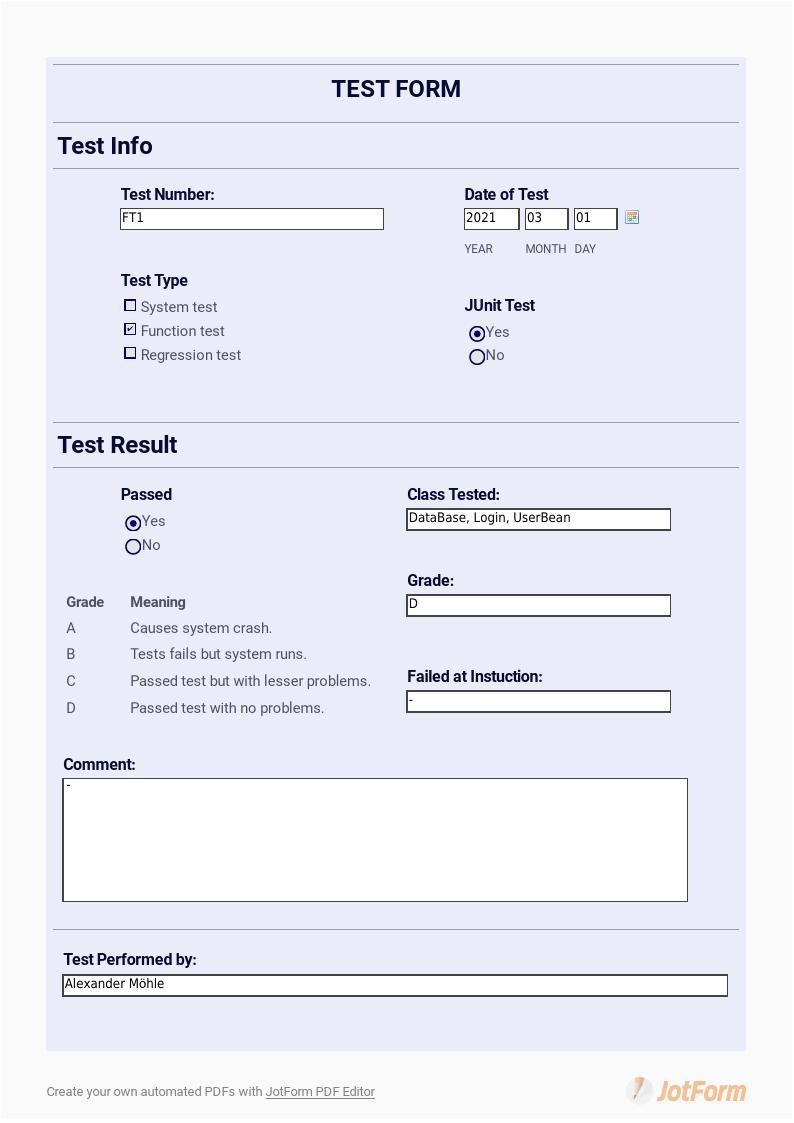
\includegraphics[trim={1cm 3cm 1cm 1.5cm}, clip,width=13cm]{images/2021_03_01_Alexander_FT1_001}
     \renewcommand\figurename{Figure}
     \caption{Test form for FT1}
     \label{fig:my_label}
 \end{figure}
 
 \begin{figure}
     \centering
     \includegraphics[trim={1cm 3cm 1cm 1.5cm},clip,width=13cm]
     {images/2021-03-01_Alexander_FT2_001}
     \renewcommand\figurename{Figure}
     \caption{Test form for FT2}
     \label{fig:my_label}
 \end{figure}
 
  \begin{figure}
     \centering
      \includegraphics[trim={1cm 3cm 1cm 1.5cm}, clip,width=13cm]
      {images/2021-03-03_Malte_FT3-1}
     \renewcommand\figurename{Figure}
     \caption{Test form for FT3}
     \label{fig:my_label}
 \end{figure}
 
 \begin{figure}
     \centering
      \includegraphics[trim={1cm 3cm 1cm 1.5cm}, clip,width=13cm]   	{images/2021-03-03_Malte_FT4-1}
     \renewcommand\figurename{Figure}
     \caption{Test form for FT4}
     \label{fig:my_label}
 \end{figure}

\begin{figure}
     \centering
      \includegraphics[trim={1cm 3cm 1cm 1.5cm}, clip,width=13cm]{images/2021-03-03_Malte_FT5-1}
     \renewcommand\figurename{Figure}
     \caption{Test form for FT5}
     \label{fig:my_label}
 \end{figure}
 
 \begin{figure}
     \centering
     \includegraphics[trim={1cm 3cm 1cm 1.5cm}, clip,width=13cm]{images/2021-03-04_Alexander_FT6-1}
     \renewcommand\figurename{Figure}
     \caption{Test form for FT6}
     \label{fig:my_label}
 \end{figure}
 
 \begin{figure}
     \centering
      \includegraphics[trim={1cm 3cm 1cm 1.5cm}, clip,width=13cm]{images/2021-03-04_Alexander_FT7-1}
     \renewcommand\figurename{Figure}
     \caption{Test form for FT7}
     \label{fig:my_label}
 \end{figure}
 
 \begin{figure}
     \centering
     \includegraphics[trim={1cm 3cm 1cm 1.5cm}, clip,width=13cm]{images/2021-03-03_Lazar_FT8-1}
     \renewcommand\figurename{Figure}
     \caption{Test form for FT8}
     \label{fig:my_label}
 \end{figure}
 
 \begin{figure}
     \centering
      \includegraphics[trim={1cm 3cm 1cm 1.5cm}, clip,width=13cm]{images/2021-03-03_Lazar_FT9-1}
     \renewcommand\figurename{Figure}
     \caption{Test form for FT9}
     \label{fig:my_label}
 \end{figure}
 
 \begin{figure}
     \centering
      \includegraphics[trim={1cm 3cm 1cm 1.5cm}, clip,width=13cm]{images/2021-03-03_Malte_FT10-1}
     \renewcommand\figurename{Figure}
     \caption{Test form for FT10}
     \label{fig:my_label}
 \end{figure}
 
 \begin{figure}
     \centering
     \includegraphics[trim={1cm 3cm 1cm 1.5cm}, clip,width=13cm]{images/2021-03-03_Lazar_FT11-1}
     \renewcommand\figurename{Figure}
     \caption{Test form for FT11}
     \label{fig:my_label}
 \end{figure}
 
 \begin{figure}
     \centering
     \ \includegraphics[trim={1cm 3cm 1cm 1.5cm}, clip,width=13cm]{images/2021-03-03_Lazar_FT12-1}
     \renewcommand\figurename{Figure}
     \caption{Test form for FT12}
     \label{fig:my_label}
 \end{figure}
 
 \begin{figure}
     \centering
     \includegraphics[trim={1cm 3cm 1cm 1.5cm}, clip,width=13cm]{images/2021-03-02_Alexander_FT18_001}
     \renewcommand\figurename{Figure}
     \caption{Test form for FT18}
     \label{fig:my_label}
 \end{figure}
 
 \begin{figure}
     \centering
     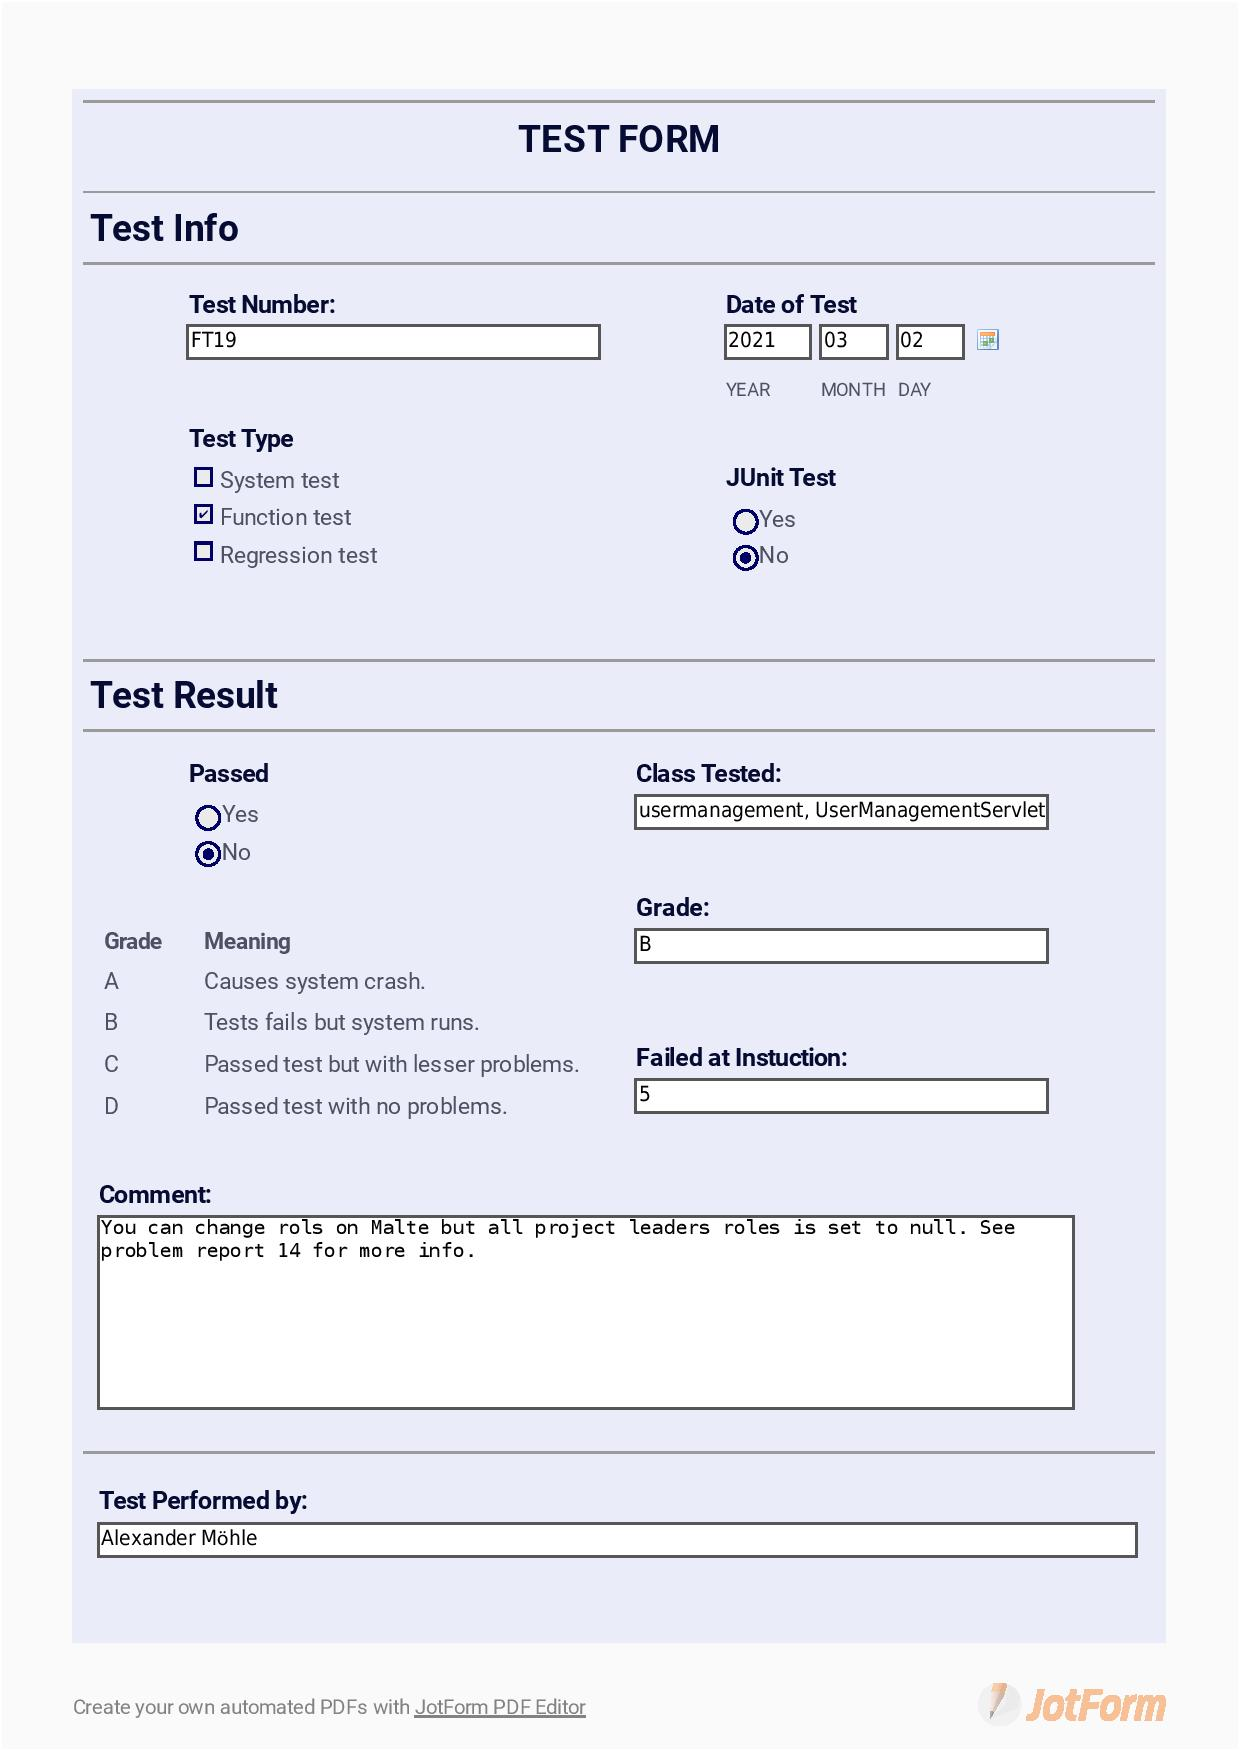
\includegraphics[trim={1cm 3cm 1cm 1.5cm}, clip,width=13cm]{images/2021-03-02_Alexander_FT19_001}
     \renewcommand\figurename{Figure}
     \caption{Test form for FT19}
     \label{fig:my_label}
 \end{figure}
 
 \begin{figure}
     \centering
     \includegraphics[trim={1cm 3cm 1cm 1.5cm}, clip,width=13cm]{images/2021-03-02_Alexander_FT20_001}
     \renewcommand\figurename{Figure}
     \caption{Test form for FT20}
     \label{fig:my_label}
 \end{figure}
 
 \begin{figure}
     \centering
      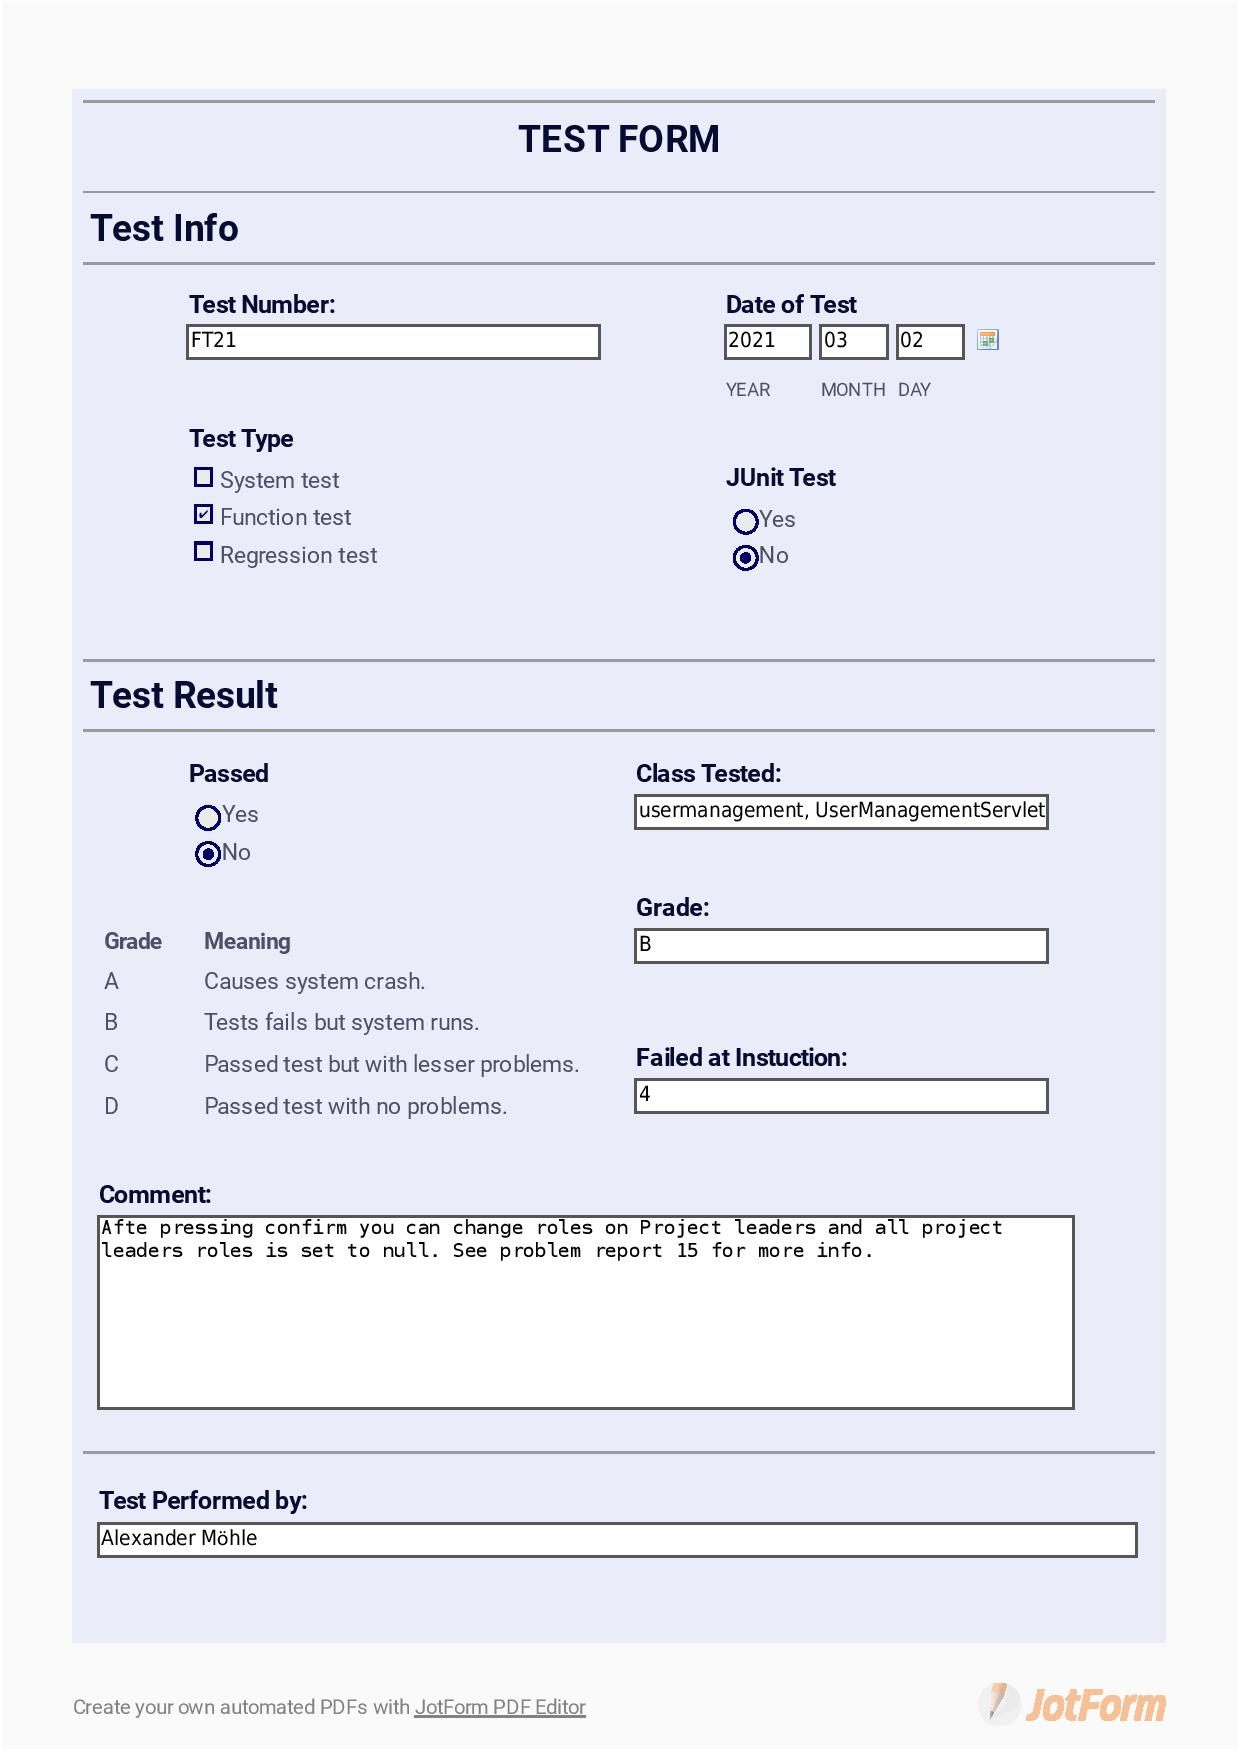
\includegraphics[trim={1cm 3cm 1cm 1.5cm}, clip,width=13cm]{images/2021-03-02_Alexander_FT21_001}
     \renewcommand\figurename{Figure}
     \caption{Test form for FT21}
     \label{fig:my_label}
 \end{figure}
 
 \begin{figure}
     \centering
      \includegraphics[trim={1cm 3cm 1cm 1.5cm}, clip,width=13cm]{images/2021-03-04_Alexander_FT24-1}
     \renewcommand\figurename{Figure}
     \caption{Test form for FT24}
     \label{fig:my_label}
 \end{figure}
 
 \begin{figure}
     \centering
      \includegraphics[trim={1cm 3cm 1cm 2cm}, clip,width=13cm]{images/2021-03-03_Anas_FT25-1}
     \renewcommand\figurename{Figure}
     \caption{Test form for FT25}
     \label{fig:my_label}
 \end{figure}
 
 \begin{figure}
     \centering
    \includegraphics[trim={1cm 3cm 1cm 2cm}, clip,width=13cm]{images/2021-03-03_Anas_FT26-1}
     \renewcommand\figurename{Figure}
     \caption{Test form for FT26}
     \label{fig:my_label}
 \end{figure}
 
 \begin{figure}
     \centering
     \includegraphics[trim={1cm 3cm 1cm 2cm}, clip,width=13cm]{images/2021-03-03_Anas_FT27-1}
     \renewcommand\figurename{Figure}
     \caption{Test form for FT27}
     \label{fig:my_label}
 \end{figure}
 
 \begin{figure}
     \centering
      \includegraphics[trim={1cm 3cm 1cm 1.5cm}, clip,width=13cm]{images/2021-03-02_Alexander_FT29_001}
     \renewcommand\figurename{Figure}
     \caption{Test form for FT29}
     \label{fig:my_label}
 \end{figure}
 
 \begin{figure}
     \centering
     \includegraphics[trim={1cm 3cm 1cm 1.5cm}, clip,width=13cm]{images/2021-03-02_Alexander_FT30_001}
     \renewcommand\figurename{Figure}
     \caption{Test form for FT30}
     \label{fig:my_label}
 \end{figure}
 
 \begin{figure}
     \centering
     \includegraphics[trim={1cm 3cm 1cm 1.5cm}, clip,width=13cm]{images/2021-03-03_Alexander_FT31_001}
     \renewcommand\figurename{Figure}
     \caption{Test form for FT31}
     \label{fig:my_label}
 \end{figure}


\newpage
\begin{flushleft}
{\large \textbf{B. Regression Test Result}}
\end{flushleft}


 \begin{figure}
     \centering
      \includegraphics[trim={1cm 3cm 1cm 1.5cm}, clip,width=13cm]{images/2021-03-03_Alexander_RT1(FT1, FT18)-1.jpg}
     \renewcommand\figurename{Figure}
     \caption{Regression test form for RT1 (FT1,FT18)}
     \label{fig:my_label}
 \end{figure}
 
  \begin{figure}
     \centering
      \includegraphics[trim={1cm 3cm 1cm 1.5cm}, clip,width=13cm]{images/2021-03-03_Alexander_RT1(FT1, FT19)-1.jpg}
     \renewcommand\figurename{Figure}
     \caption{Regression test form for RT1 (FT1,FT19)}
     \label{fig:my_label}
 \end{figure}
 
  \begin{figure}
     \centering
      \includegraphics[trim={1cm 3cm 1cm 1.5cm}, clip,width=13cm]{images/2021-03-03_Alexander_RT1(FT1, FT20)-1.jpg}
     \renewcommand\figurename{Figure}
     \caption{Regression test form for RT1 (FT1,FT20)}
     \label{fig:my_label}
 \end{figure}
 
  \begin{figure}
     \centering
      \includegraphics[trim={1cm 3cm 1cm 1.5cm}, clip,width=13cm]{images/2021-03-03_Alexander_RT1(FT1, FT21)-1.jpg}
     \renewcommand\figurename{Figure}
     \caption{Regression test form for RT1 (FT1,FT21)}
     \label{fig:my_label}
 \end{figure}
 

\newpage
\begin{flushleft}
{\large \textbf{C. System Test Result}}
\end{flushleft}


\begin{figure}
     \centering
     \includegraphics[trim={0cm 3.5cm 0cm 0cm}, clip,width=13cm]
     {images/2021-03-04_Alexander_ST1-1}
     \renewcommand\figurename{Figure}
     \label{fig:my_label}
 \end{figure}
 
 \begin{figure}
     \centering
     \includegraphics[trim={0cm 15cm 0cm 0cm}, clip,width=13cm]{images/2021-03-04_Alexander_ST1-2}
     \renewcommand\figurename{Figure}
     \caption{System test form for ST1 First Wave}
     \label{fig:my_label}
 \end{figure}


\begin{figure}
     \centering
     \includegraphics[trim={0cm 3.5cm 0cm 0cm}, clip,width=13cm]	{images/2021-03-04_Malte_ST2-1}
     \renewcommand\figurename{Figure}
     \label{fig:my_label}
 \end{figure}
 
 \begin{figure}
     \centering
      \includegraphics[trim={0cm 15cm 0cm 0cm}, clip,width=13cm]{images/2021-03-04_Malte_ST2-2}
     \renewcommand\figurename{Figure}
     \caption{System test form for ST2 First Wave}
     \label{fig:my_label}
 \end{figure}
 

\begin{figure}
     \centering
    \includegraphics[trim={0cm 3.5cm 0cm 0cm}, clip,width=13cm]{images/2021-03-04_Anas_ST3-1}
     \renewcommand\figurename{Figure}
     \label{fig:my_label}
 \end{figure}
 
 \begin{figure}
     \centering
     \includegraphics[trim={0cm 15cm 0cm 0cm}, clip,width=13cm]{images/2021-03-04_Anas_ST3-2}
     \renewcommand\figurename{Figure}
     \caption{System test form for ST3 First Wave}
     \label{fig:my_label}
 \end{figure}
 
 \begin{figure}
     \centering
     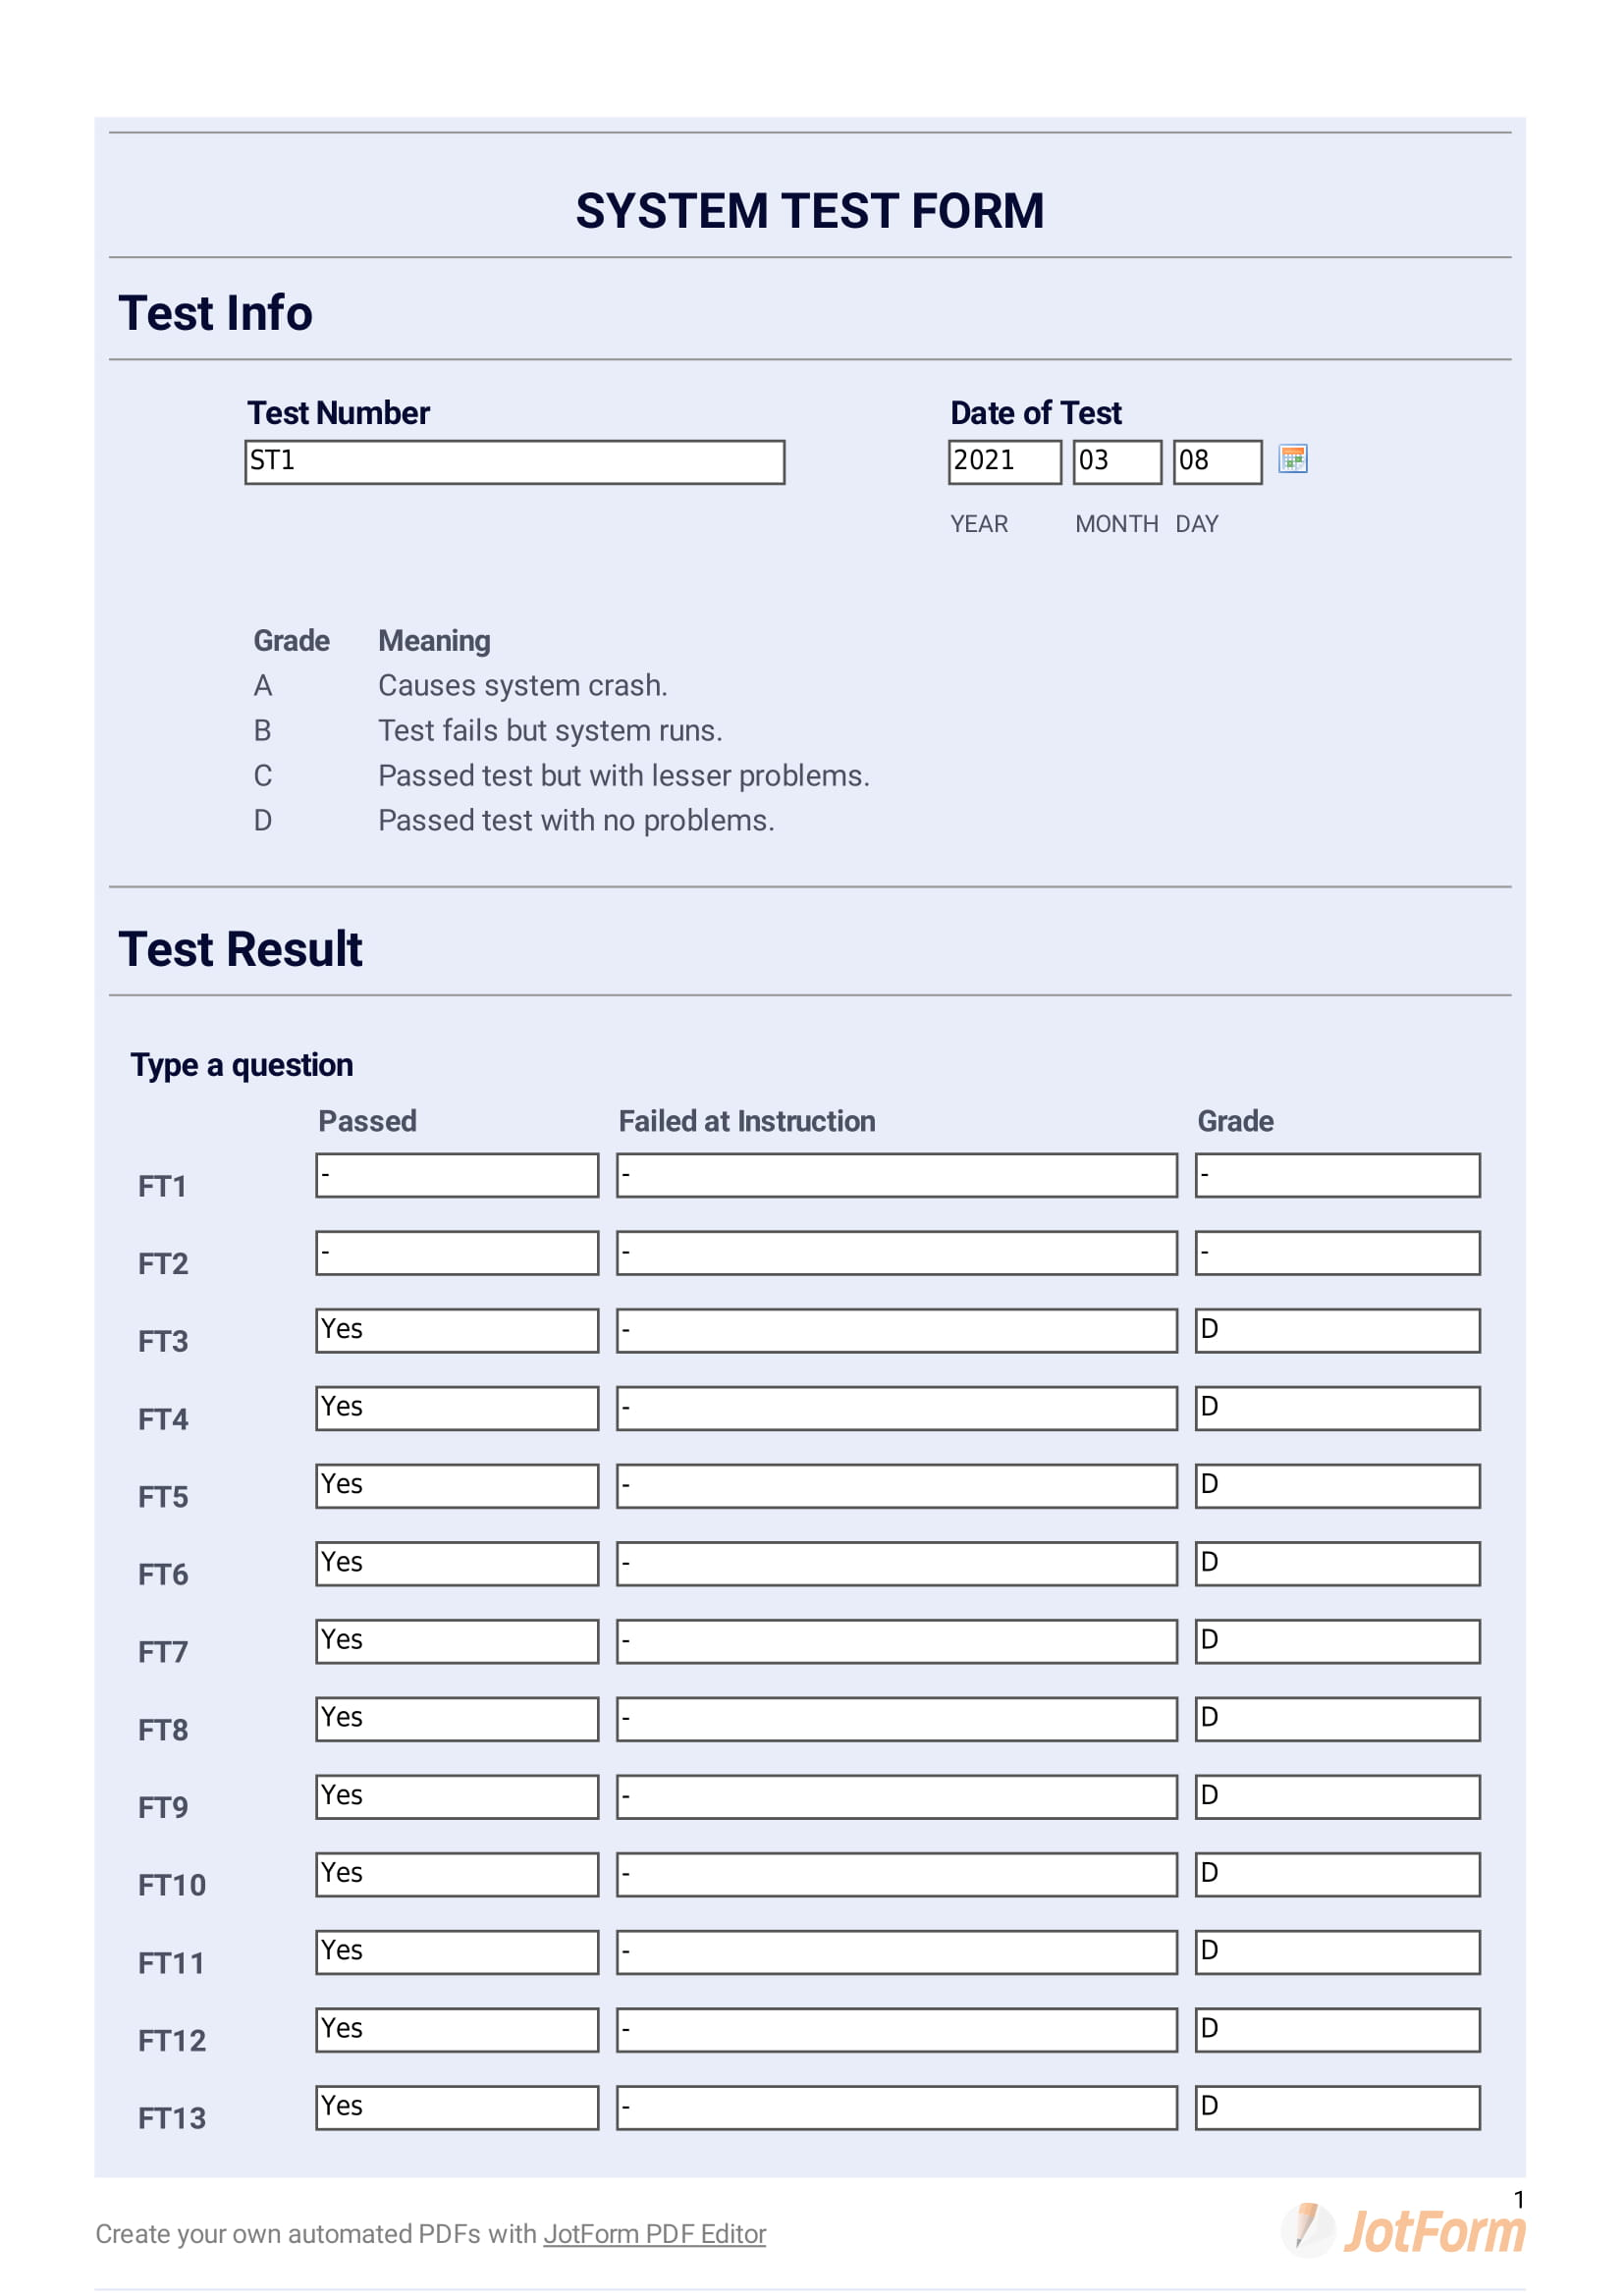
\includegraphics[trim={0cm 3.5cm 0cm 0cm}, clip,width=13cm]{images/2021-03-08_Alexander_ST1-1}
     \renewcommand\figurename{Figure}
     \label{fig:my_label}
 \end{figure}
 
 \begin{figure}
     \centering
     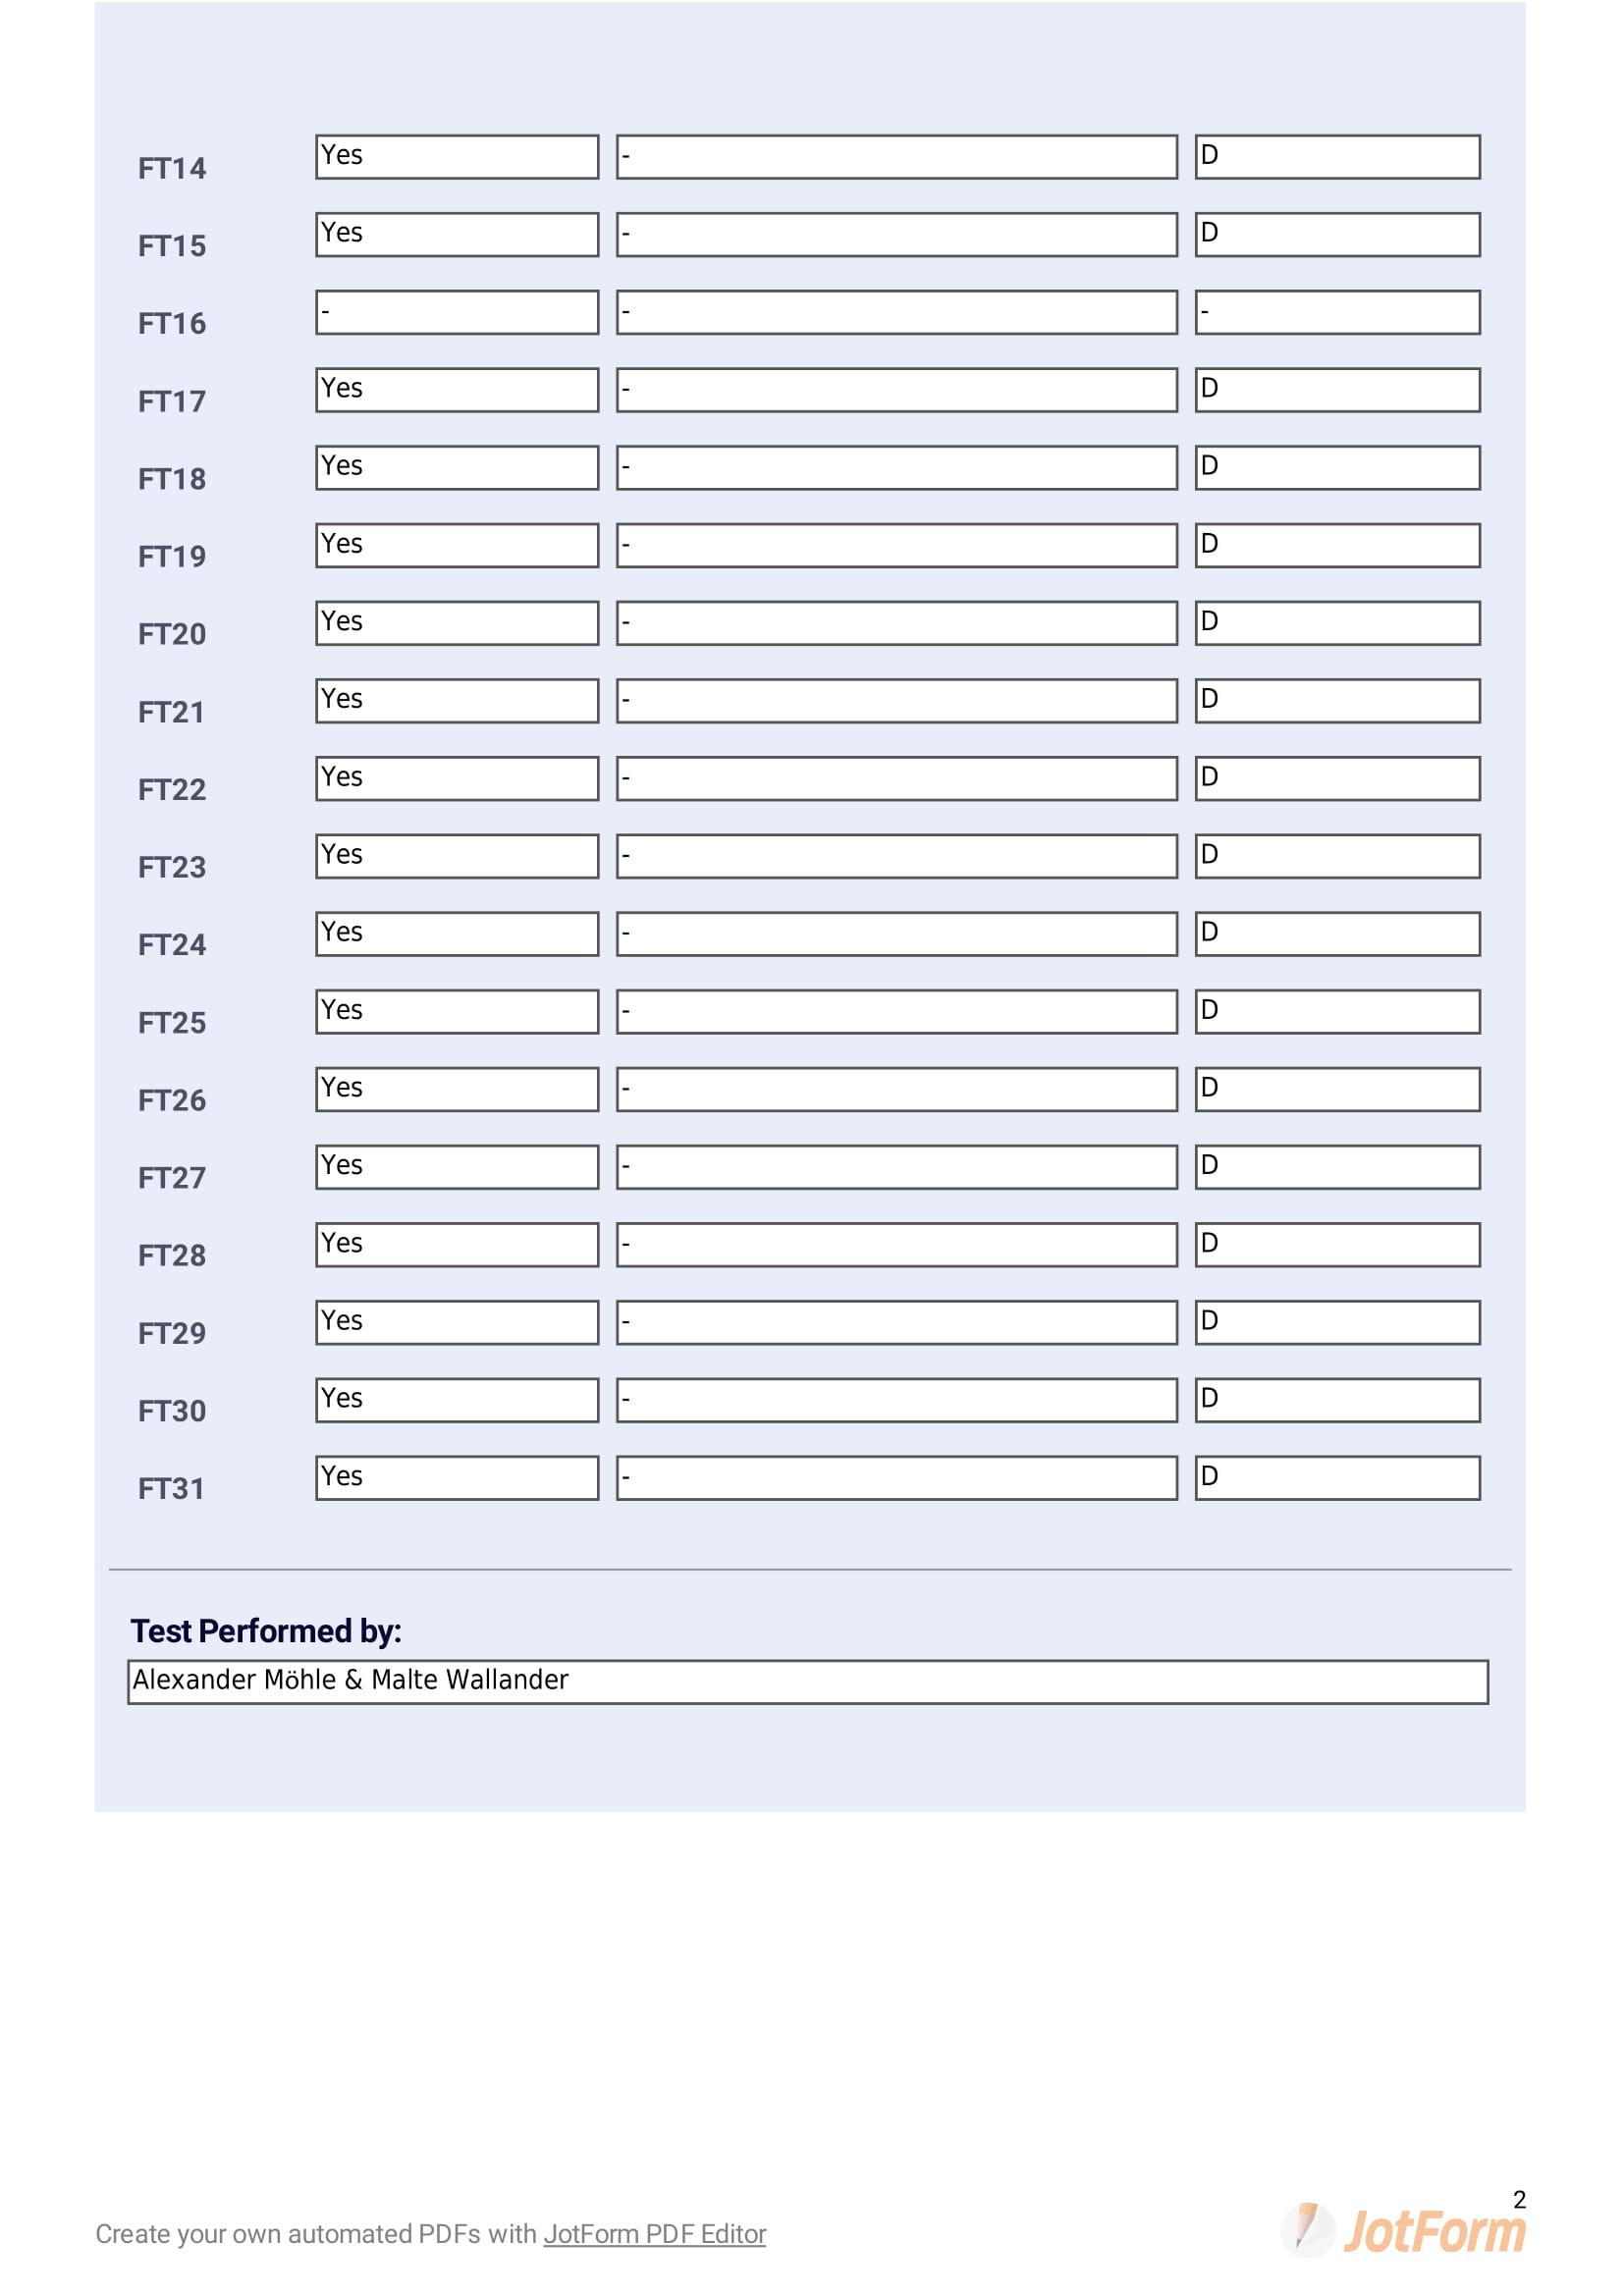
\includegraphics[trim={0cm 15cm 0cm 0cm}, clip,width=13cm]{images/2021-03-08_Alexander_ST1-2}
     \renewcommand\figurename{Figure}
     \caption{System test form for ST1 Second Wave}
     \label{fig:my_label}
 \end{figure}
 
 
 \begin{figure}
     \centering
    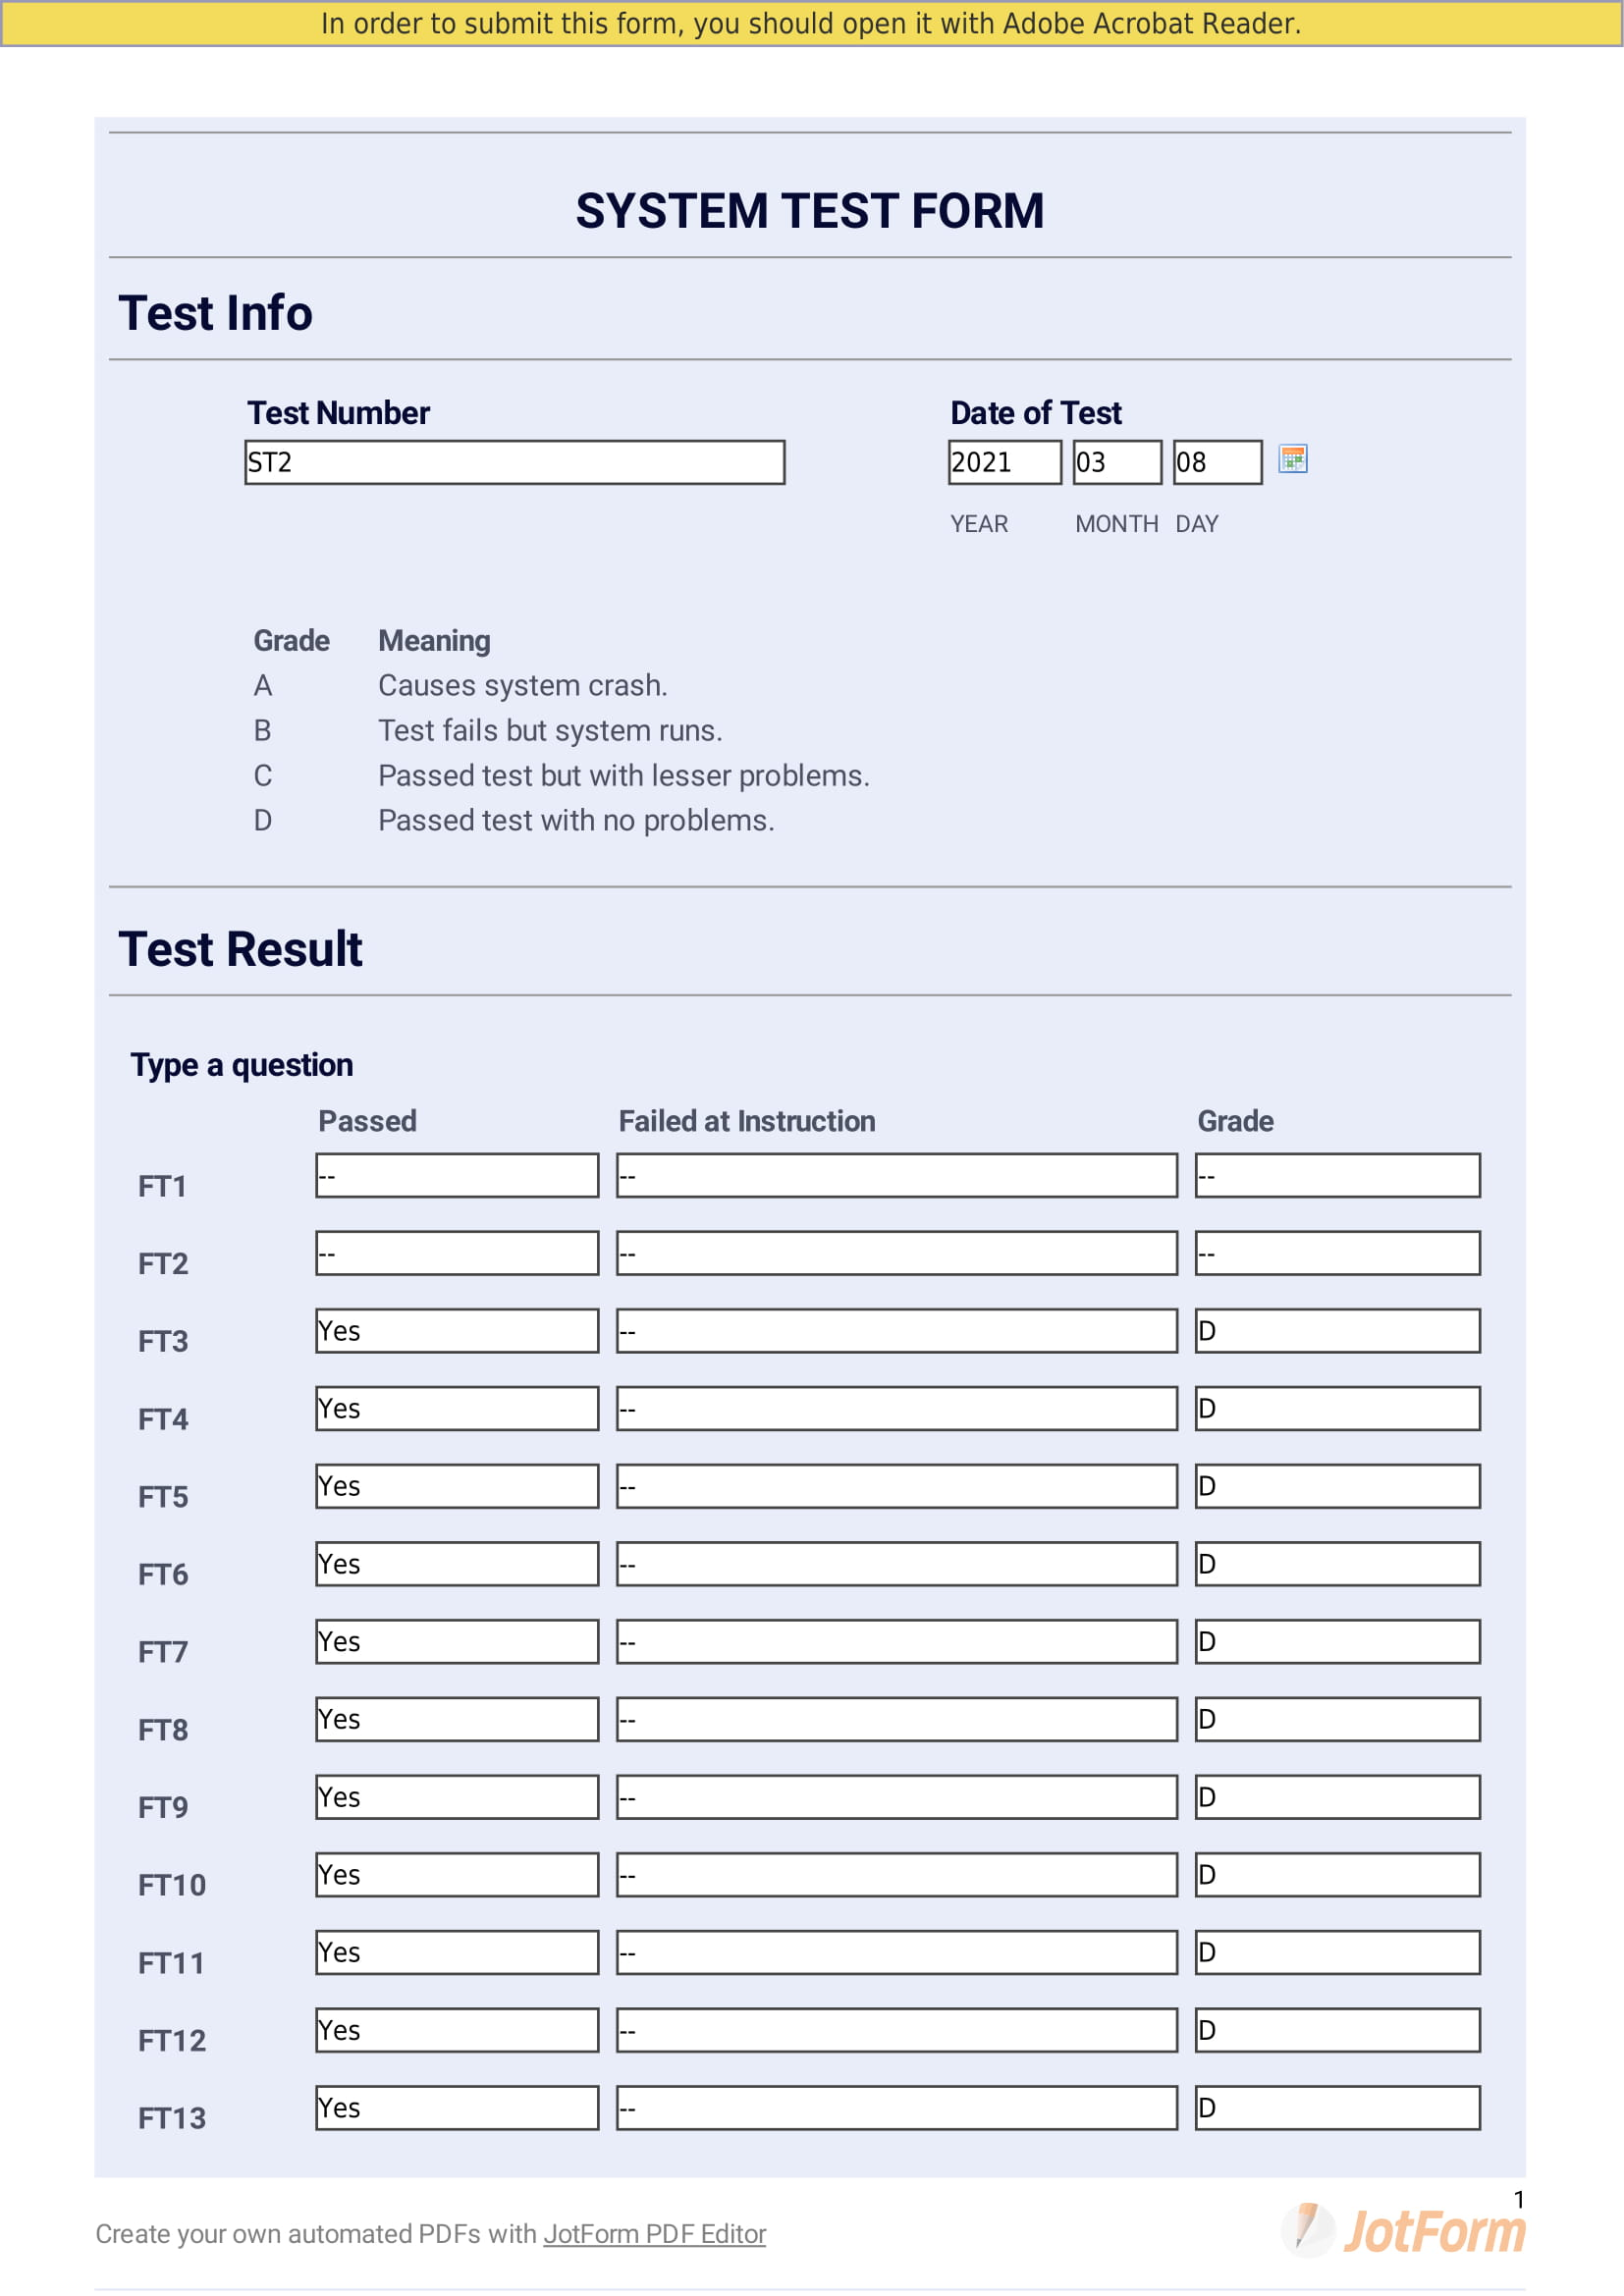
\includegraphics[trim={0cm 3.5cm 0cm 2cm}, clip,width=13cm]{images/2021-03-08_Malte_ST2-1}
     \renewcommand\figurename{Figure}
     \label{fig:my_label}
 \end{figure}
 
 \begin{figure}
     \centering
     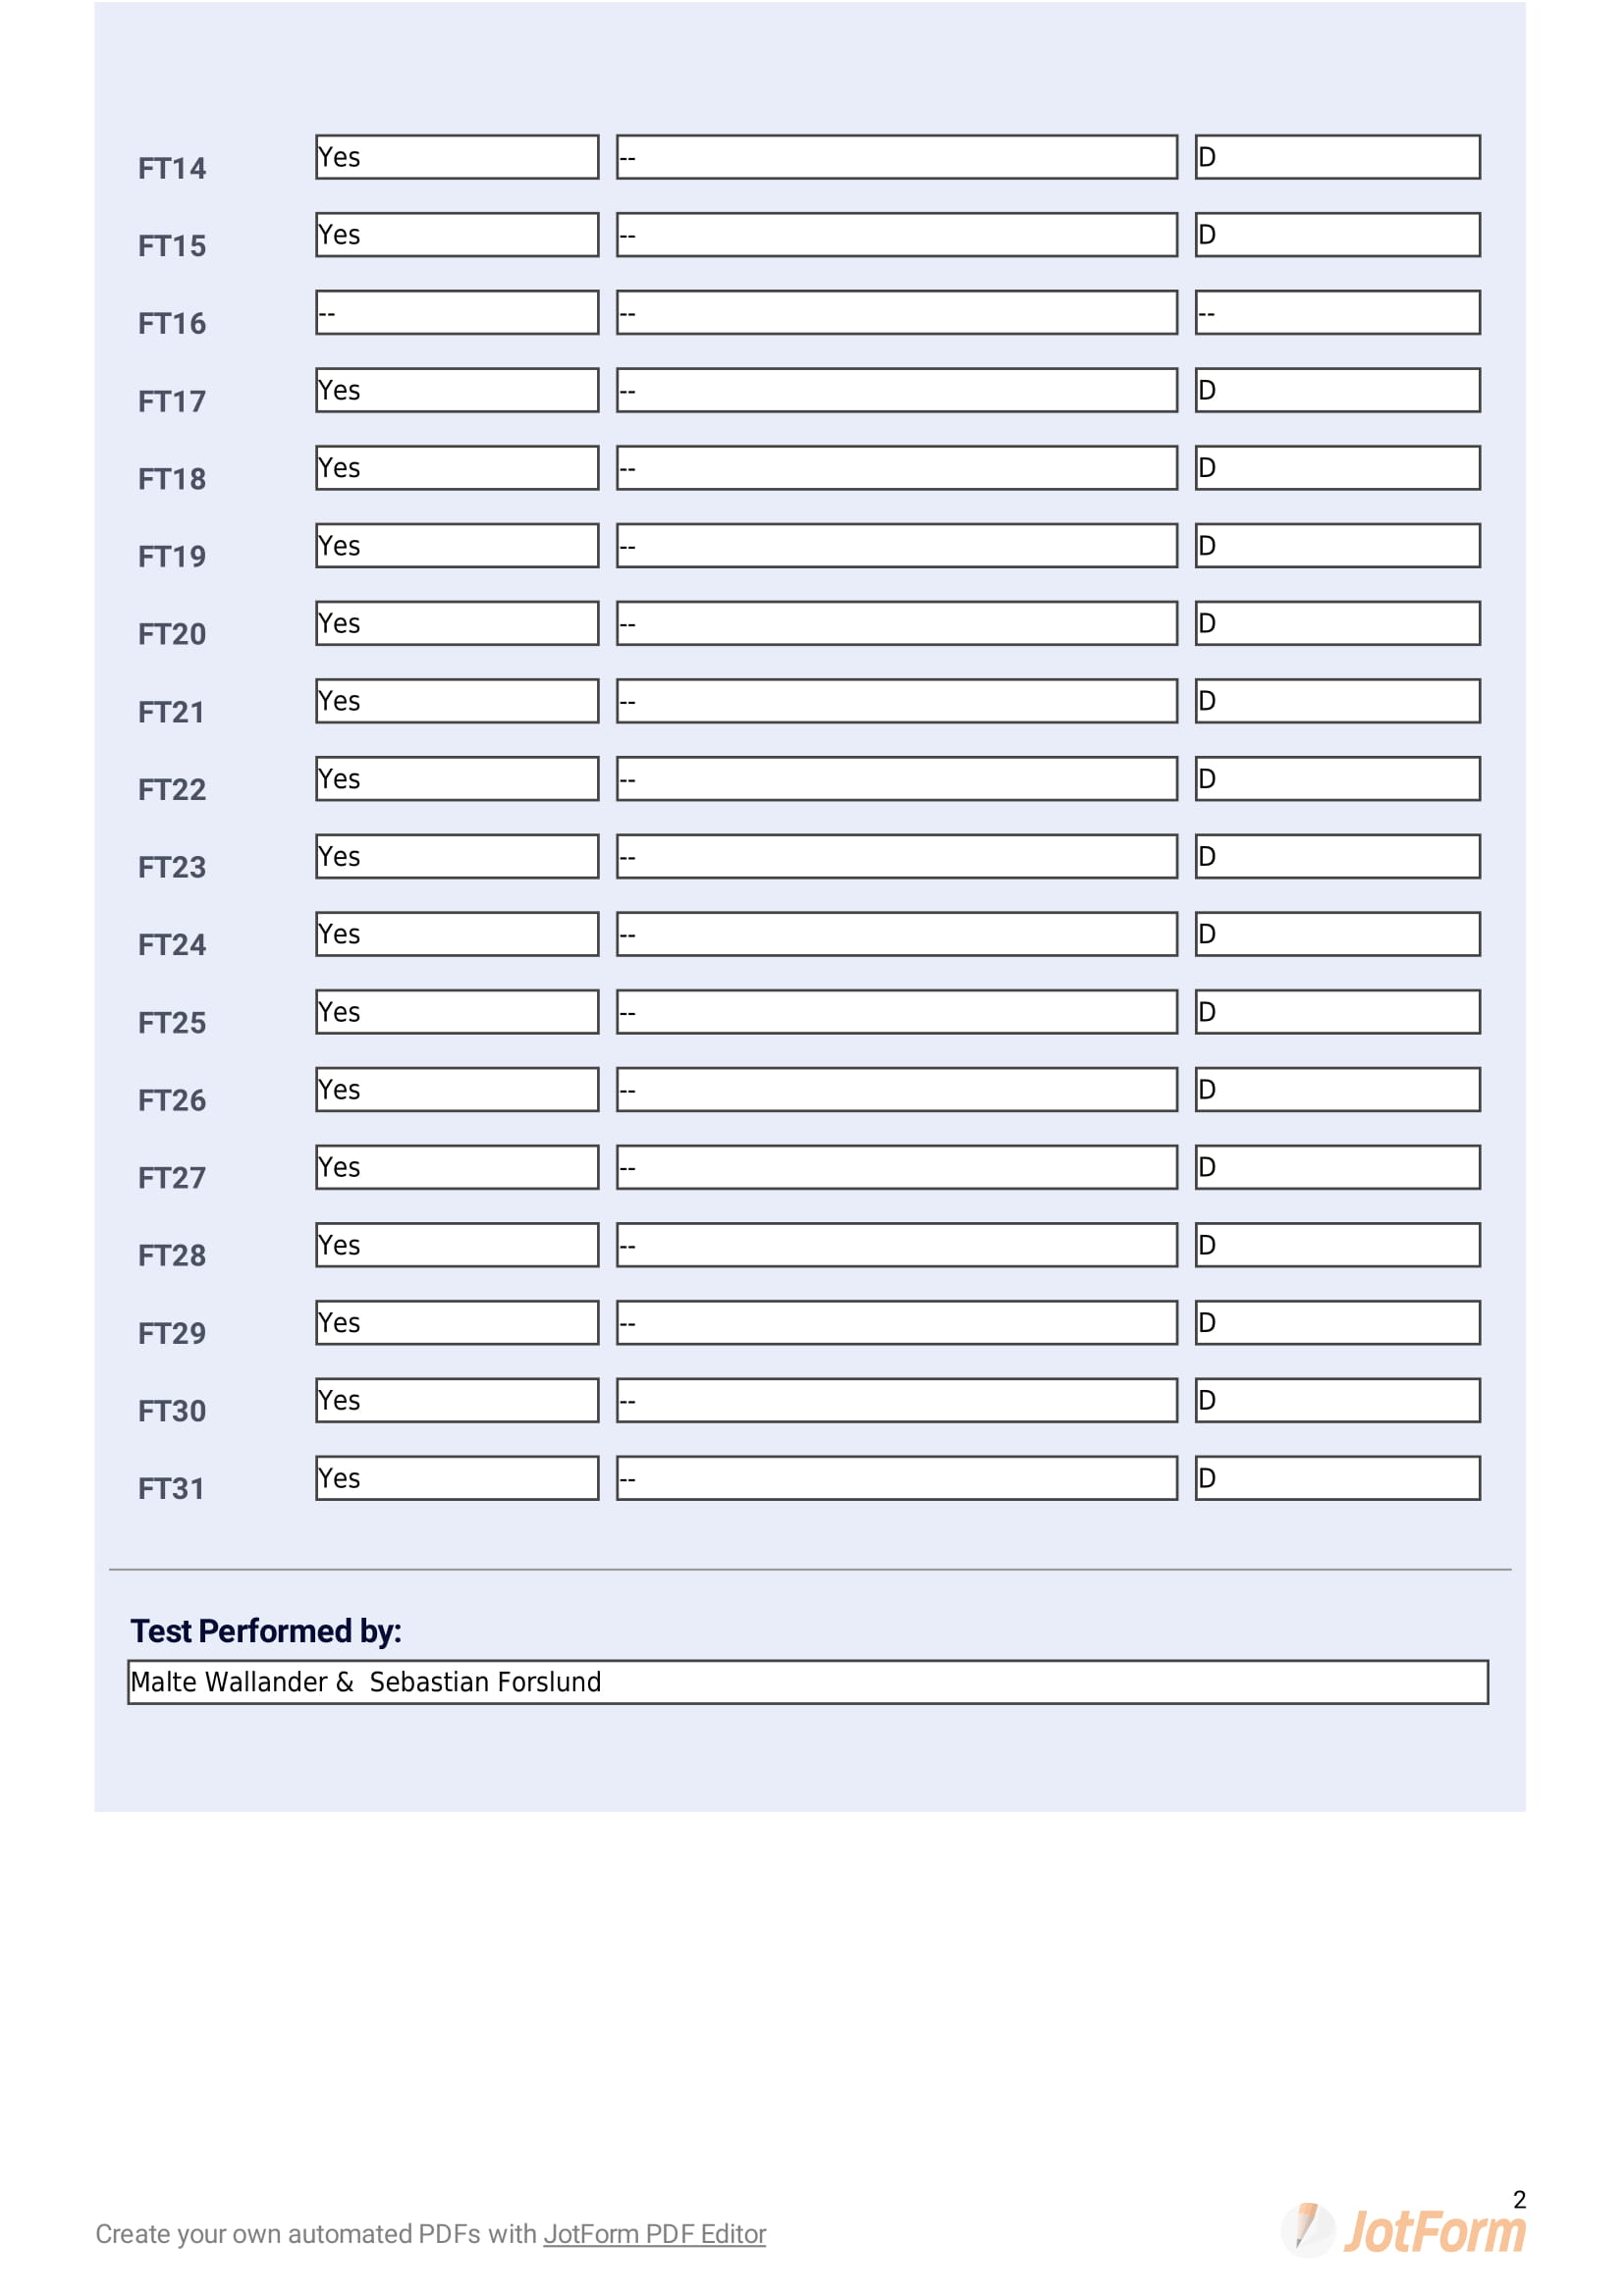
\includegraphics[trim={0cm 15cm 0cm 0cm}, clip,width=13cm]{images/2021-03-08_Malte_ST2-2}
     \renewcommand\figurename{Figure}
     \caption{System test form for ST2 Second Wave}
     \label{fig:my_label}
 \end{figure}


 \begin{figure}
     \centering
    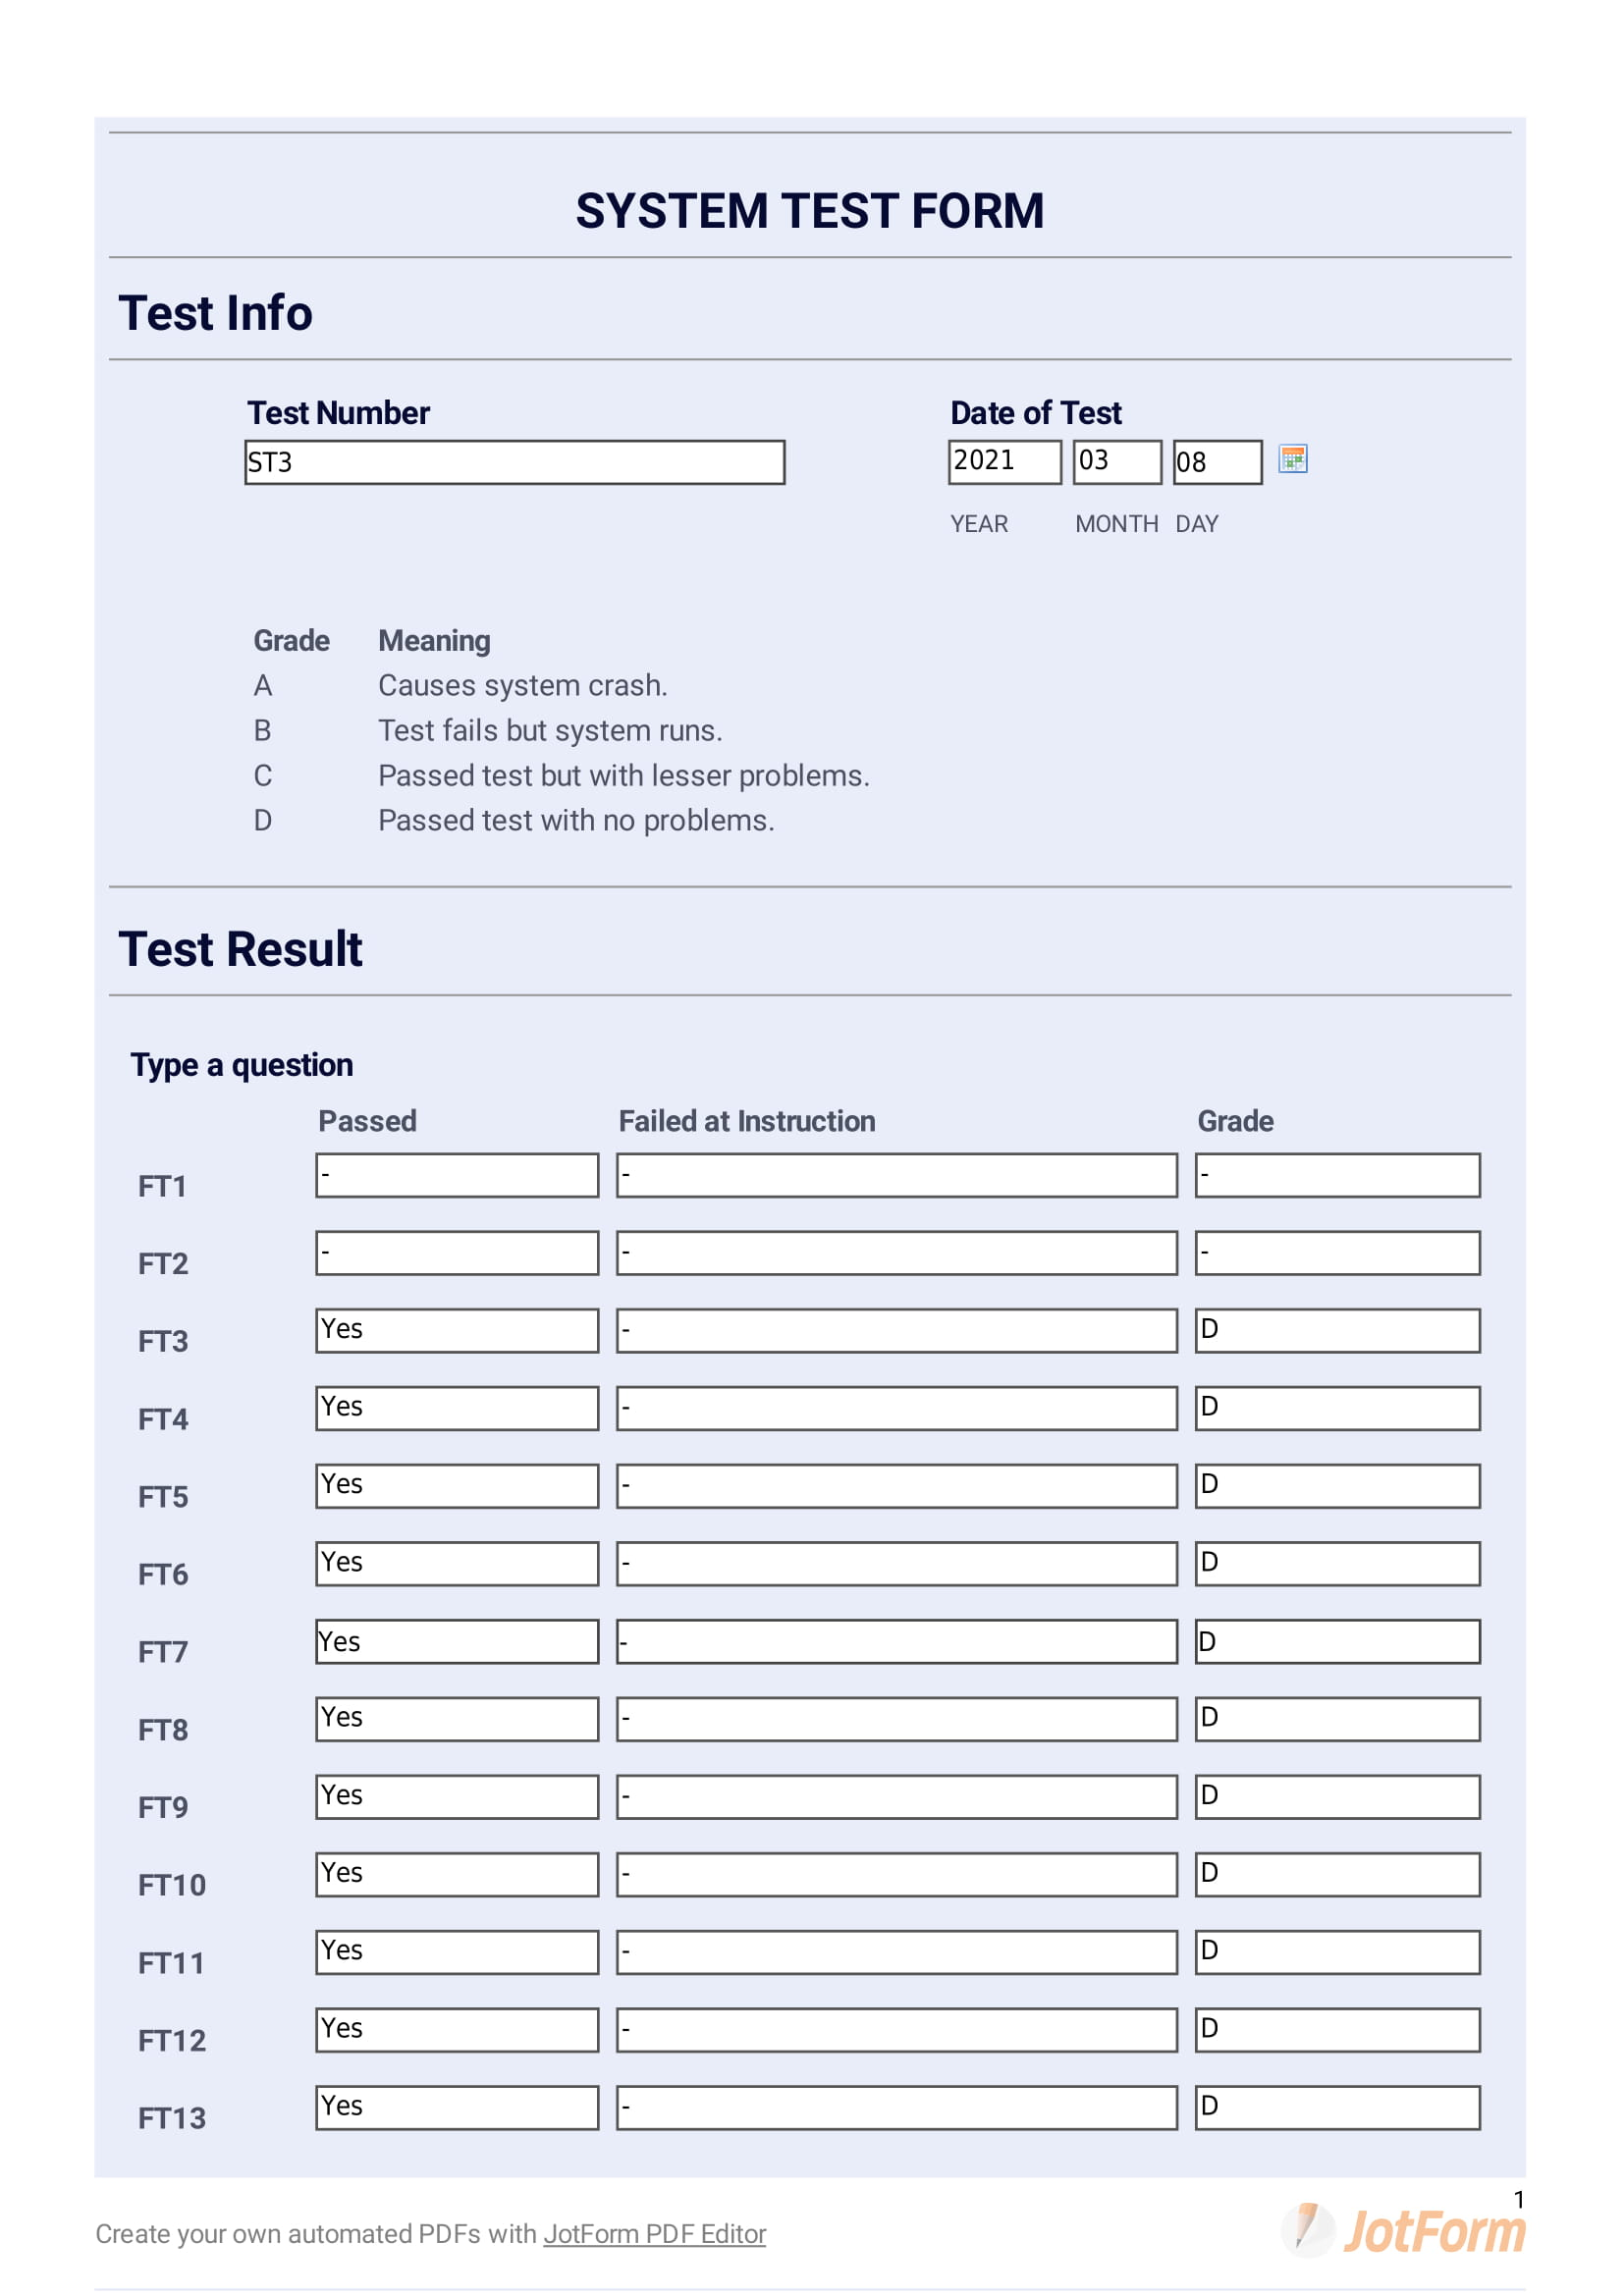
\includegraphics[trim={0cm 3.5cm 0cm 0cm}, clip,width=13cm]{images/2021-03-08_Anas_ST3-1}
     \renewcommand\figurename{Figure}
     \label{fig:my_label}
 \end{figure}
 
 \begin{figure}
     \centering
      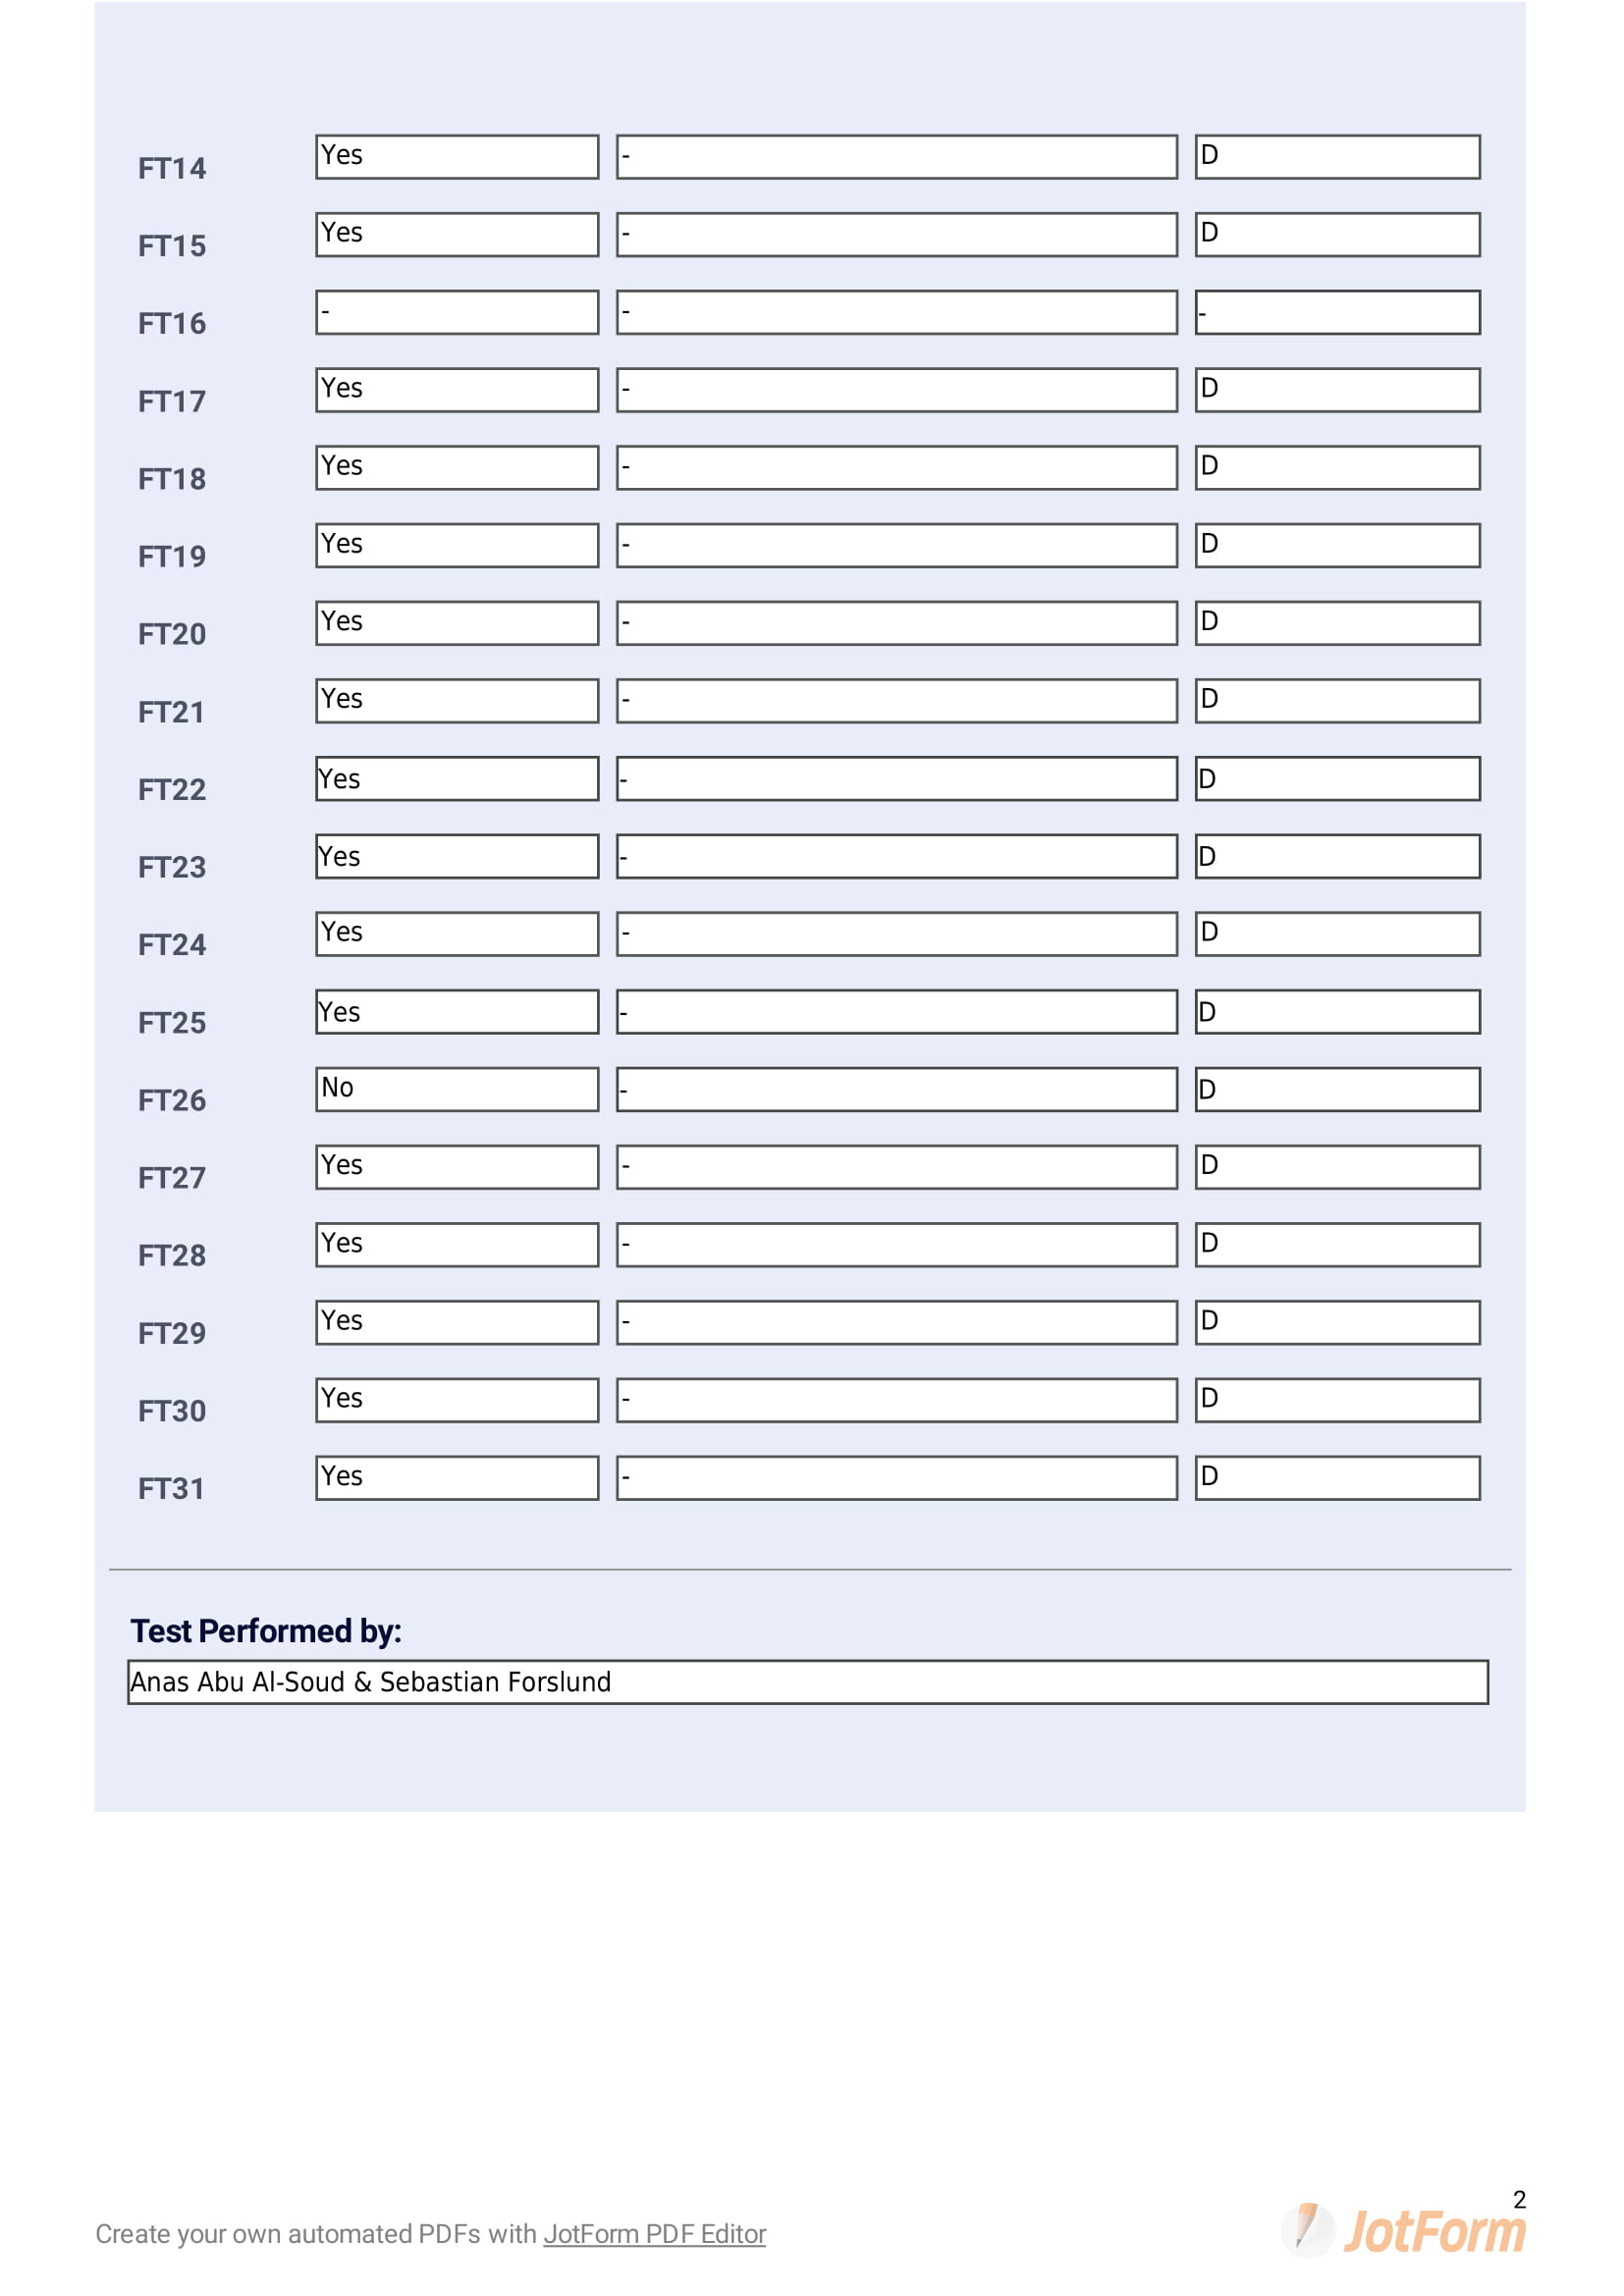
\includegraphics[trim={0cm 15cm 0cm 0cm}, clip,width=13cm]
      {images/2021-03-08_Anas_ST3-2}
     \renewcommand\figurename{Figure}
     \caption{System test form for ST3 Second Wave}
     \label{fig:my_label}
 \end{figure}

\newpage
\begin{flushleft}
{\large \textbf{D. Test Result in Google Sheet}}
\end{flushleft}



 \begin{figure}
     \centering
     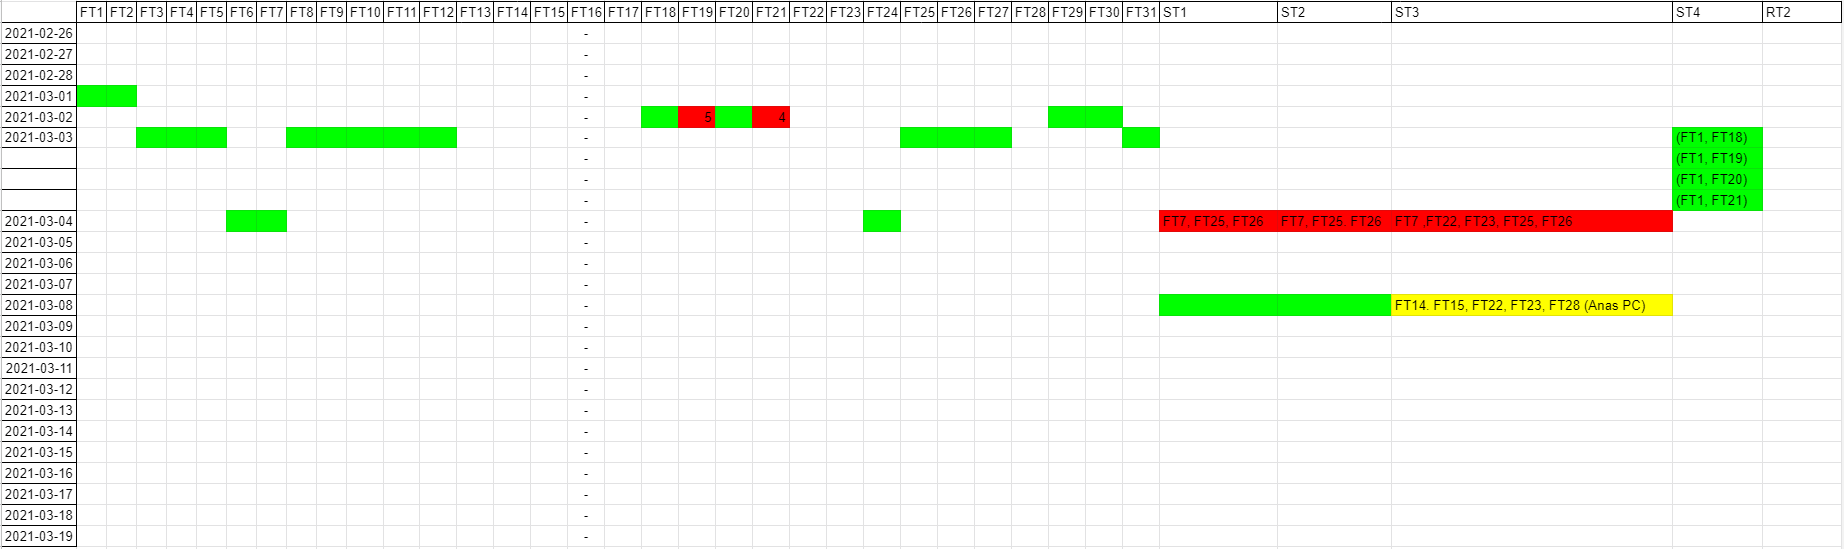
\includegraphics[scale = 0.5, angle = 270]{images/puspSheet}
     \renewcommand\figurename{Figure}
     \caption{Test Result in Google Sheet}
     \label{fig:my_label}
 \end{figure}


\newpage
\begin{flushleft}
{\large \textbf{E. Review Protocols}}
\end{flushleft}


\begin{figure}
     \centering
     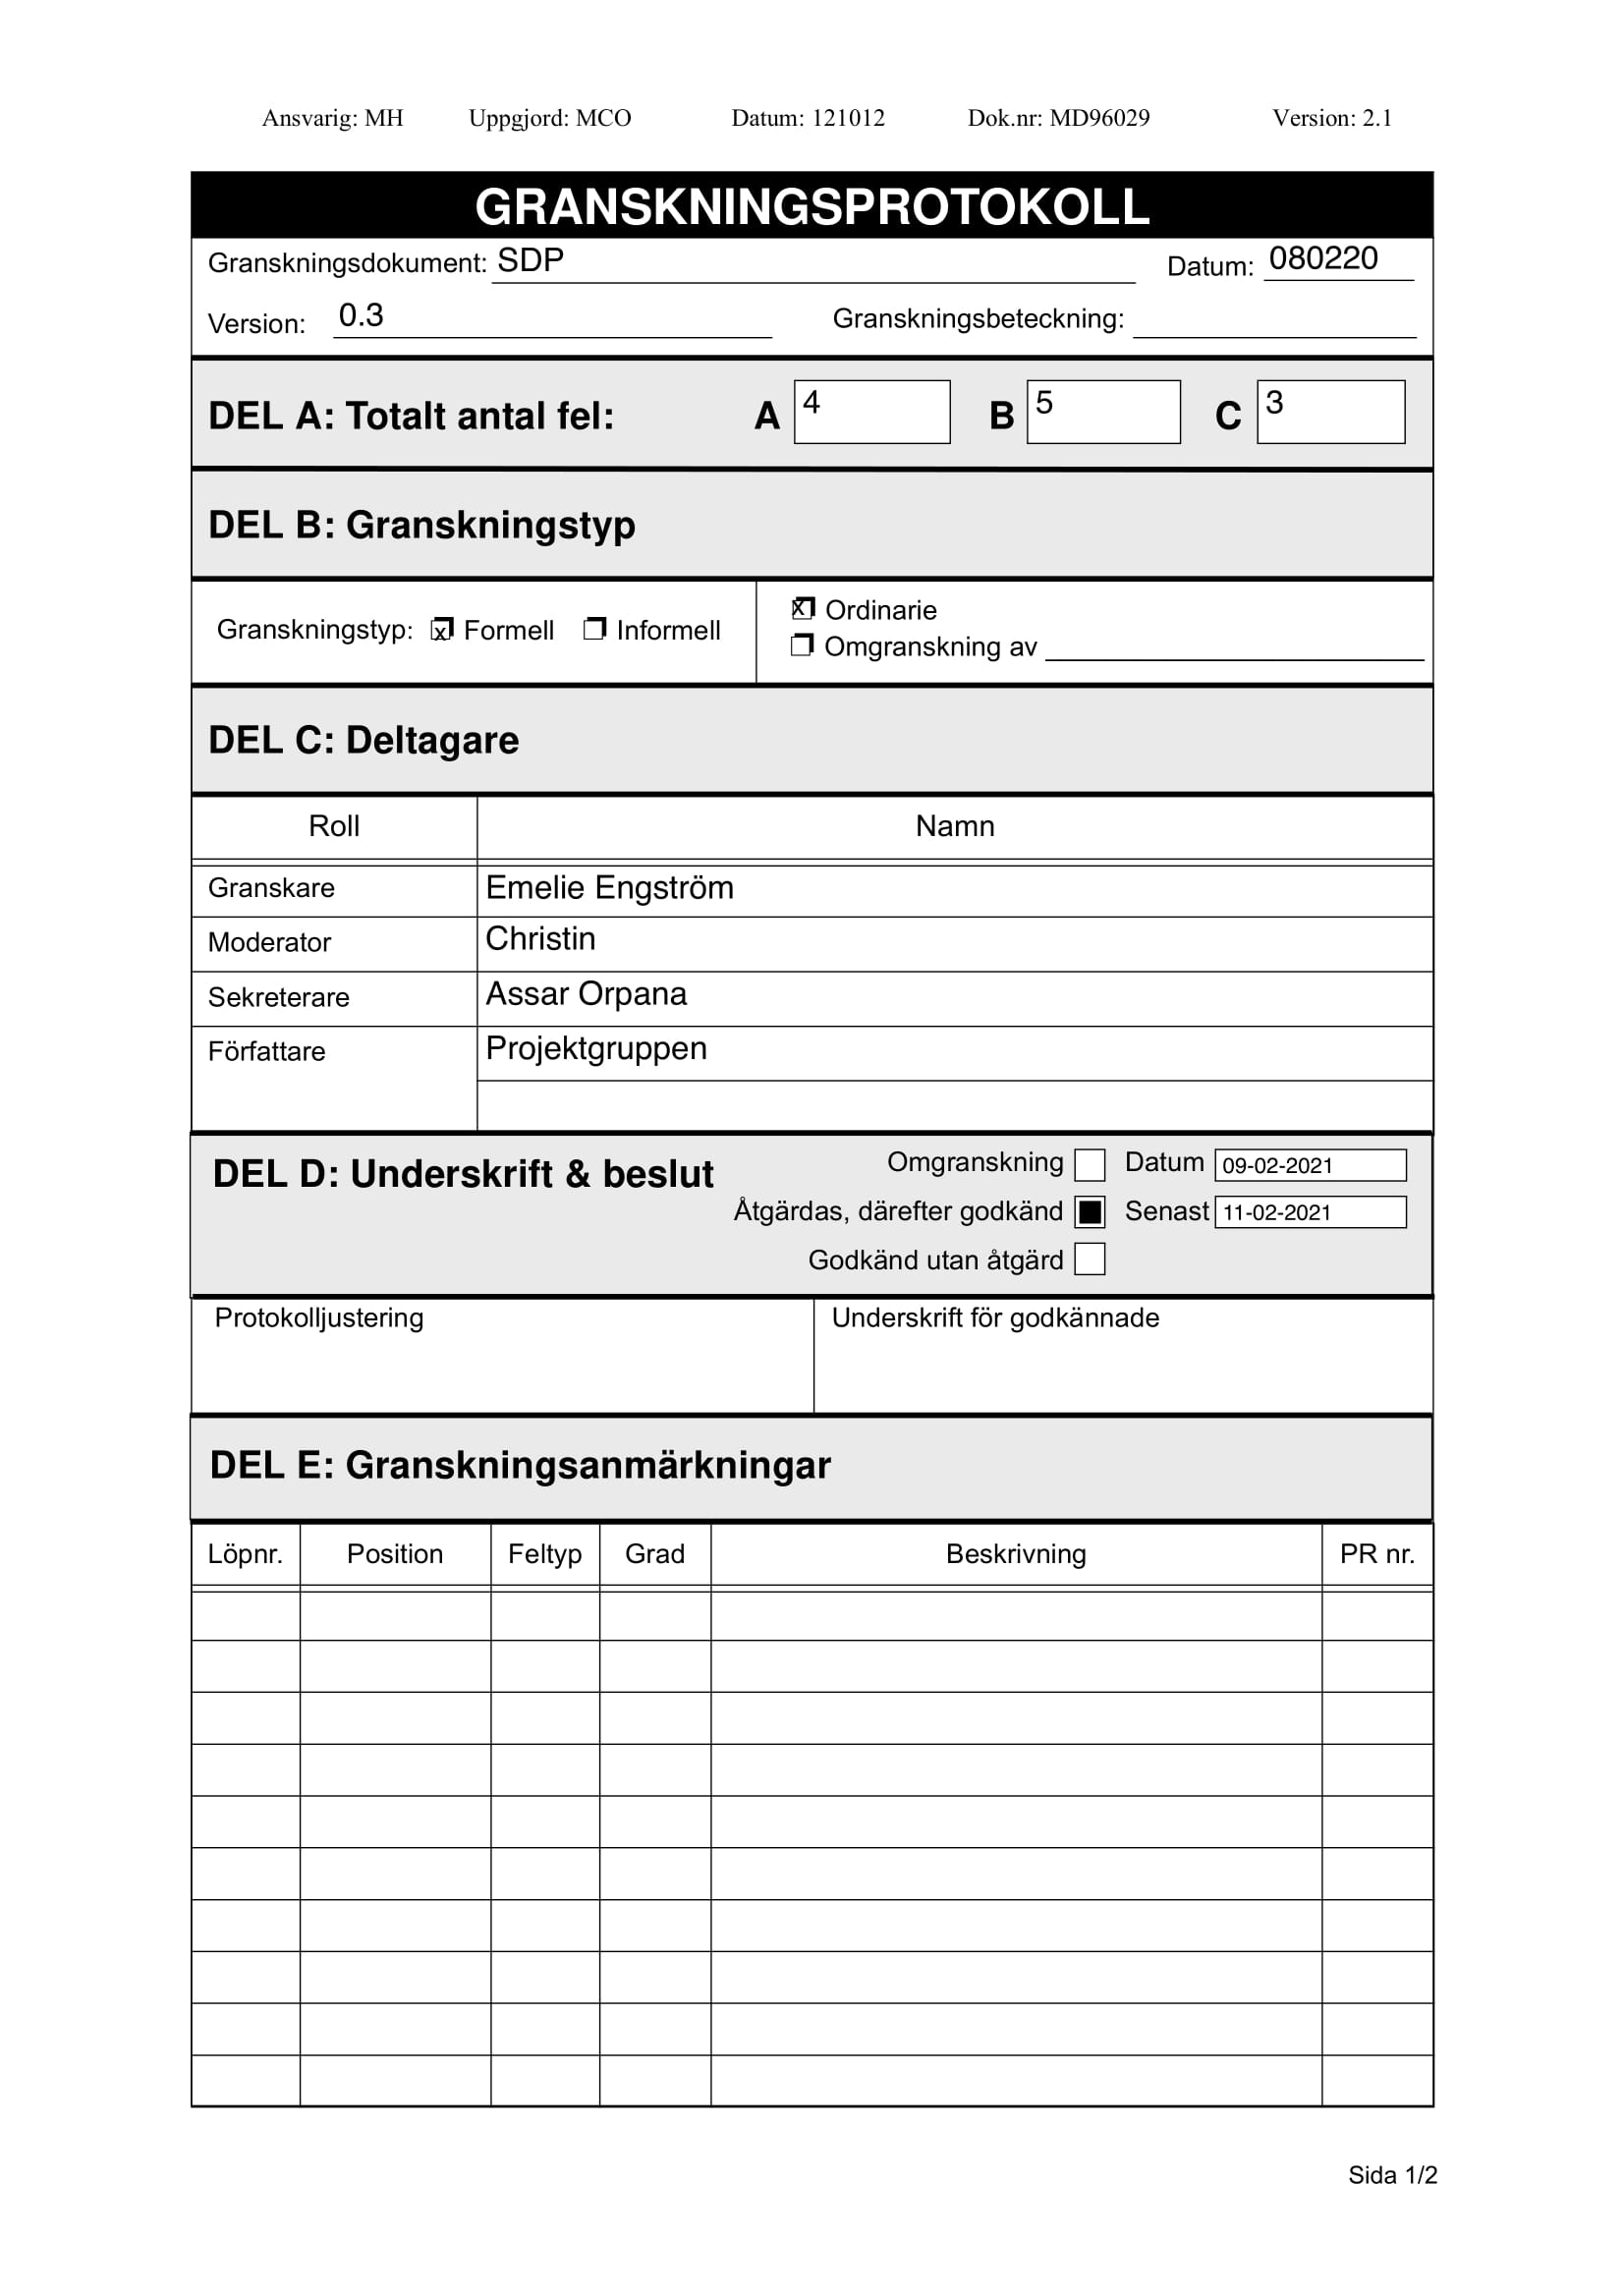
\includegraphics[width=13cm]{images/SDP - Granskningsprotokoll-1}
     \renewcommand\figurename{Figure}
      \caption{Review Protocol for SDP}
     \label{fig:my_label}
 \end{figure}
  
 
\begin{figure}
     \centering
     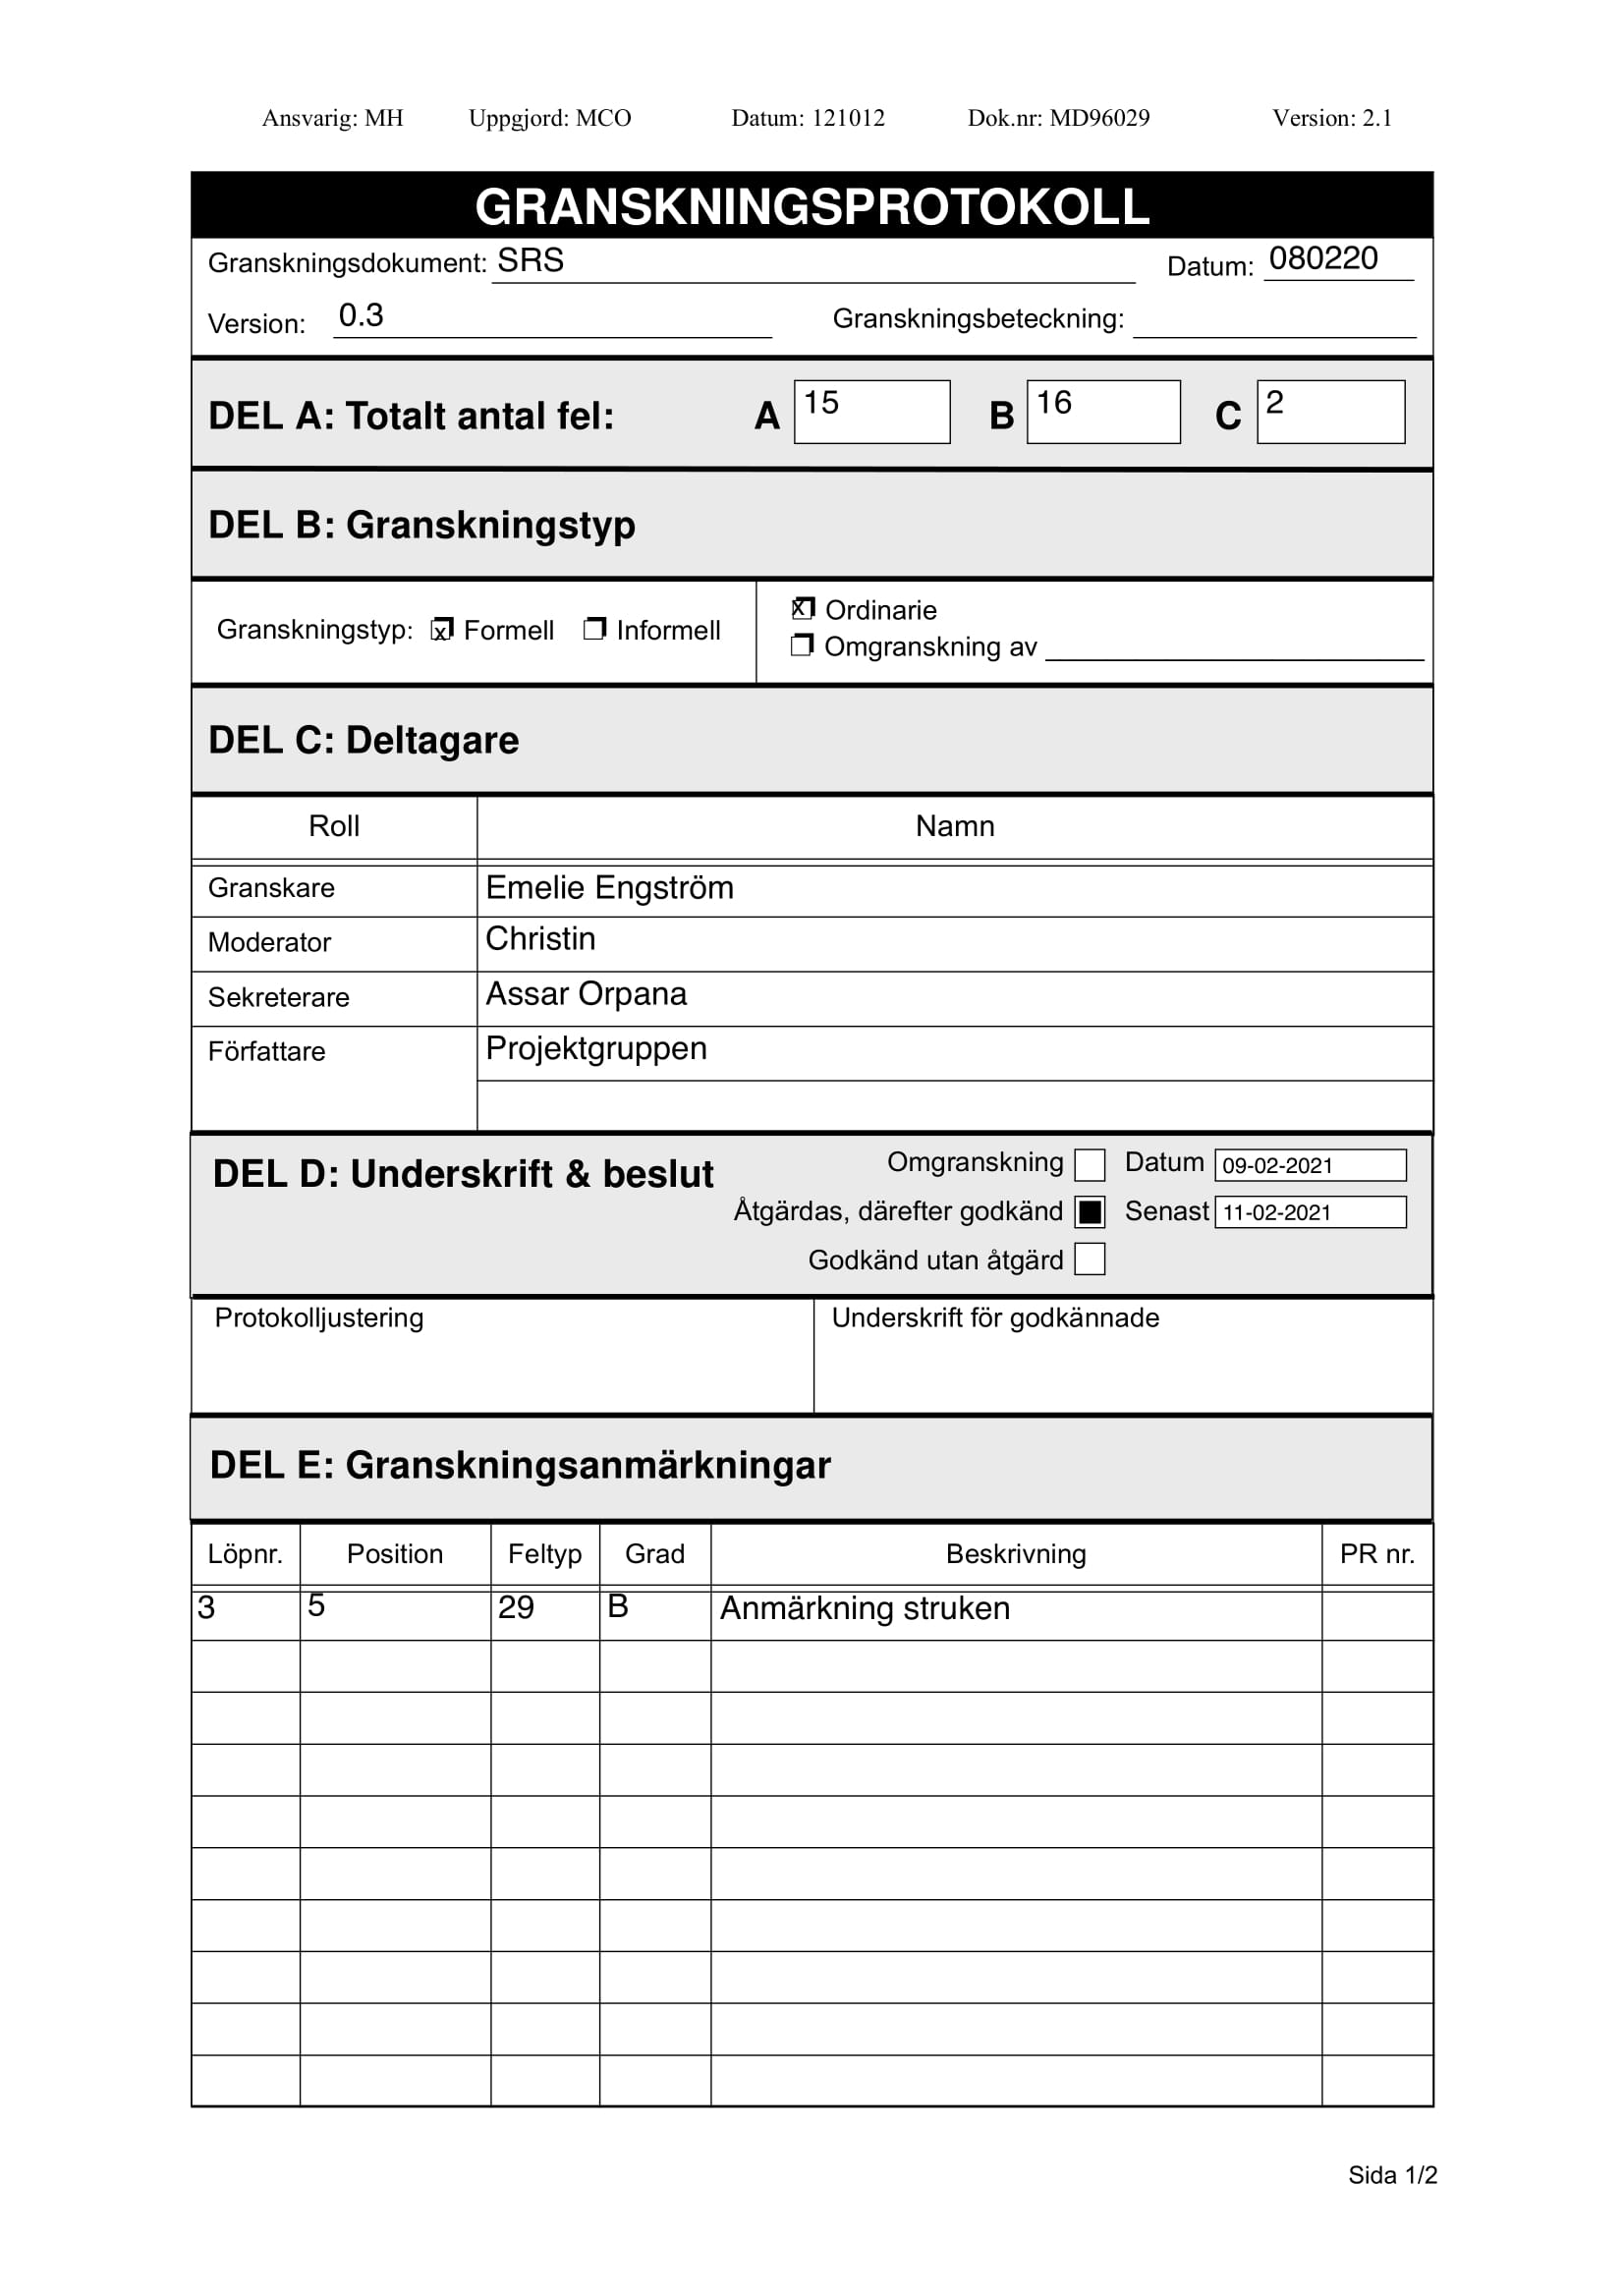
\includegraphics[width=13cm]{images/SRS - Granskningsprotokoll-1}
     \renewcommand\figurename{Figure}
      \caption{Review Protocol for SRS}
     \label{fig:my_label}
 \end{figure}
 

 
 \begin{figure}
     \centering
     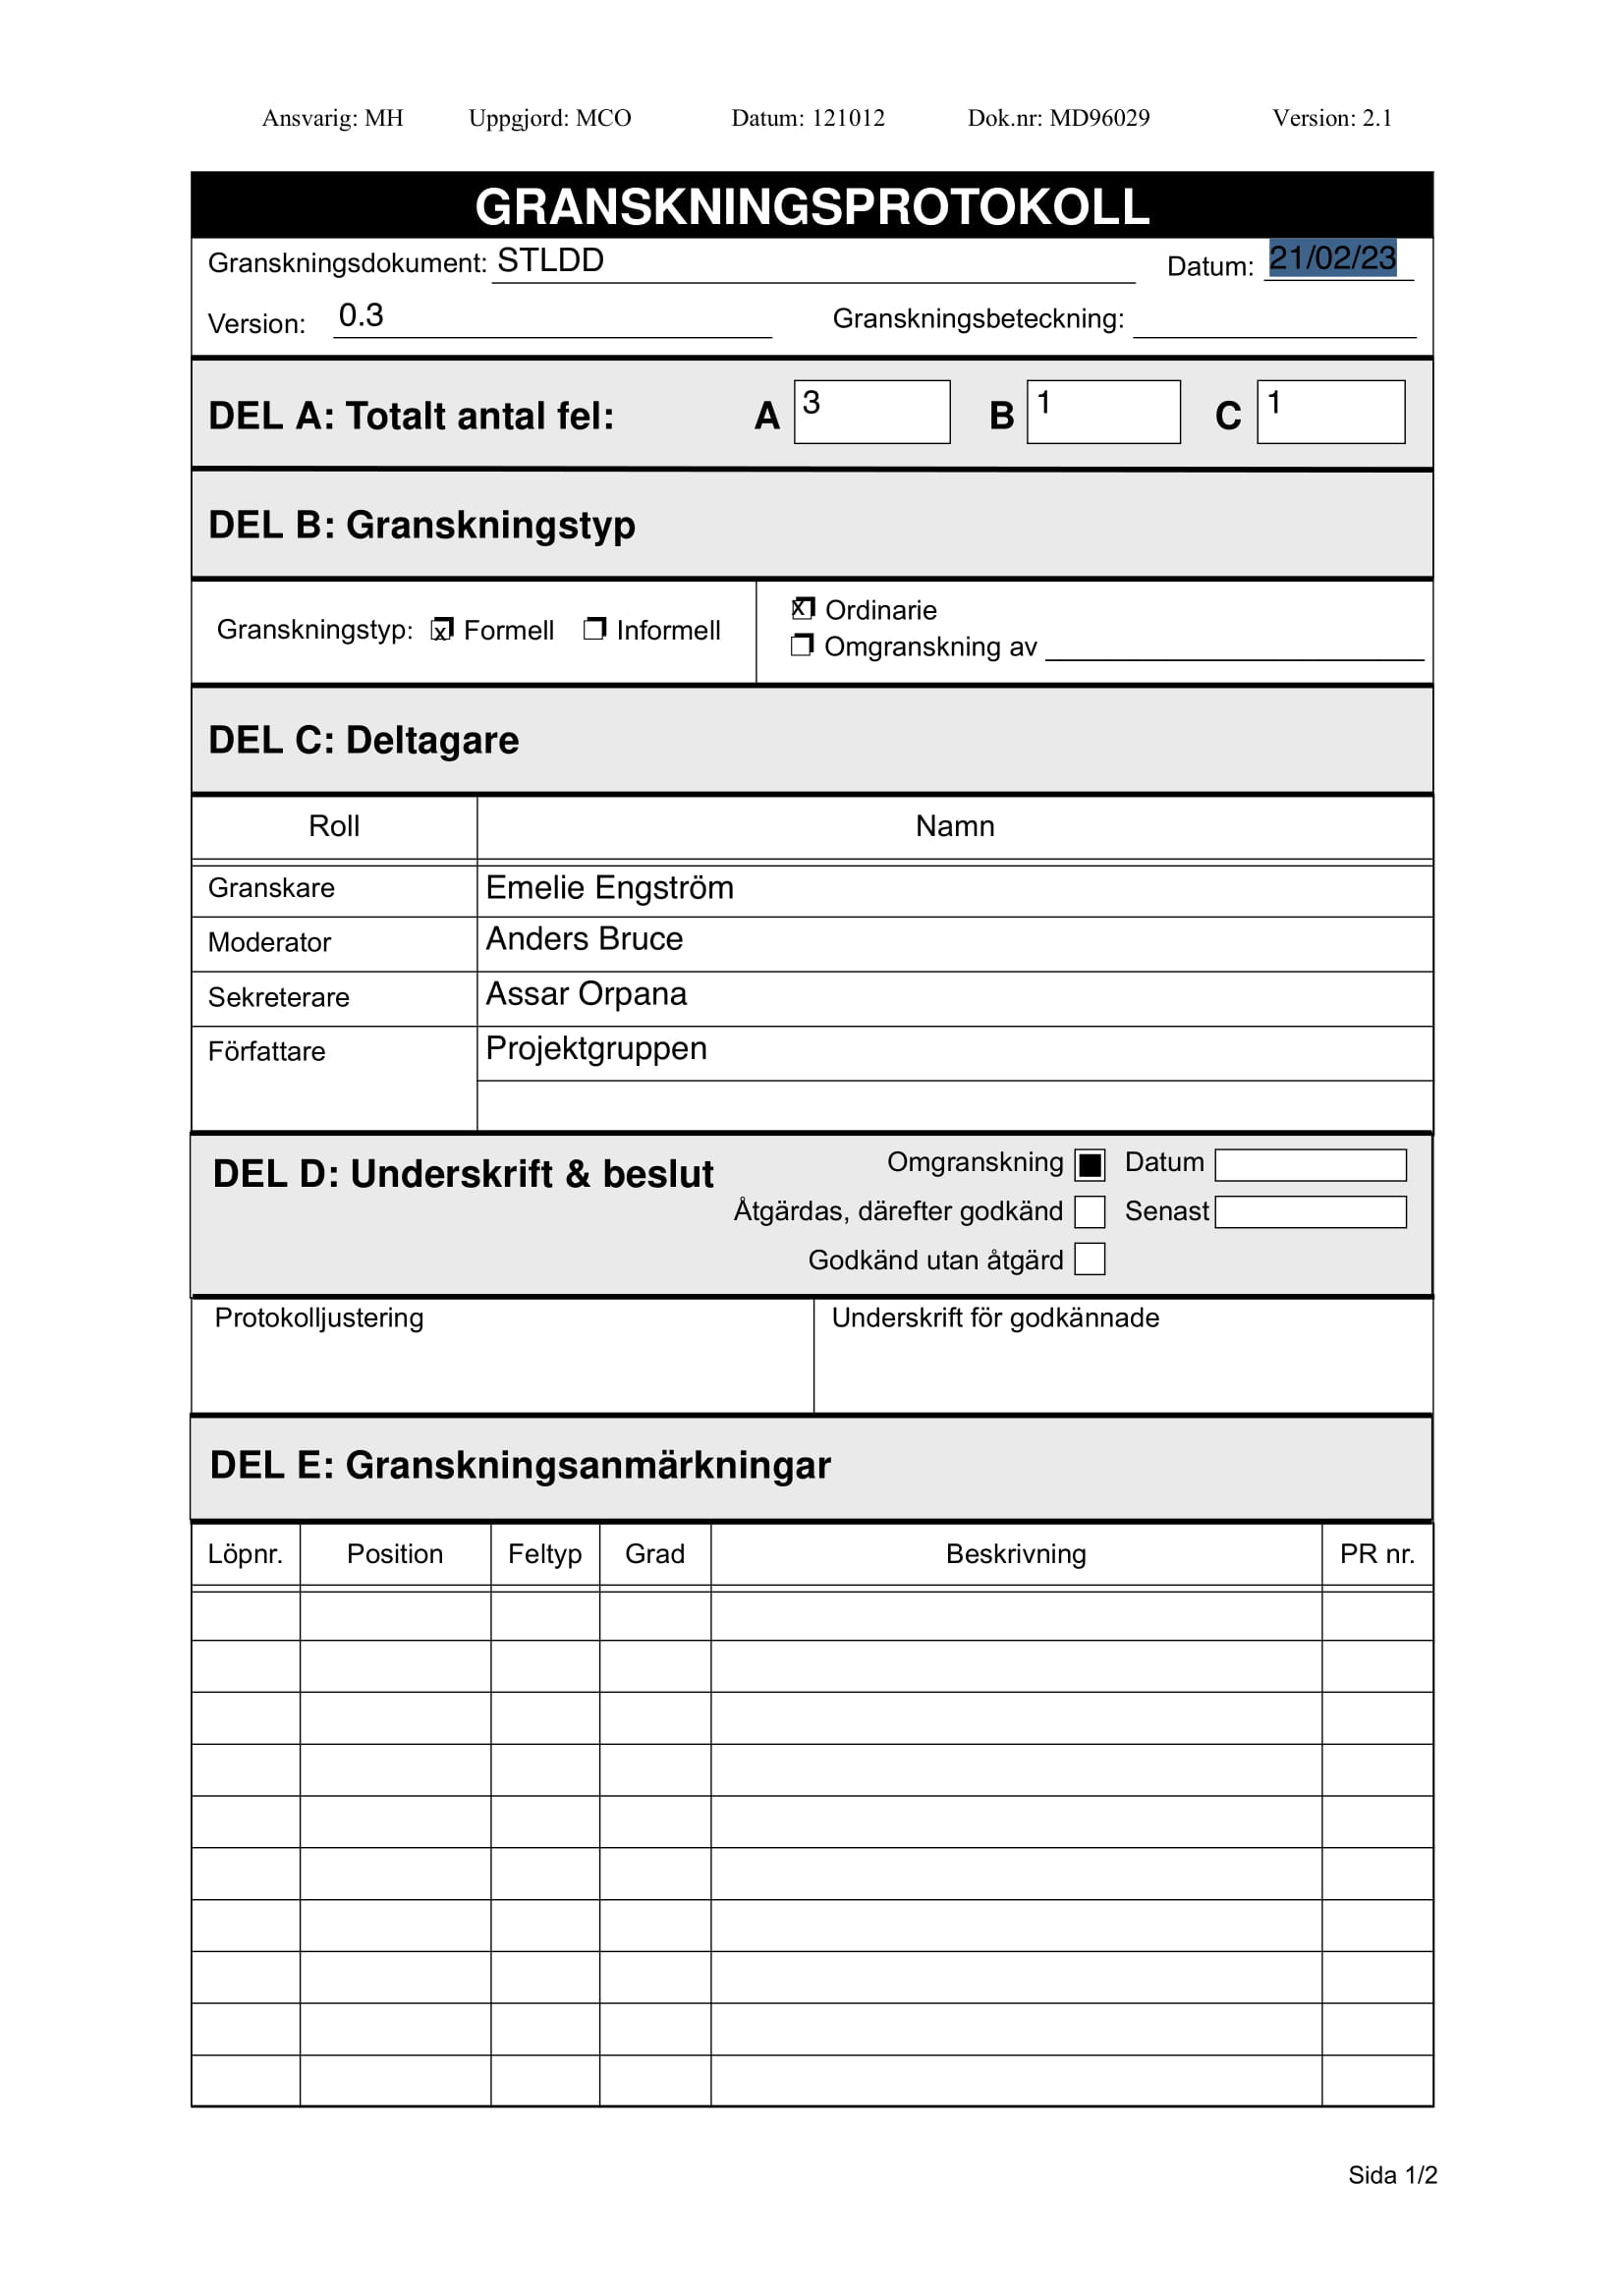
\includegraphics[width=13cm]{images/STLDD - Granskningsprotokoll-1}
     \renewcommand\figurename{Figure}
     \caption{Review Protocol for STLDD}
     \label{fig:my_label}
 \end{figure}

 
  \begin{figure}
     \centering
     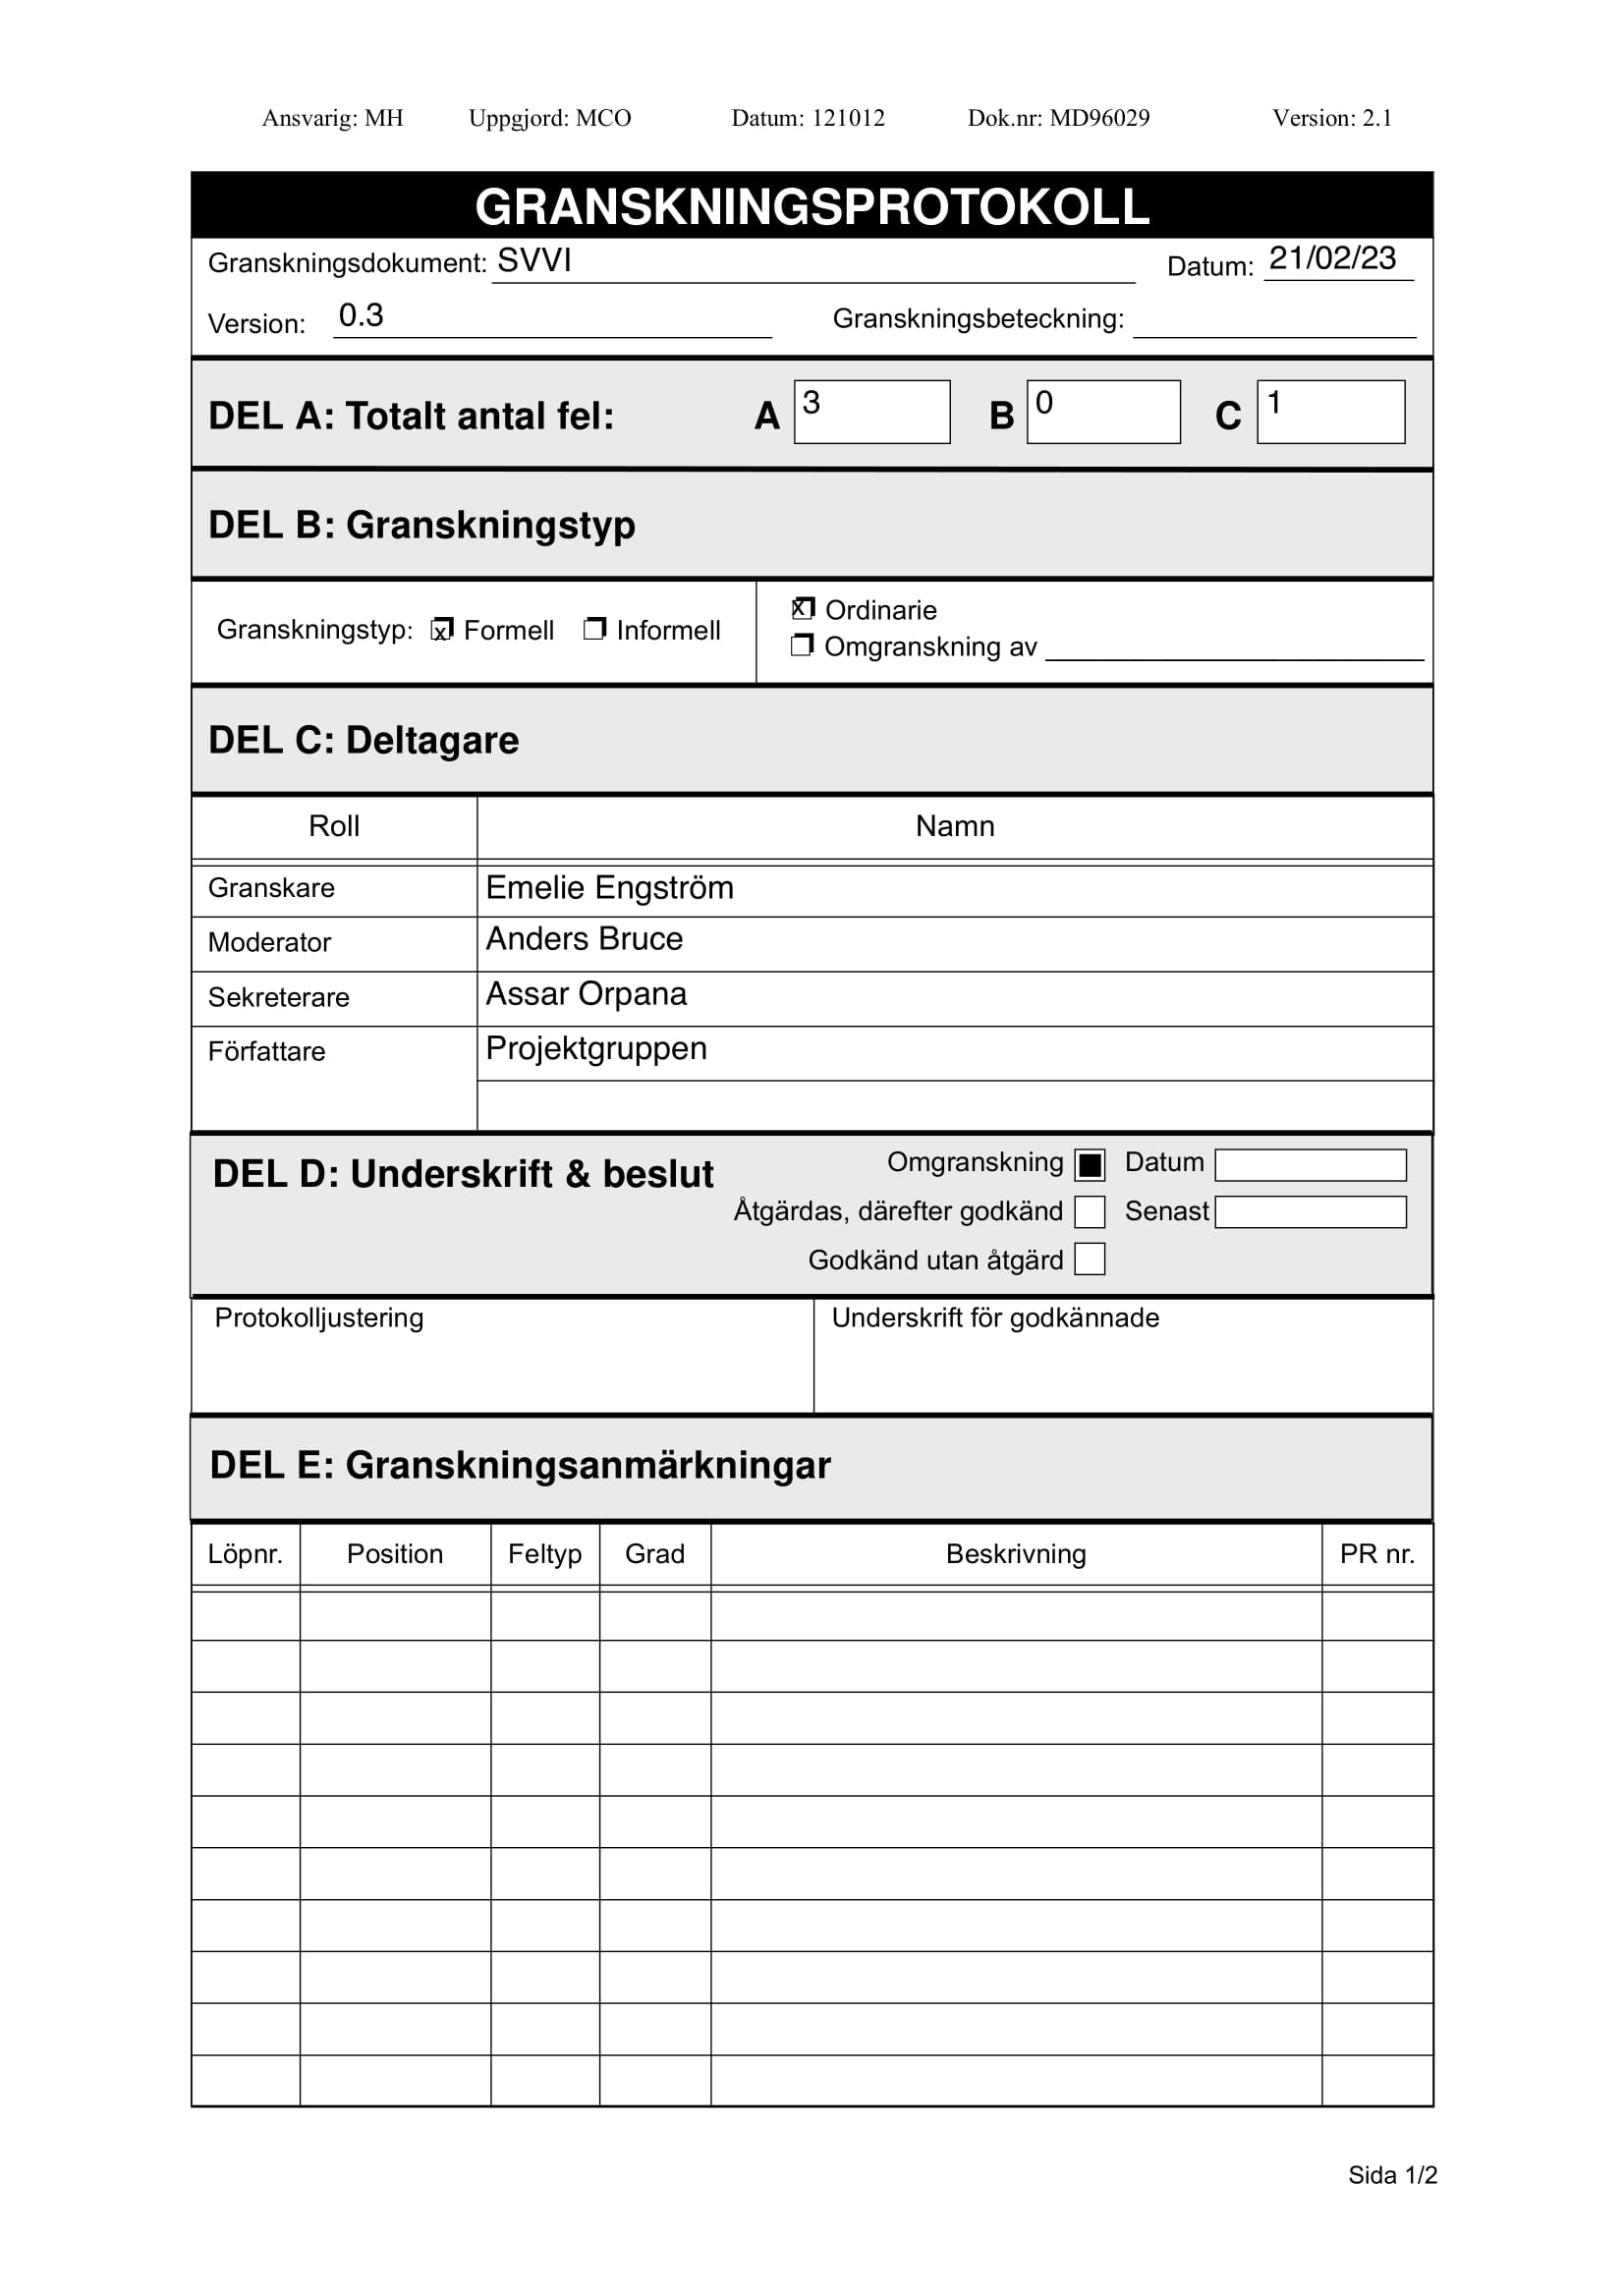
\includegraphics[width=13cm]{images/SVVI - Granskningsprotokoll-1}
     \renewcommand\figurename{Figure}
     \caption{Review Protocol for SVVI}
     \label{fig:my_label}
 \end{figure}
  
   \begin{figure}
     \centering
     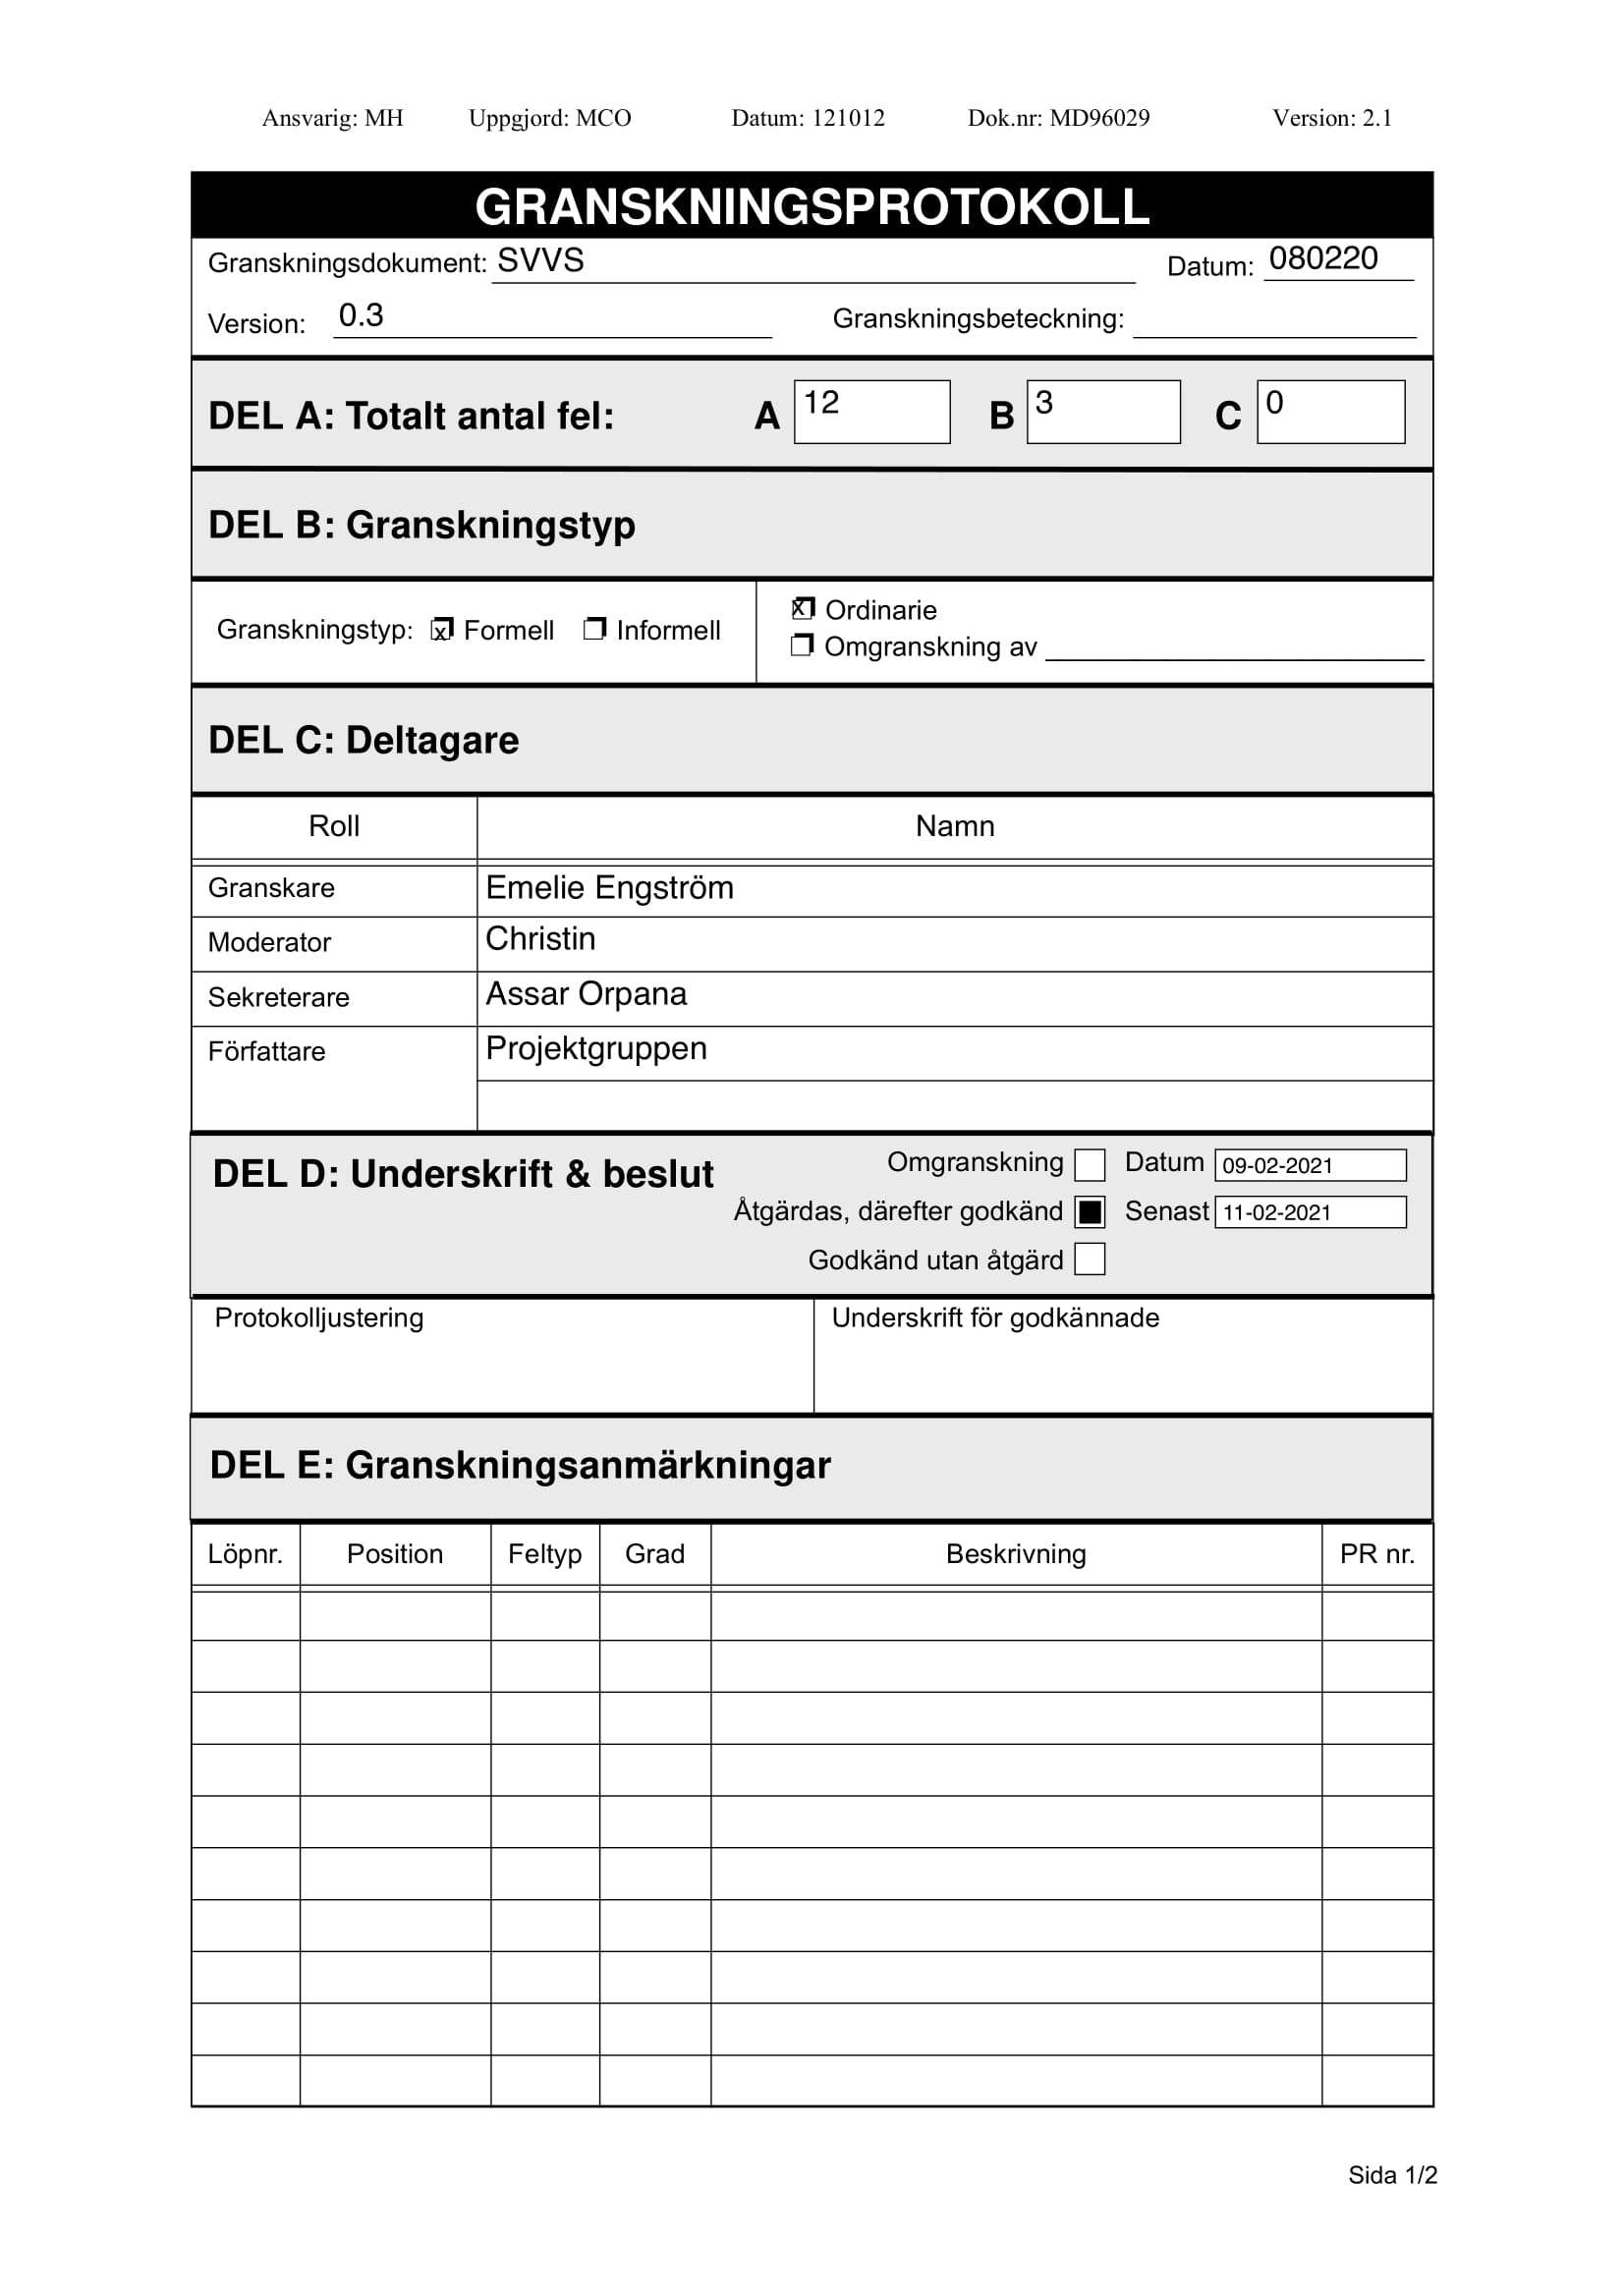
\includegraphics[width=13cm]{images/SVVS - Granskningsprotokoll-1}
     \renewcommand\figurename{Figure}
     \caption{Review Protocol for SVVS}
     \label{fig:my_label}
 \end{figure}
 
 
 \newpage
\begin{flushleft}
{\large \textbf{F. Informal Review Protocols}}
\end{flushleft}

\begin{figure}
     \centering
     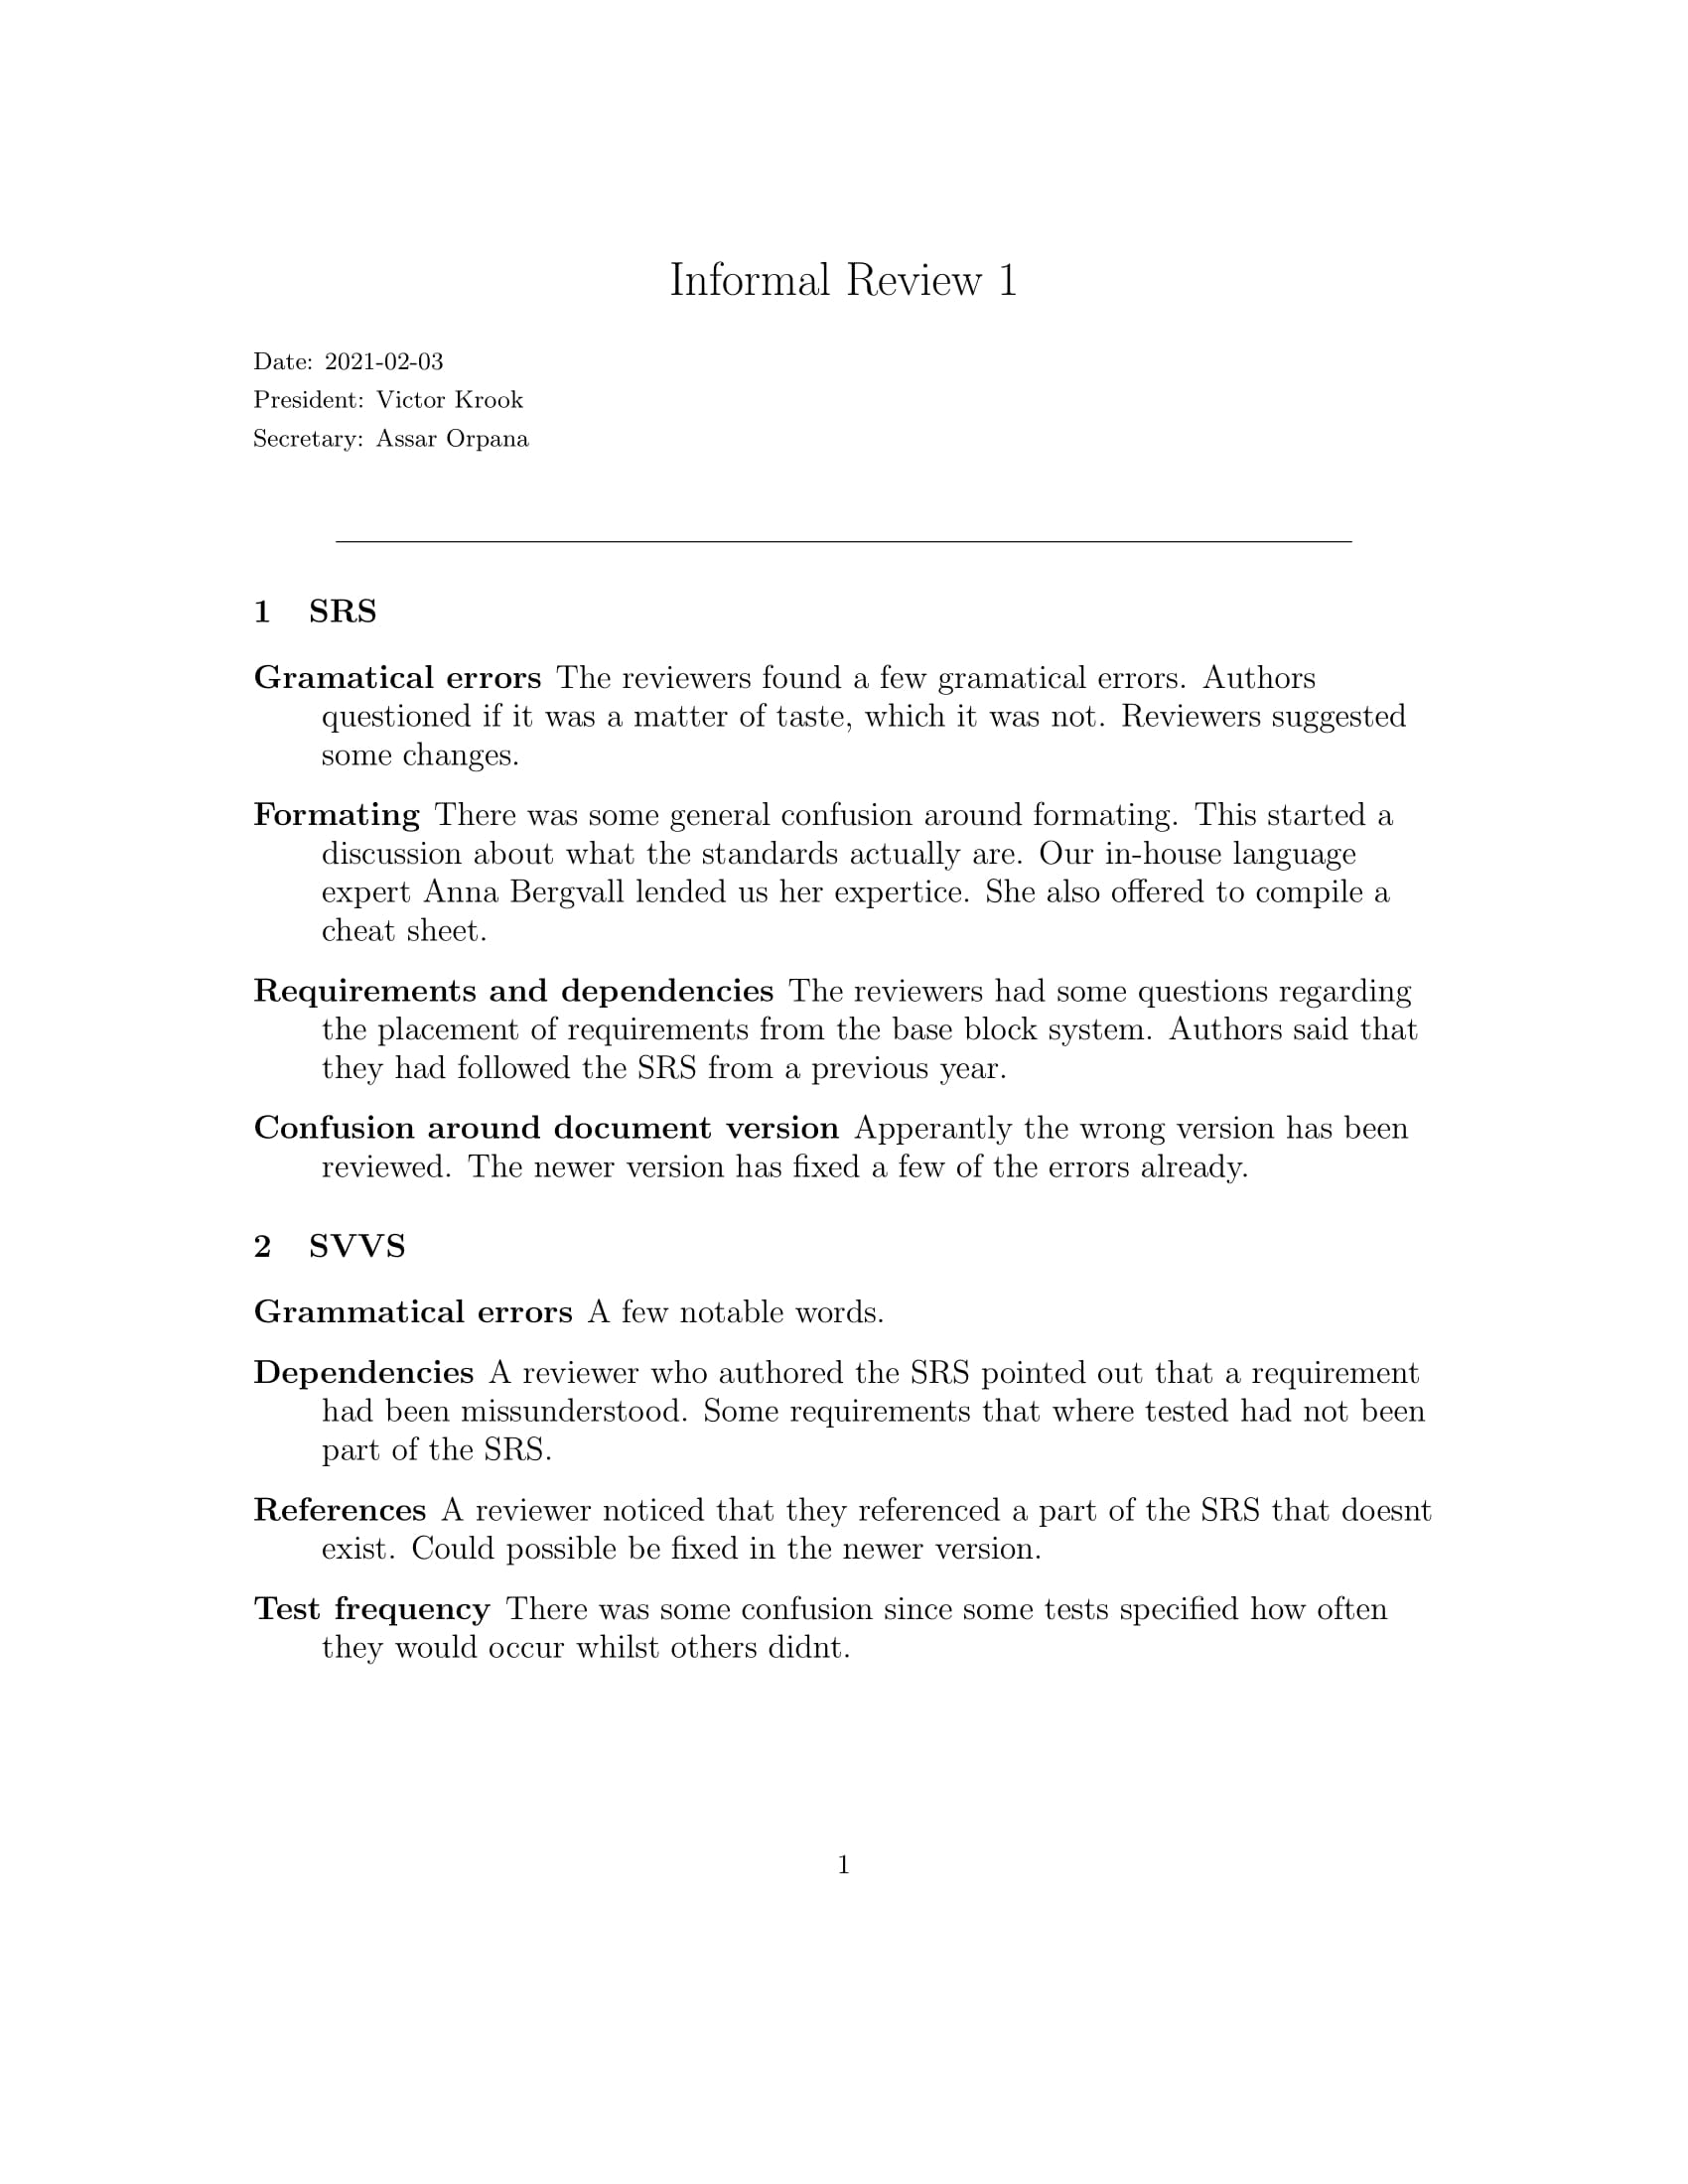
\includegraphics[width=13cm]{images/Phase1_2021_02_03-1}
     \renewcommand\figurename{Figure}
     \label{fig:my_label}
 \end{figure}
 
 
 \begin{figure}
     \centering
     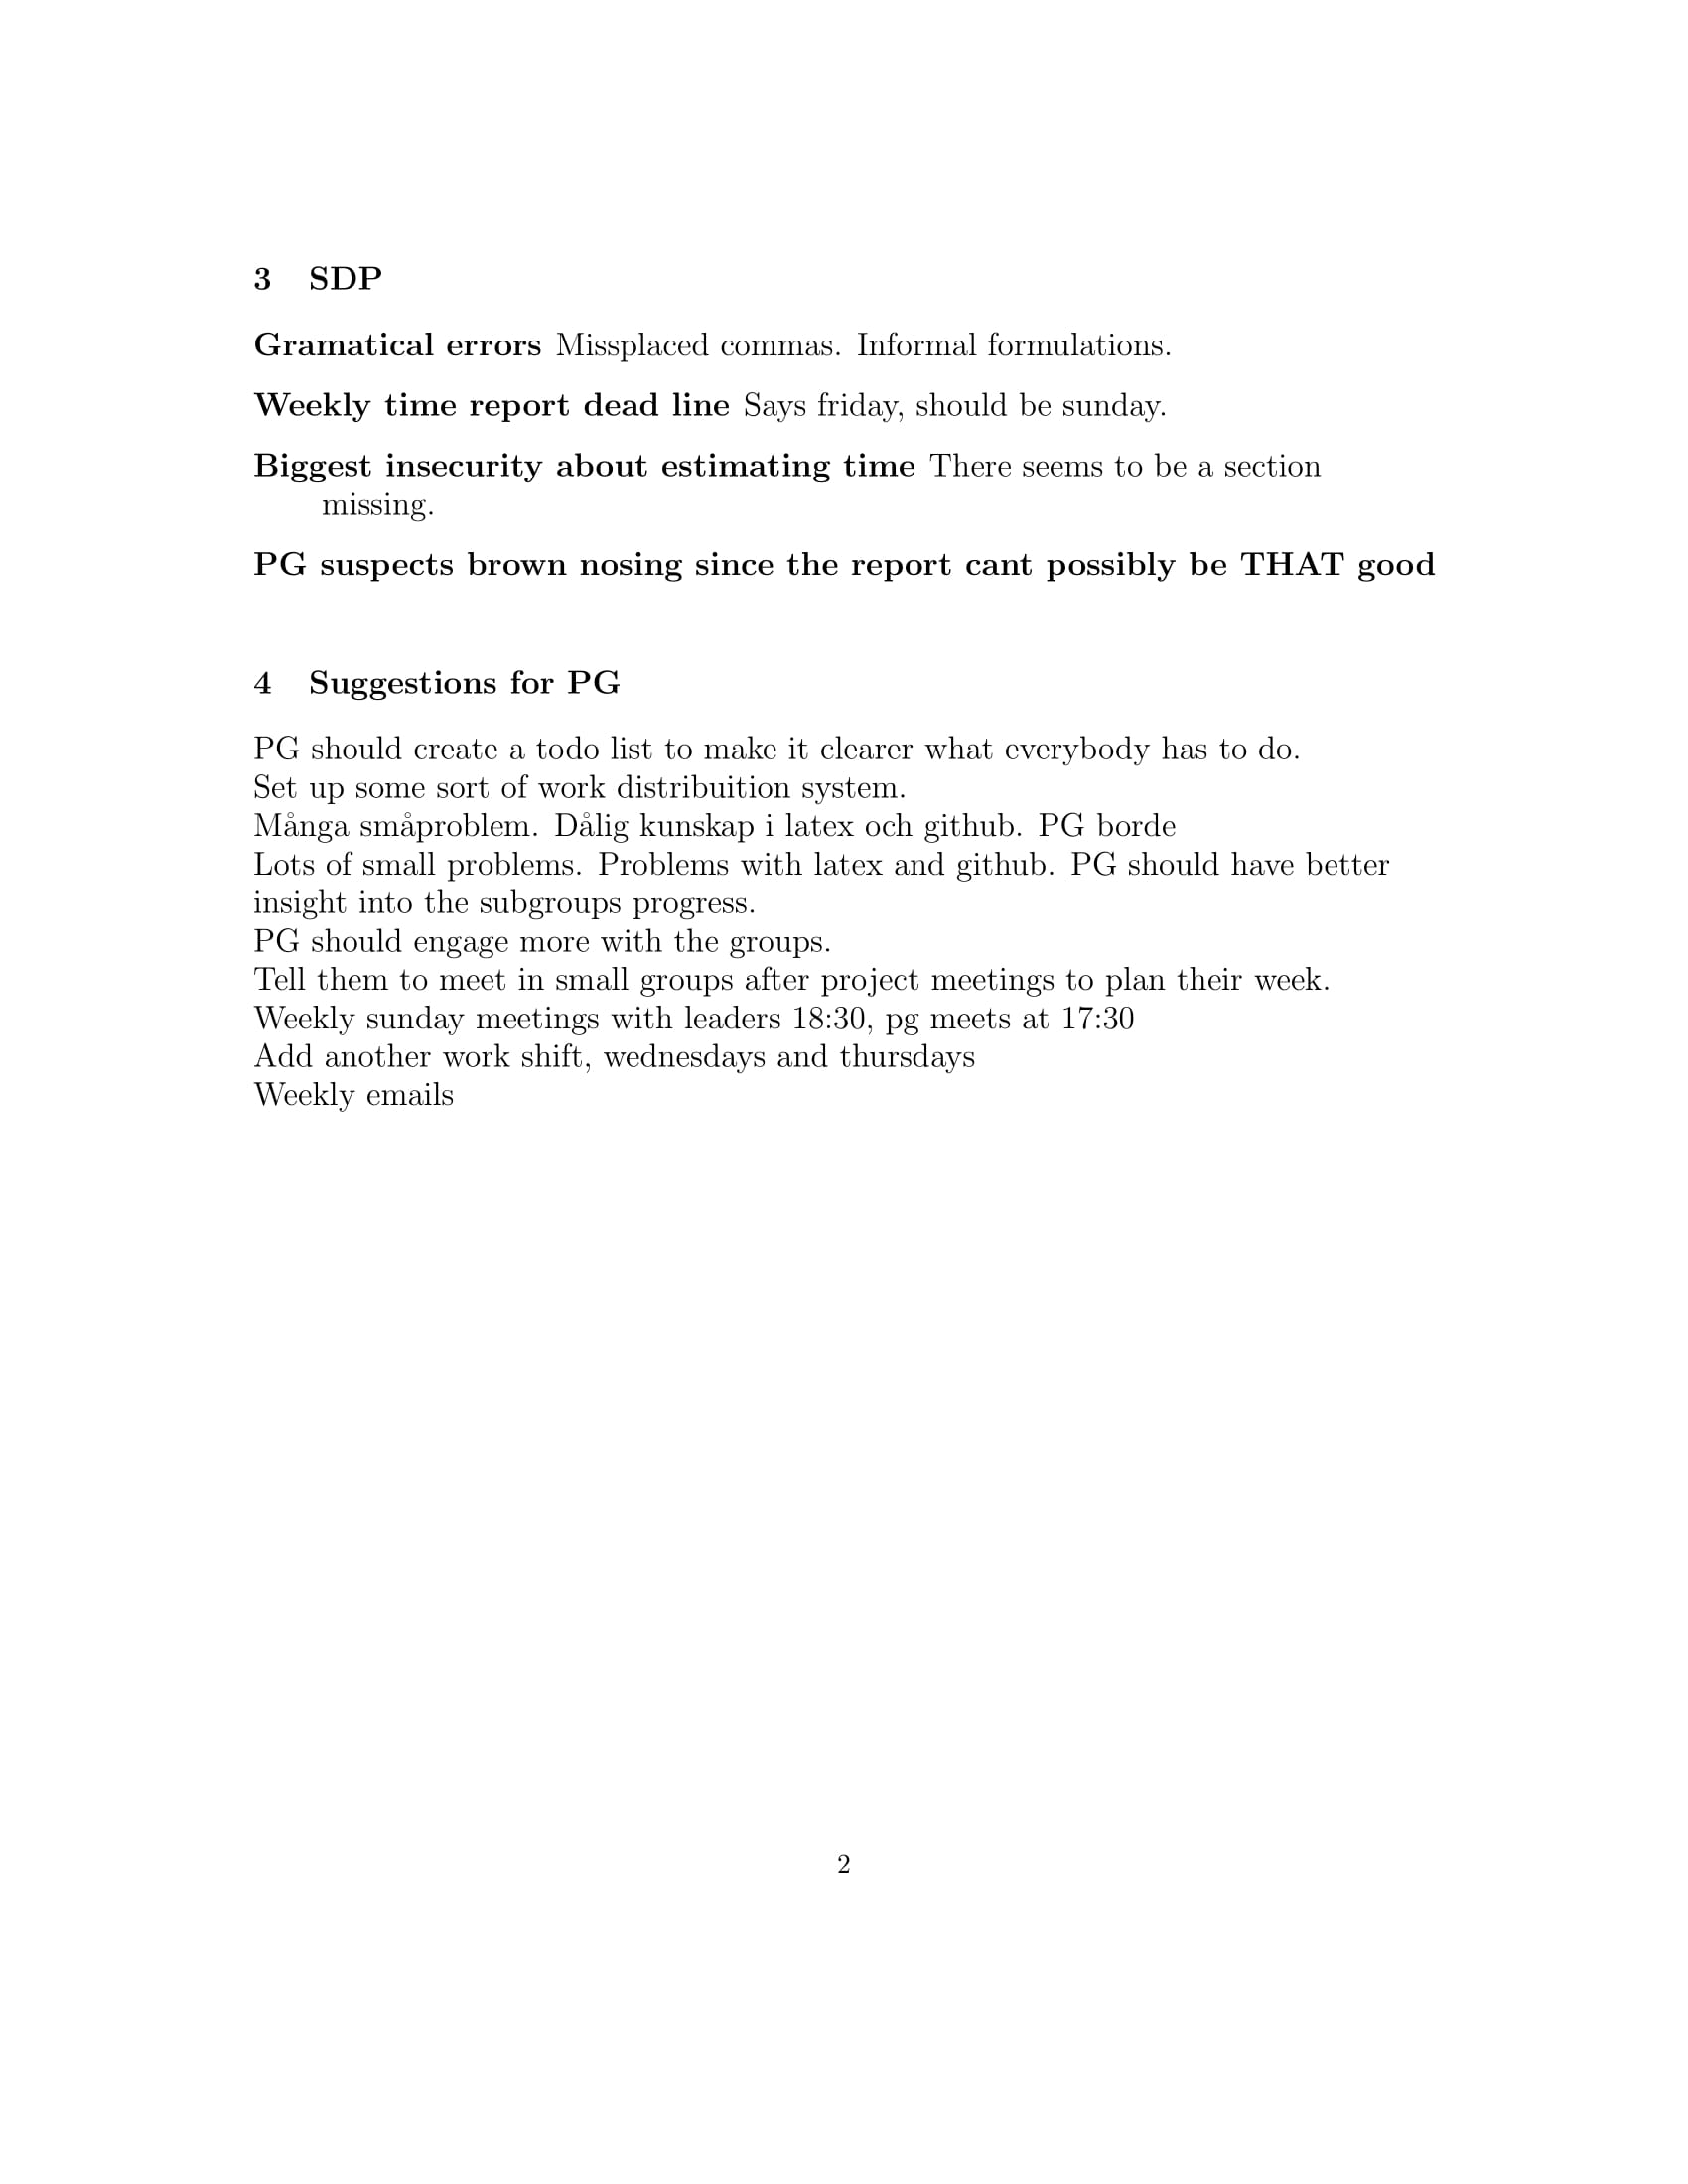
\includegraphics[width=13cm]{images/Phase1_2021_02_03-2}
     \renewcommand\figurename{Figure}
      \caption{Informal Review Protocol for phase one (1/2)}
     \label{fig:my_label}
 \end{figure}

\begin{figure}
     \centering
     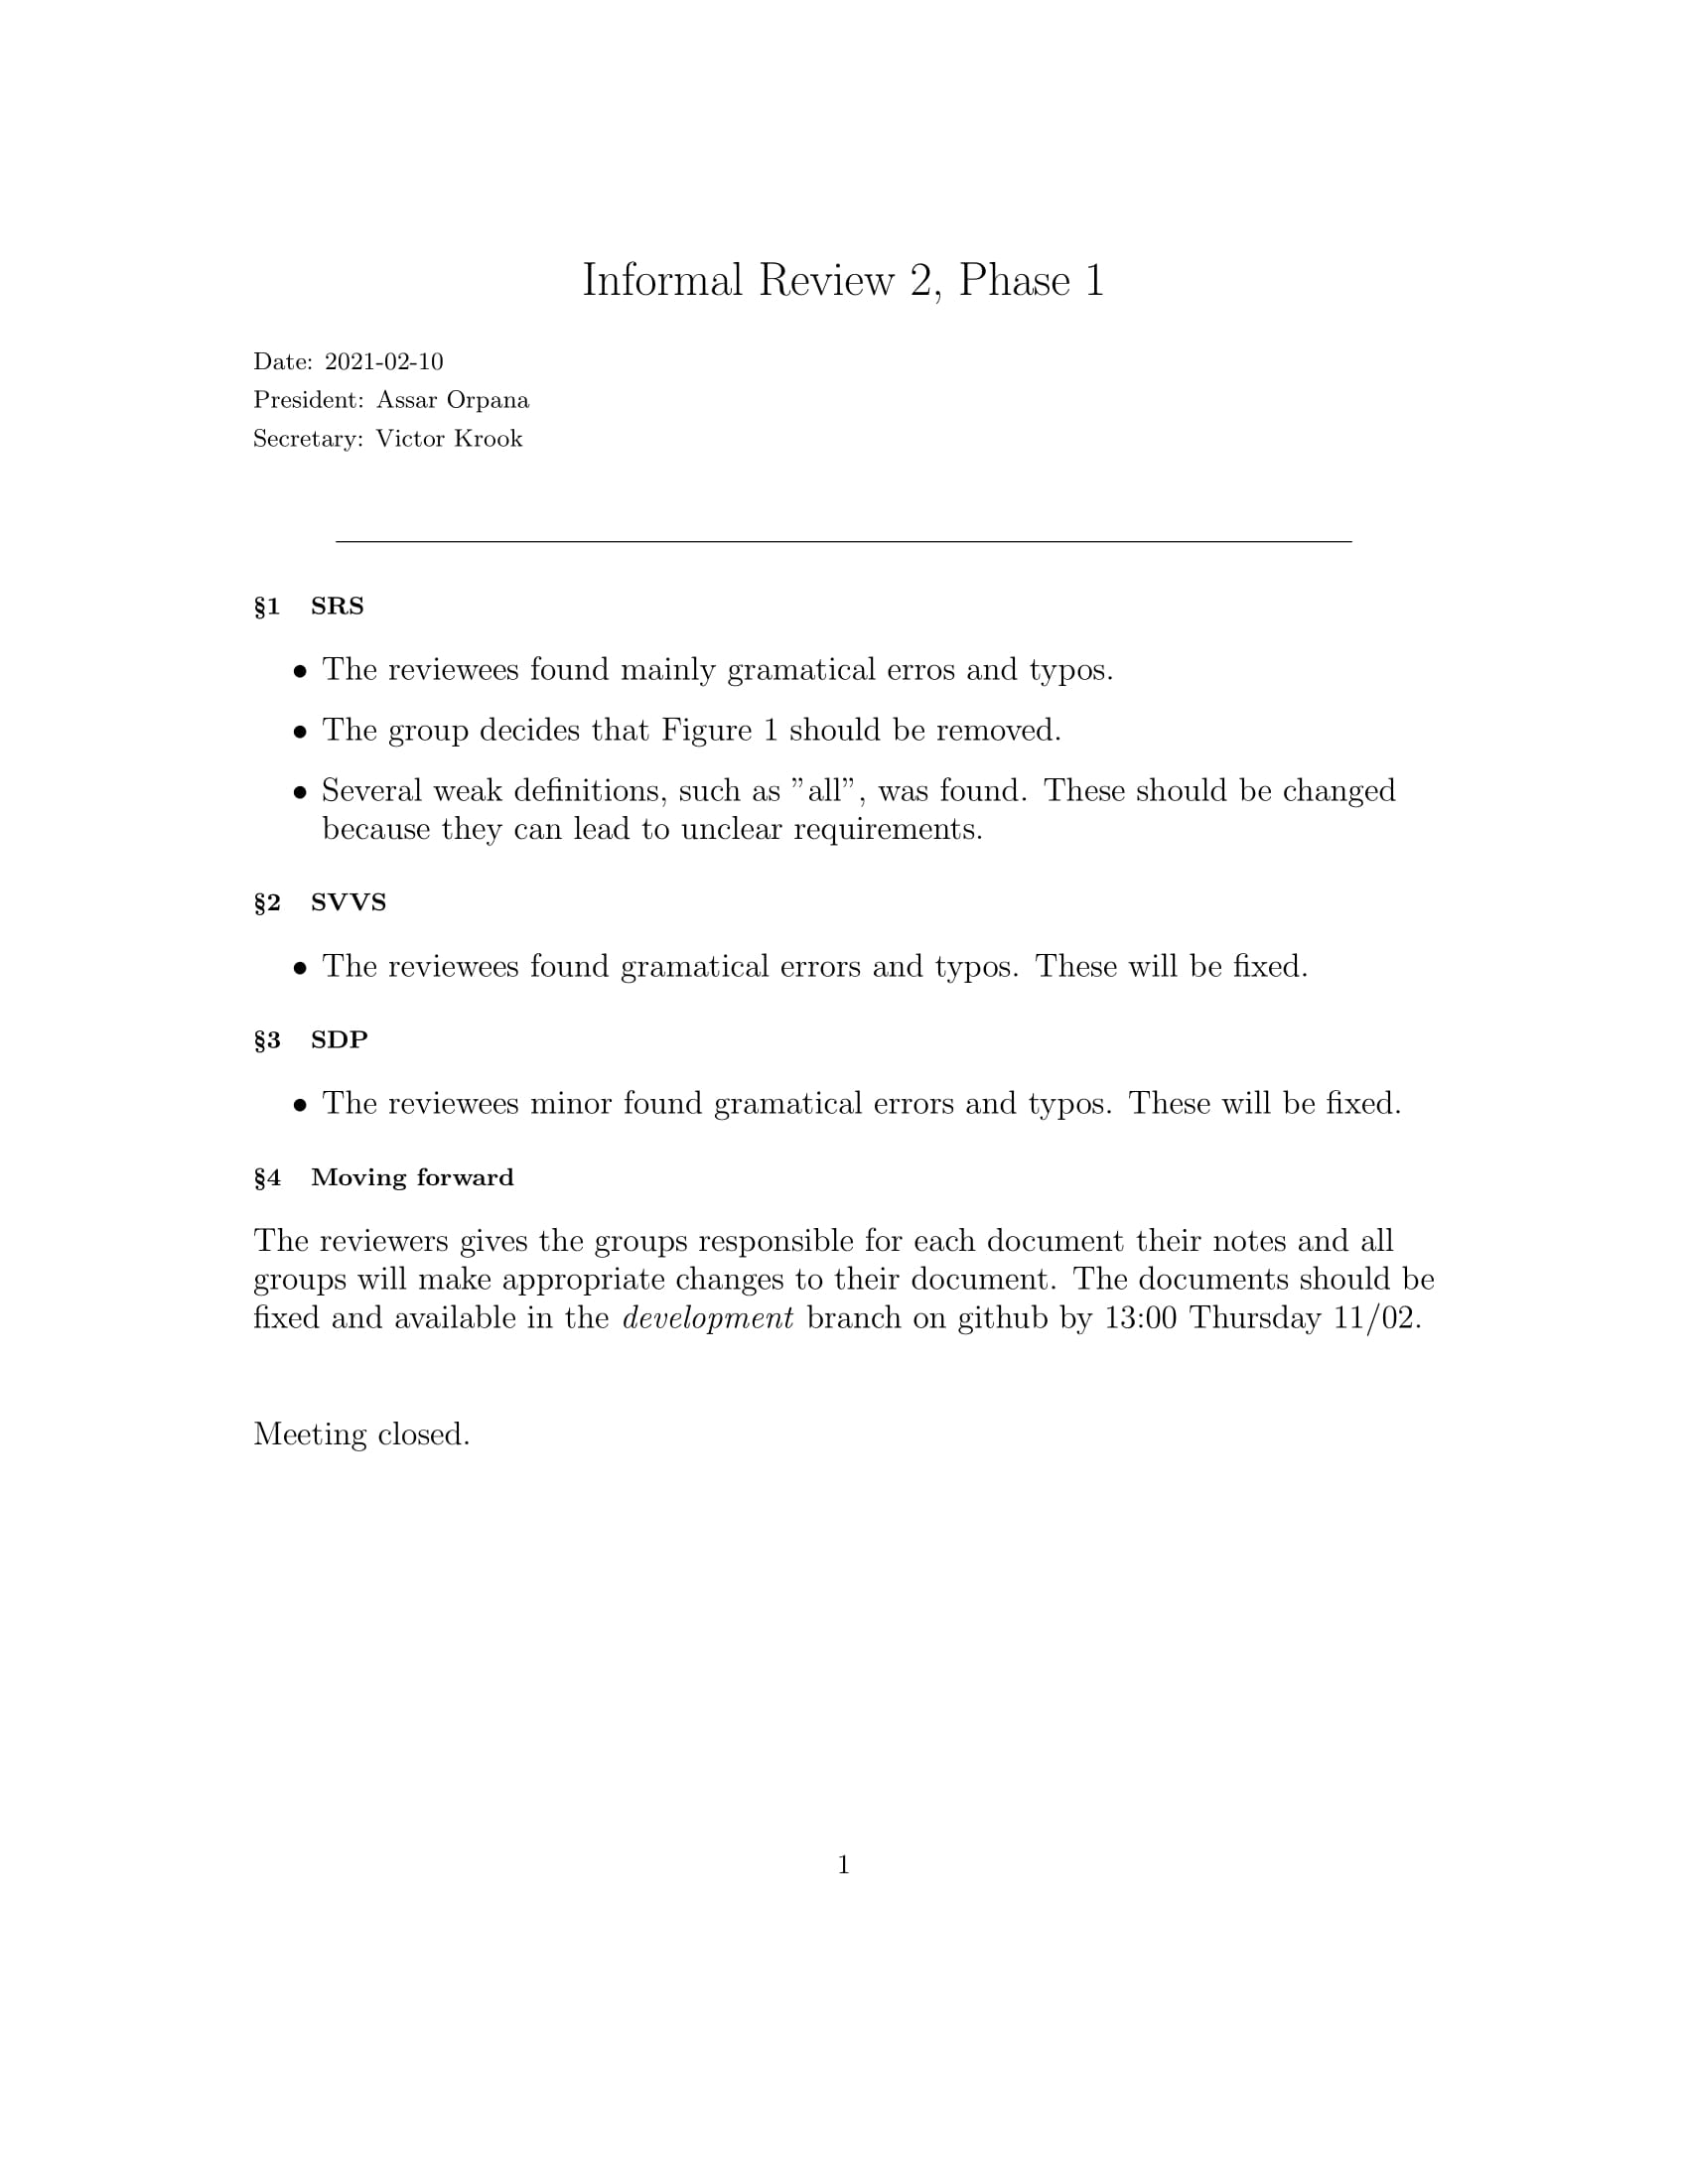
\includegraphics[width=13cm]{images/Phase1_2021_02_10-1}
     \renewcommand\figurename{Figure}
      \caption{Informal Review Protocol for phase one (2/2)}
     \label{fig:my_label}
 \end{figure}
 
 
 \begin{figure}
     \centering
     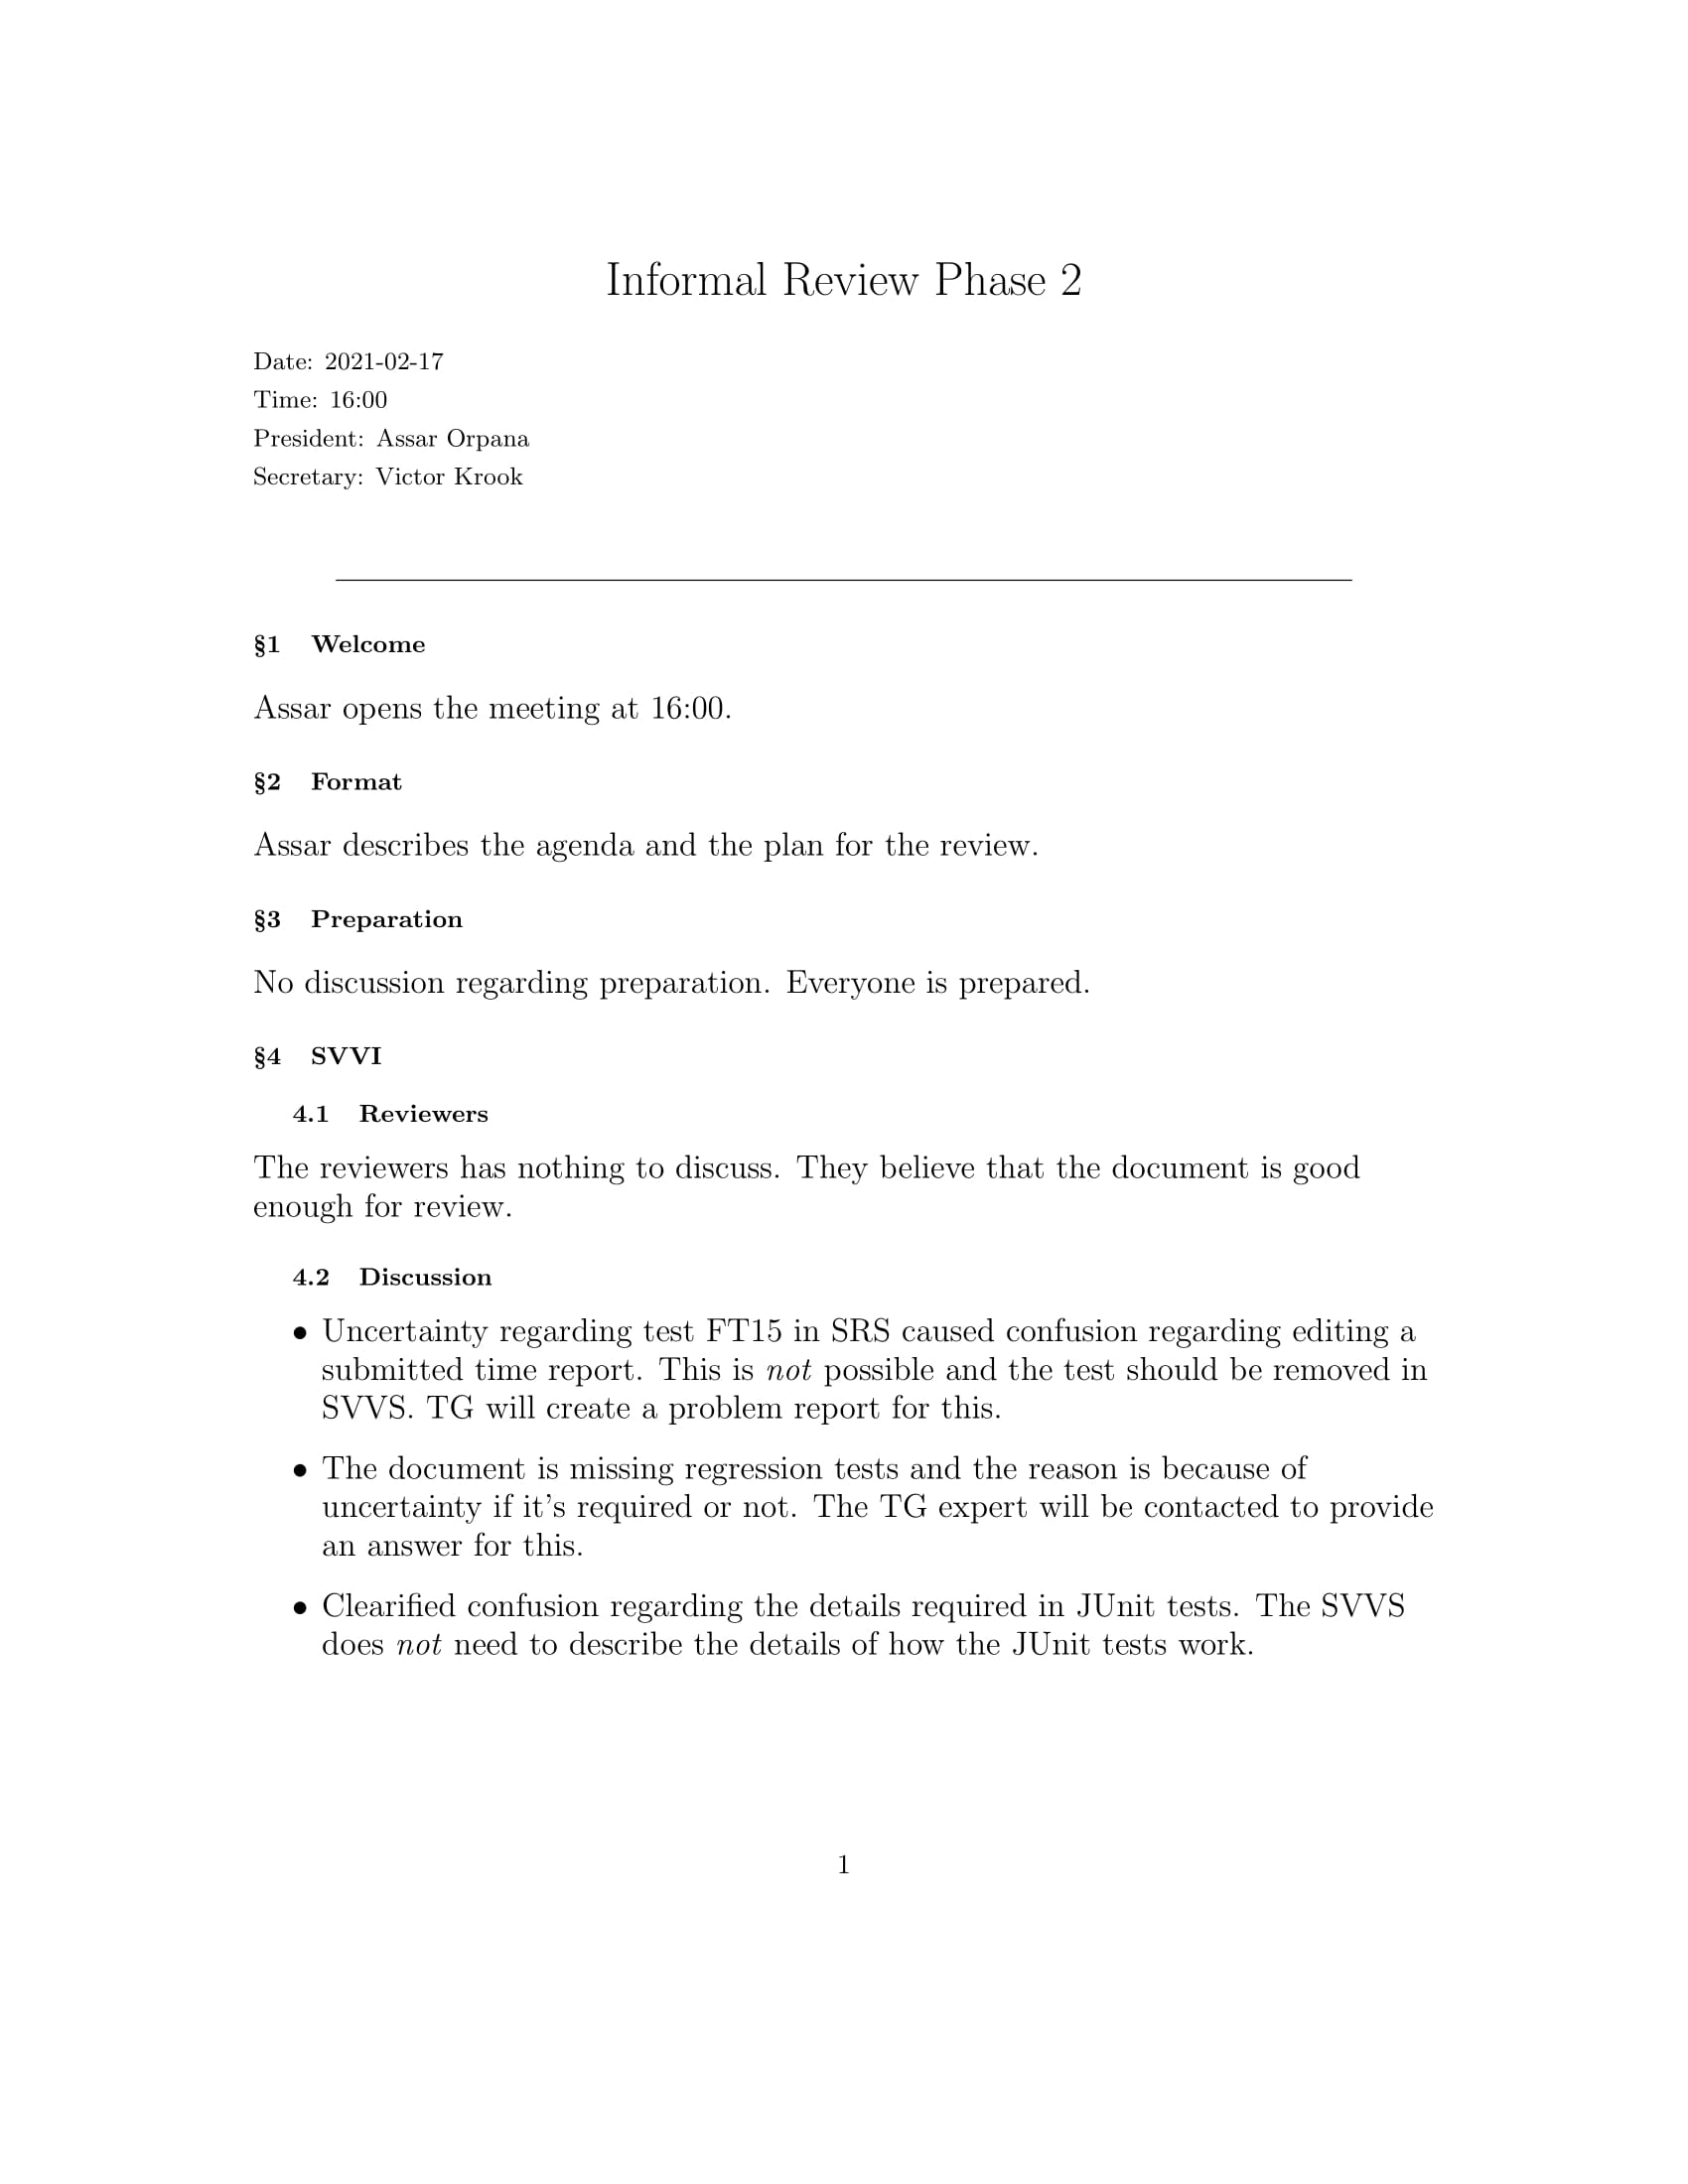
\includegraphics[width=13cm]{images/Phase2_2021_02_17-1}
     \renewcommand\figurename{Figure}
     \label{fig:my_label}
 \end{figure}
 
 
 \begin{figure}
     \centering
     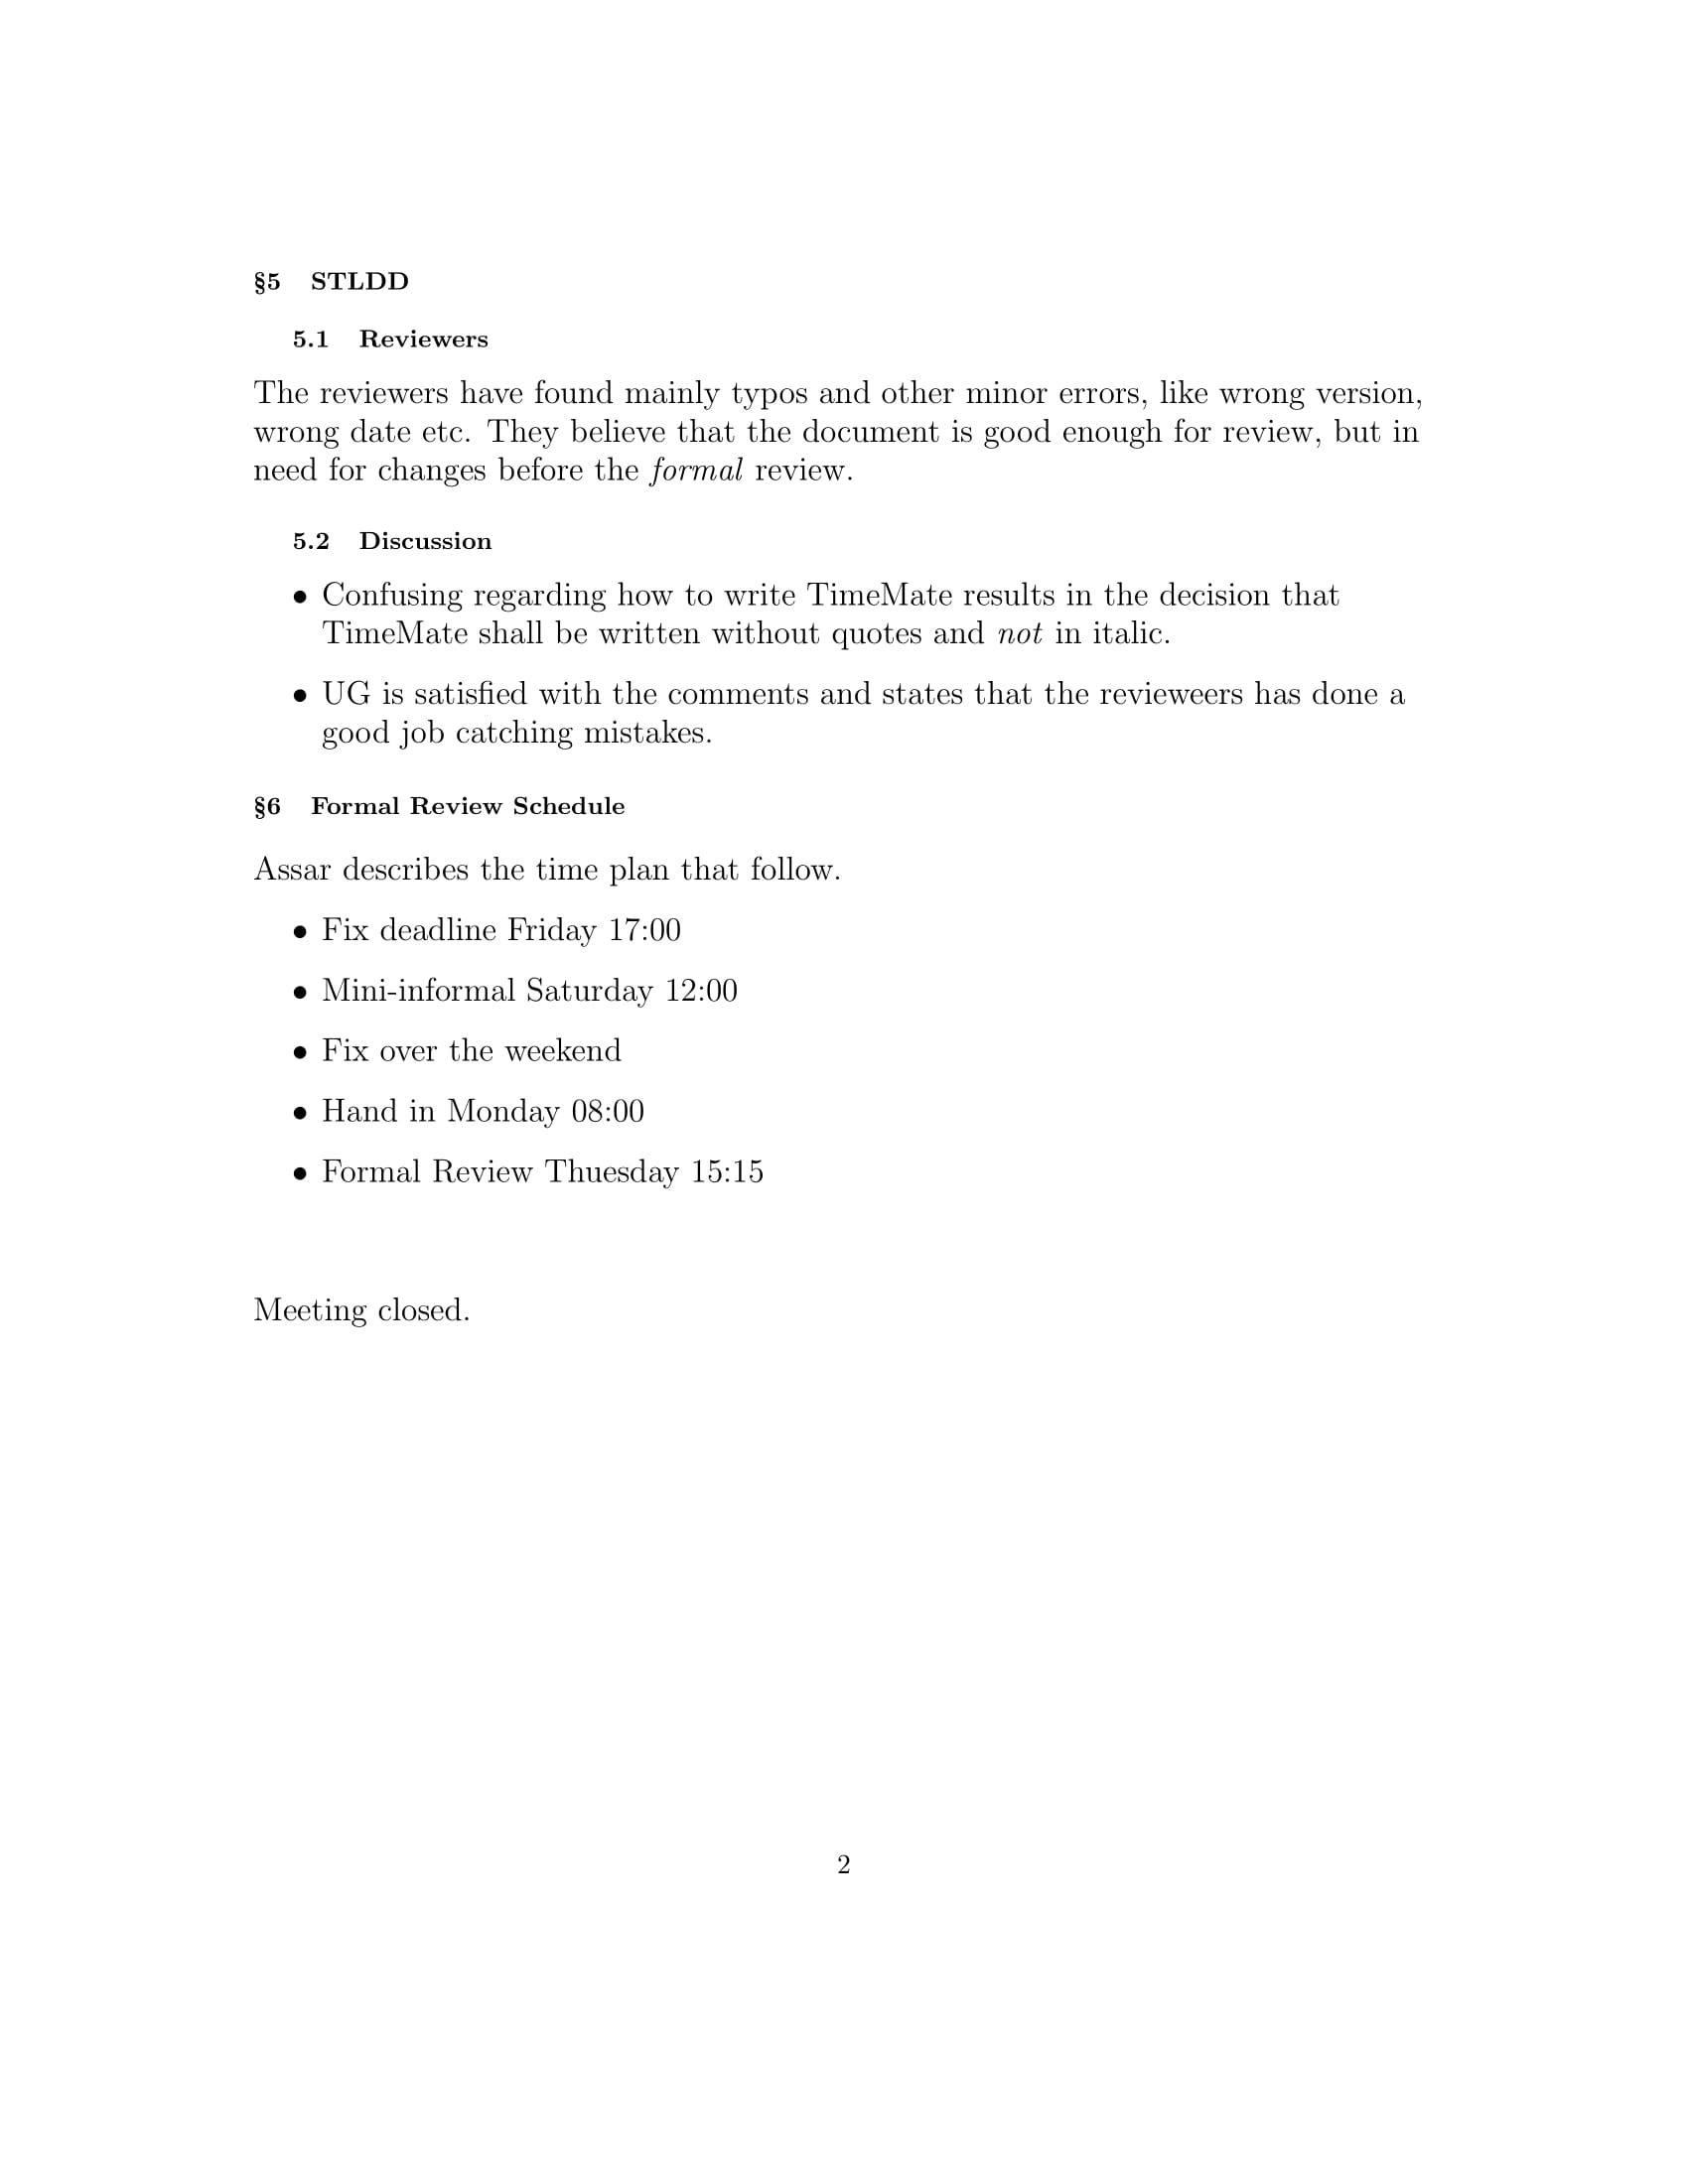
\includegraphics[width=13cm]{images/Phase2_2021_02_17-2}
     \renewcommand\figurename{Figure}
      \caption{Informal Review Protocol for phase two}
     \label{fig:my_label}
 \end{figure}
 
 
  \begin{figure}
     \centering
     \includegraphics[width=13cm]{images/Phase3_1_2021_03_05-1}
     \renewcommand\figurename{Figure}
      \caption{Informal Review Protocol for phase three (1/2)}
     \label{fig:my_label}
 \end{figure}
 
  \begin{figure}
     \centering
     \includegraphics[width=13cm]{images/Phase3_2_2021_03_08-1}
     \renewcommand\figurename{Figure}
      \caption{Informal Review Protocol for phase three (2/2)}
     \label{fig:my_label}
 \end{figure}


%---------Document ends here-----------

\end{document}
